% !Mode:: "TeX:UTF-8"
\documentclass[Paper]{skythesis}
%\renewcommand{\encodingdefault}{T1}
%\renewcommand{\familydefault}{cmbr}
\graphicspath{{preface/figures/}{paper/figures/}}  % 图路径
\begin{document}
%% 信息填写
%论文题目:{中文}
\skytitle{多品种装配车间调度研究}
%论文英文题目:
\Skytitle{A study of multi job in assembly shop}
%作者:{中文姓名}{学号}
\skyauthor{陈晟恺}{201002750102}
%拼音
\Skyauthor{CHEN Sheng-kai}
%指导教师:{导师中文名}
\skymentor{鲁建厦、董巧英}
%拼音
\Skymentor{LU Jian-sha, Dong Qiao-ying}
%个人信息:{毕业年份}{专业}
\skyinfo{2014}{工业工程}
%班级
\skyclass{健行1001}
%学院信息:{学院中文}
\skycollege{健行学院}
%英文信息
\Skycollege{Jianxing Honor College}
%学校名称:
\skyschool{浙江工业大学}
%英文校名
\Skyschool{Zhejiang University of Technology}     % 个人信息
%% !Mode:: "TeX:UTF-8"
% !TEX root = ..\Literature_Translation.tex
%% 封面
%% 信息填写
%论文题目:{中文}
\skytitle{多品种装配车间调度研究}
%论文英文题目:
\Skytitle{A study of multi job in assembly shop}
%作者:{中文姓名}{学号}
\skyauthor{陈晟恺}{201002750102}
%拼音
\Skyauthor{CHEN Sheng-kai}
%指导教师:{导师中文名}
\skymentor{鲁建厦、董巧英}
%拼音
\Skymentor{LU Jian-sha, Dong Qiao-ying}
%个人信息:{毕业年份}{专业}
\skyinfo{2014}{工业工程}
%班级
\skyclass{健行1001}
%学院信息:{学院中文}
\skycollege{健行学院}
%英文信息
\Skycollege{Jianxing Honor College}
%学校名称:
\skyschool{浙江工业大学}
%英文校名
\Skyschool{Zhejiang University of Technology}
\thispagestyle{empty}
\pdfbookmark[0]{封~~面}{thesiscover}
\phantomsection \label{thesiscover} %无形节命令
\newcommand\midtitle{}

\ifskythesis
  \renewcommand\midtitle{毕业论文(毕业设计说明书)}
\fi
\ifskylandt
  \renewcommand\midtitle{毕业论文(文献综述、外文翻译)}
\fi
\ifskyproposal
  \renewcommand\midtitle{毕业论文(开题报告)}
\fi
\vspace*{10mm}
% 校名
\begin{center}
   
\includegraphics[height=42pt,trim= 0 300 0 0]{zjutlogo}{\stxingkai\juhao{~浙江工业大学}}
\end{center}
\vspace*{12mm}
\centerline{\linespread{1.5}\yihao\bfseries\fangsong\midtitle}
\vspace*{19mm}

\renewcommand{\arraystretch}{1.0} %列表行距
\hspace*{3mm} 

{\sfzhongsong\zihao{1}{题目}
\hspace{0mm} 
\begin{minipage}[t]{120mm} % 这里建议自行微调
 \centering 
 \renewcommand{\ULthickness}{1.2pt}
 \renewcommand{\CJKunderlinecolor}{\color{black}}
   \linespread{1.1}\CJKunderline{\quad\skytitlec\quad}
\end{minipage}
}

\vspace*{15mm}
\begin{center}
    %\setlength{\arrayrulewidth}{0.5pt}
    
    {\sfzhongsong\zihao{3}
    \renewcommand{\ULthickness}{1.2pt}
    \renewcommand{\CJKunderlinecolor}{\color{black}}
    \newcommand{\kdist}{\hspace{4em}}
    
        \renewcommand{\arraystretch}{1.5}
        \begin{tabular}{lc}
            专\hspace{2em}业:& \CJKunderline{\kdist\extt{\skymajor}\kdist} \\ 
            班\hspace{2em}级: & \CJKunderline{\kdist\extt{\skyclassc}\kdist} \\
            学生姓名: &  \CJKunderline{\kdist\extt{\skyauthornamec}\kdist}\\
            指导老师: & \CJKunderline{\kdist\extt{\skymentorc}\kdist} \\
        \end{tabular}
    }
\vfill

{\sfzhongsong\zihao{4} 2013 -- 2014学年}
\end{center}

      % 封面
\frontmatter
%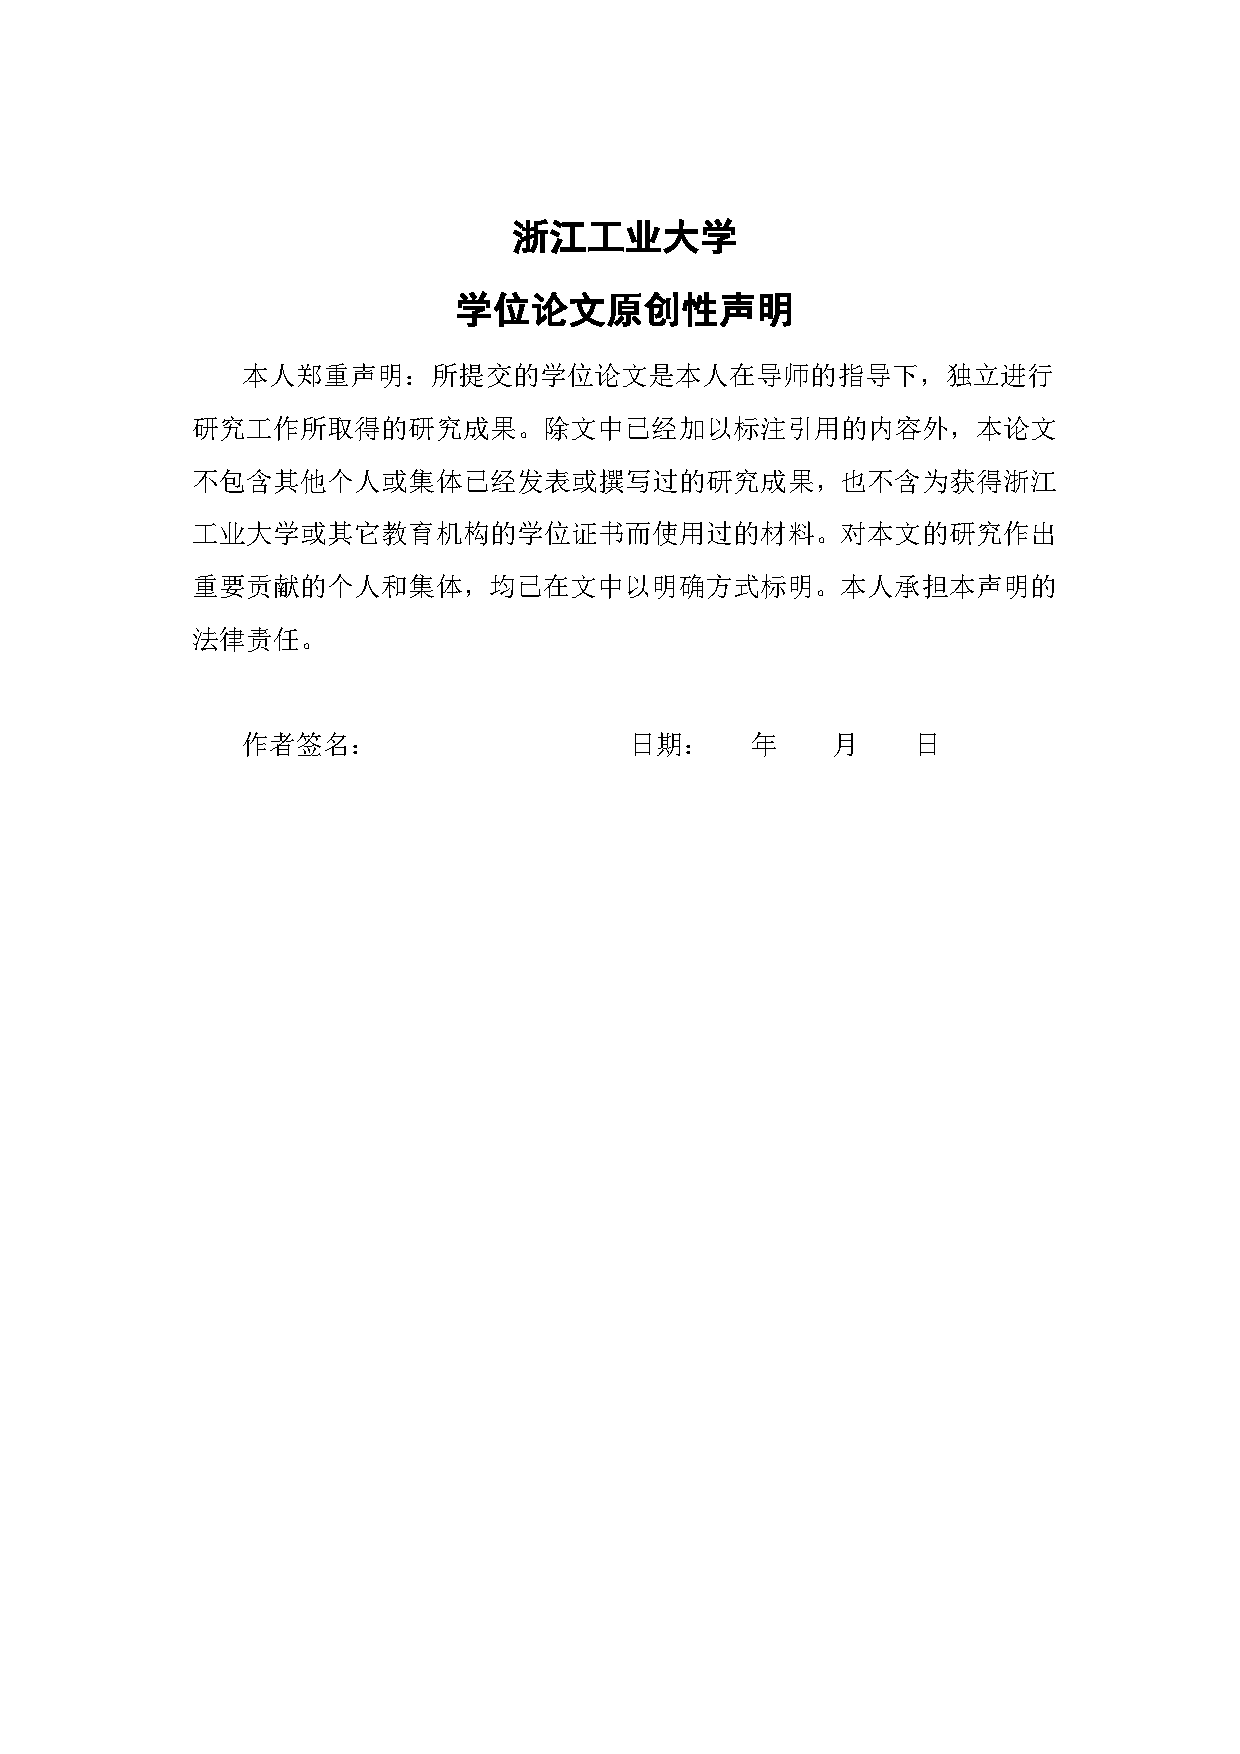
\includepdf{preface/statement}
\begingroup % 在组内的chapter不换行
\let\cleardoublepage\relax % chapter之后不换页
% !Mode:: "TeX:UTF-8"
% !TEX root = ..\paper.tex
\begin{abstractc}
\noindent \makebox[0pt][l]{\raisebox{8em}[0pt][0pt]{\songti\wuhao\bf 学号:\skyauthorid}}

\begin{center}
\vspace{-6mm}
{
\xiaosi

 学生姓名:\skyauthornamec\hspace{20mm} 指导老师:\skymentorc

\skyschoolc\skycollegec}
\end{center}
{\wuhao \songti \onequarterspacing
\noindent \textbf{摘要:}% !Mode:: "TeX:UTF-8"
本文针对某汽车电子零部件企业装配车间调度问题进行研究,该车间具有多条同质装配线,采用多品种、批量、面向主机厂的装配方式,存在提高产线利用率、降低冗余度、均衡生产等提升空间。突破主机厂限制是有效的解决方案,这是一个多品种多装配线轮番调度优化问题。

建立了$2$个调度优化模型,模型1 适用于订单到达稳定的情况,模型2 适用于不稳定的情况。两个模型都以加权拖延时间和与加权完成时刻和为主体,采用决策系数将之结合,模型2 需要考虑插单,引入和定义了产线闲置、流水线利用率、均衡率等概念以适应其情况,根据多品种和多流水线的特点,设计了相应的约束条件。在模型求解算法中,定义了虚拟序列的概念,将之与调度规则及启发式策略结合设计了交替改进(Cycle Amend, Cyc) 和虚拟序列(Virtual List, Vtr) 类多个求解算法。计算实验结果表明:Vtr -- Tabu 算法适用于中小规模的不考虑插单情况的问题,且随着工期目标的重视而凸显改进效果,VVT 算法的求解结果在多种不同决策环境下都显示出了较高的质量和稳定性。所提算法求解该模型是有效果的,所建模型也适合该问题。

本文所提的多品种多流水线轮番调度模型及其算法确实进一步提高了流水线利用率、按时交付等性能,仍存在如加入混流生产的改进空间。

\keywordsc{多品种多装配线,调度模型,虚拟序列,算法设计}
}
\end{abstractc}
\vspace{5mm}

\begin{abstracte}
\begin{center}
\vspace{1em}
{\xiaosi \onequarterspacing
 Author: \Skyauthorc\hspace{20mm} Mentor: \Skymentorc

\Skycollegec, \Skyschoolc

%{\xiaosan\bf\vbox{} Abstract}
}
\end{center}
{ 
\wuhao \onequarterspacing
\noindent \textbf{Abstract: } % !Mode:: "TeX:UTF-8"
Multi-type massive production usually takes part in the assembly line of electronic parts for auto-mobile, however, a myopic way that specialize assembly line by the main factories is widely used, so that low utilization , high redundancy and unbalance production always happens. A sound solution is to despecialize the assembly line, the implementation of this solution is a so called multi-type multi-assembly-line take-turn scheduling problem. In this study, 2 mathematical models is built for different levels of managenent to apply. With proposed concept of \textit{virtual list}, schedule rule and heuristic tactic, 5 algorithms: Cyc --ATC, Cyc -- ATCS, Cyc -- Tabu, Vtr -- Tabu, VVT in 2 classes are designed. Experiment takes with script in Python shows, that Vtr -- Tabu algorithm suits for small and median scale problem, especially for none-job-inseting high weighted date-related problem, while high stability and quality schedule in various aspects can be obtain with VVT algorithm.

\keywordse{~multi-type, multi-assembly-line, scheduling model, virtual list, algroithm design}}
\end{abstracte}
%\listoffigures             % 图目录
%\pagenumbering{Roman}
%\listoftables              % 表目录
%\pagenumbering{Roman}


%%%%%%%%%% 正文 %%%%%%%%%%
\mainmatter
\makeatletter
%\include{body/intros}

% !Mode:: "TeX:UTF-8"
\chapter{公式}
\section{公式}
\[\sideset{^\beta_a}{^\ast_\triangle}
\prod^{n}_{k=1},
\sideset{}{'}\sum_{m=1}^\infty E_{2m+1}\]

\begin{equation}
\label{equaa2}
\iiint_1^1\frac{f(x)}{\sqrt{1-x^2}}dx = \frac{\pi}{n}\sum_{k=1}^nf(cos\frac{2k-4}{2n})+\frac{\pi}{2^{2n-1}(2n)!}f^{(2n)}(\theta)+max+\max
\end{equation}



张图片独自占一行的插入形式如图\eqref{equaa2}~所示。
\chapter{456}
\section[see]{建立良}
造等新的IE技术、理念的出现,掀起各国企业学习和运用的热潮。作为IE技术的基础运用,工作研究是最基本的技术,也是其他新兴IE技术运用的基础。企业在学习各种新的IE技术和理念的之前,必须建立良好的基础,通过工作研究\footnote{来建立科学的生产作业流程和}时间标准,并对生产线进行持续地平衡优化。
%\begin{figure}[H]
%\centering
%\vspace{\baselineskip}
%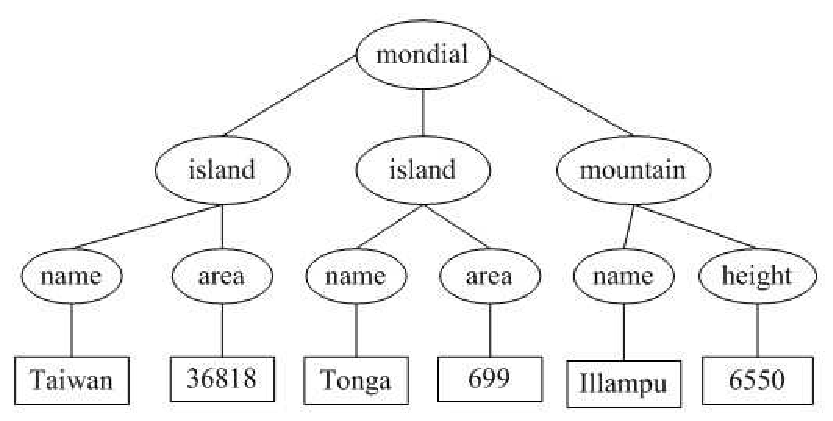
\includegraphics[width=0.4\textwidth]{XML}
%\caption{树状结构}\label{fig:xml}
%\vspace{\baselineskip}
%\end{figure}


掀起各国企业学习和运用的热潮。作为IE技术的基础运用,工作研究是最基本的技术,也是其他新兴IE技术运用的基础。企业在学习各种新的IE技术和\cite{2007}理念的之前,必须建立良好的基础,通过工作研究

\begin{table}[h]
  \centering
  \vspace{\baselineskip}
\caption{我问}
    \begin{tabular}{lcccccc}
    \toprule
    Source & Sourcer1 & Sourcer2 & Sourcer3 & Sourcer4 & Sourcer5 & Sourcer6 \\
    \midrule
    ModelEntity.EntityTpe & 7     & 8     & 9     & 10    & 11    & 12 \\
    \bottomrule
    \end{tabular}%
\end{table}%

掀起各国企业学习和运用的热潮。作为IE技术的基础运用,工作研究是最基本的技术,也是其他新兴IE技术运用的基础。企业在学习各种新的IE技术和理念的之前,必须建立良好的基础,通过工作研究\cite{McDonnell1994}
\section{IE技术}
\subsection{建立良}
掀起各国企业学习和运用的热潮。作为IE技术的基础运用,工作研究是最基本的技术,也是其他新兴IE技术运用的基础。企业在学习各种新的IE技术和理念的之前,必须建立良好的基础,通过工作研究
\subsection{IE技术}
\subsubsection{的基础}
的热潮。作为IE技术的基础运用,工作研究是最基本的技术,也是其他新兴IE技术运用的基础。企业在学习各种新的IE技术和理念的之前,必须建立良好的基础,通过工作研究
\subsubsection{的基础}
的热潮。作为IE技术的基础运用,工作研究是最基本的技术,也是其他新兴IE技术运用的基础。企业在学习各种新的IE技术和理念的之前,必须建立良好的基础,通过工作研究
\section{建立良}
sfasf
fgdfg
\section{单张图片的插入方法}
单张图片独自占一行的插入形式如所示。


\chapter{公式}
\section{公式}
$\sideset{^\beta_a}{^\ast_\triangle}
\prod^{n}_{k=1},
\sideset{}{'}\sum_{m=1}^\infty E_{2m+1}$

\begin{equation}
\label{equaa}
\iiint_1^1\frac{f(x)}{\sqrt{1-x^2}}dx = \frac{\pi}{n}\sum_{k=1}^nf(cos\frac{2k-4}{2n})+\frac{\pi}{2^{2n-1}(2n)!}f^{(2n)}(\theta)+max+\max
\end{equation}

张图片独自占一行的插入形式如图\eqref{equaa}~所示。
%\include{body/tables}
%\include{body/equations}
%\include{body/others}
%% !Mode:: "TeX:UTF-8"
\chapter{总结}


\bibliography{references/reference}
\makeatother
\backmatter
\endgroup % 组结束
\clearpage % 显式换页,使书签定位准确


%%%%%%%%%% 参考文献 %%%%%%%%%%

%\nocite{*}   % 若将此命令屏蔽掉,则未引用的文献不会出现在文后的参考文献中。

%%%%%%%%%% 致谢 %%%%%%%%%%
%% !Mode:: "TeX:UTF-8"

\chapter{\acknowledgementtitle}

浙江工业大学本科生毕业论文~\LaTeX~模板主要参考以下内容:
\begin{itemize}
  \item 天津大学本科生毕业论文
  \item 哈尔滨工业大学~PlutoThesis~硕博士学位论文模板
  \item 武汉理工大学学位论文~WHUTThesis~模板
  \item 中科院~CASthesis~模板
  \item 浙江大学~cs\_zju\_theis~模板
  \item 上海交通大学毕业论文Latex模板
\end{itemize}

\vspace*{1em}

衷心感谢导师~XXX~(职称)对本人的精心指导。他/她的言传身教将使我终生受益。

感谢~XXX~教授,以及实验室全体老师和同窗们的热情帮助和支持!




            % 致谢
%\include{body/lit}
%%%%%%%%%% 附录 %%%%%%%%%%
%\appendix
%% !Mode:: "TeX:UTF-8"
% !TEX root = ..\thesis.tex
\chapter{实验结果图表}
模型1 和模型2 运用其相应的不同算法得到了目标函数值、流水线均衡率等结果,图表可以让不同算法的对比显得直观。不同决策参数$\lambda_1$、流水线数量$m$及订单数量$n$的环境下,模型1 的所得结果如\reff{fig:result1} -- \reff{fig:result3}所示,模型2 的所得结果如\reff{fig:result4} -- \reff{fig:result9}所示。
\begin{sidewaysfigure}
\centering
\subfloat[$n = 20$]{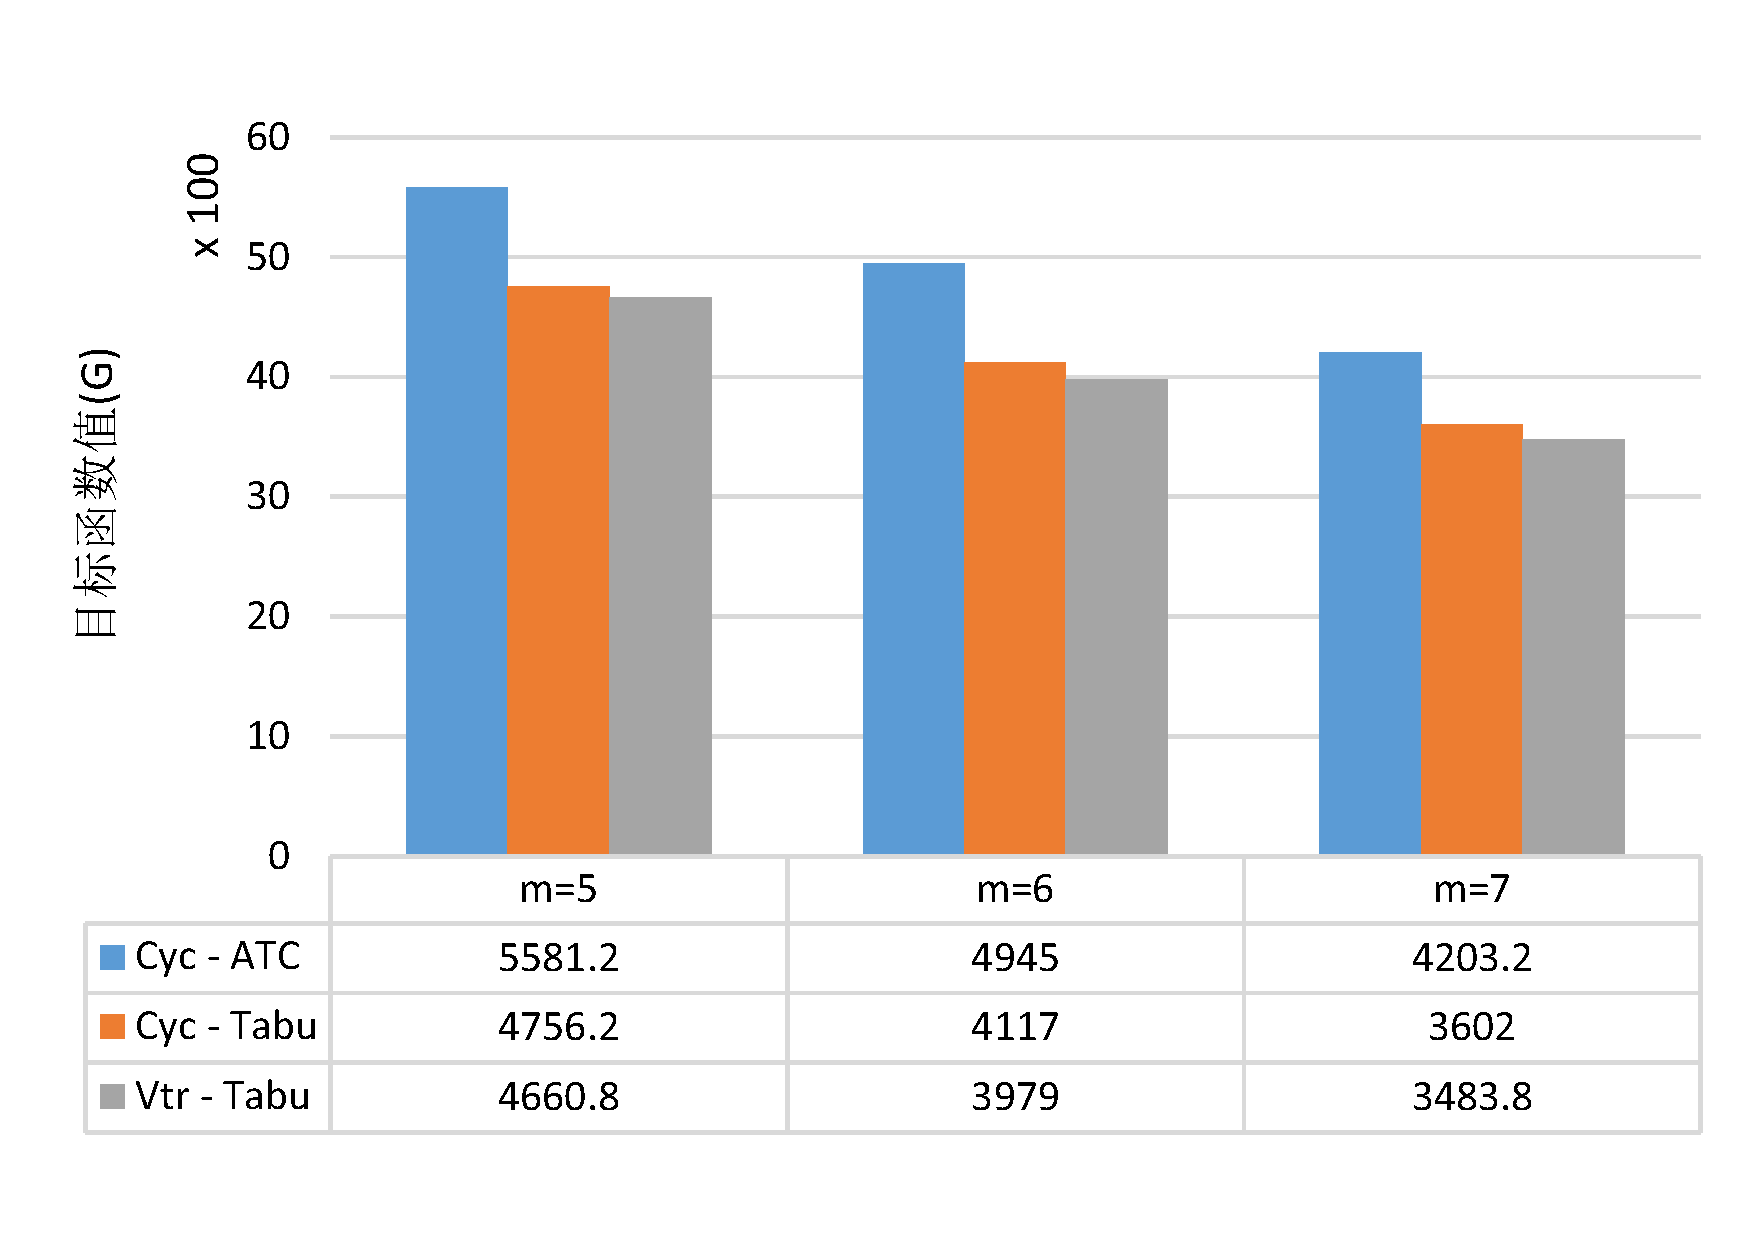
\includegraphics[height = 6cm, angle = -90]{basic_04_20}}
\subfloat[$n = 30$]{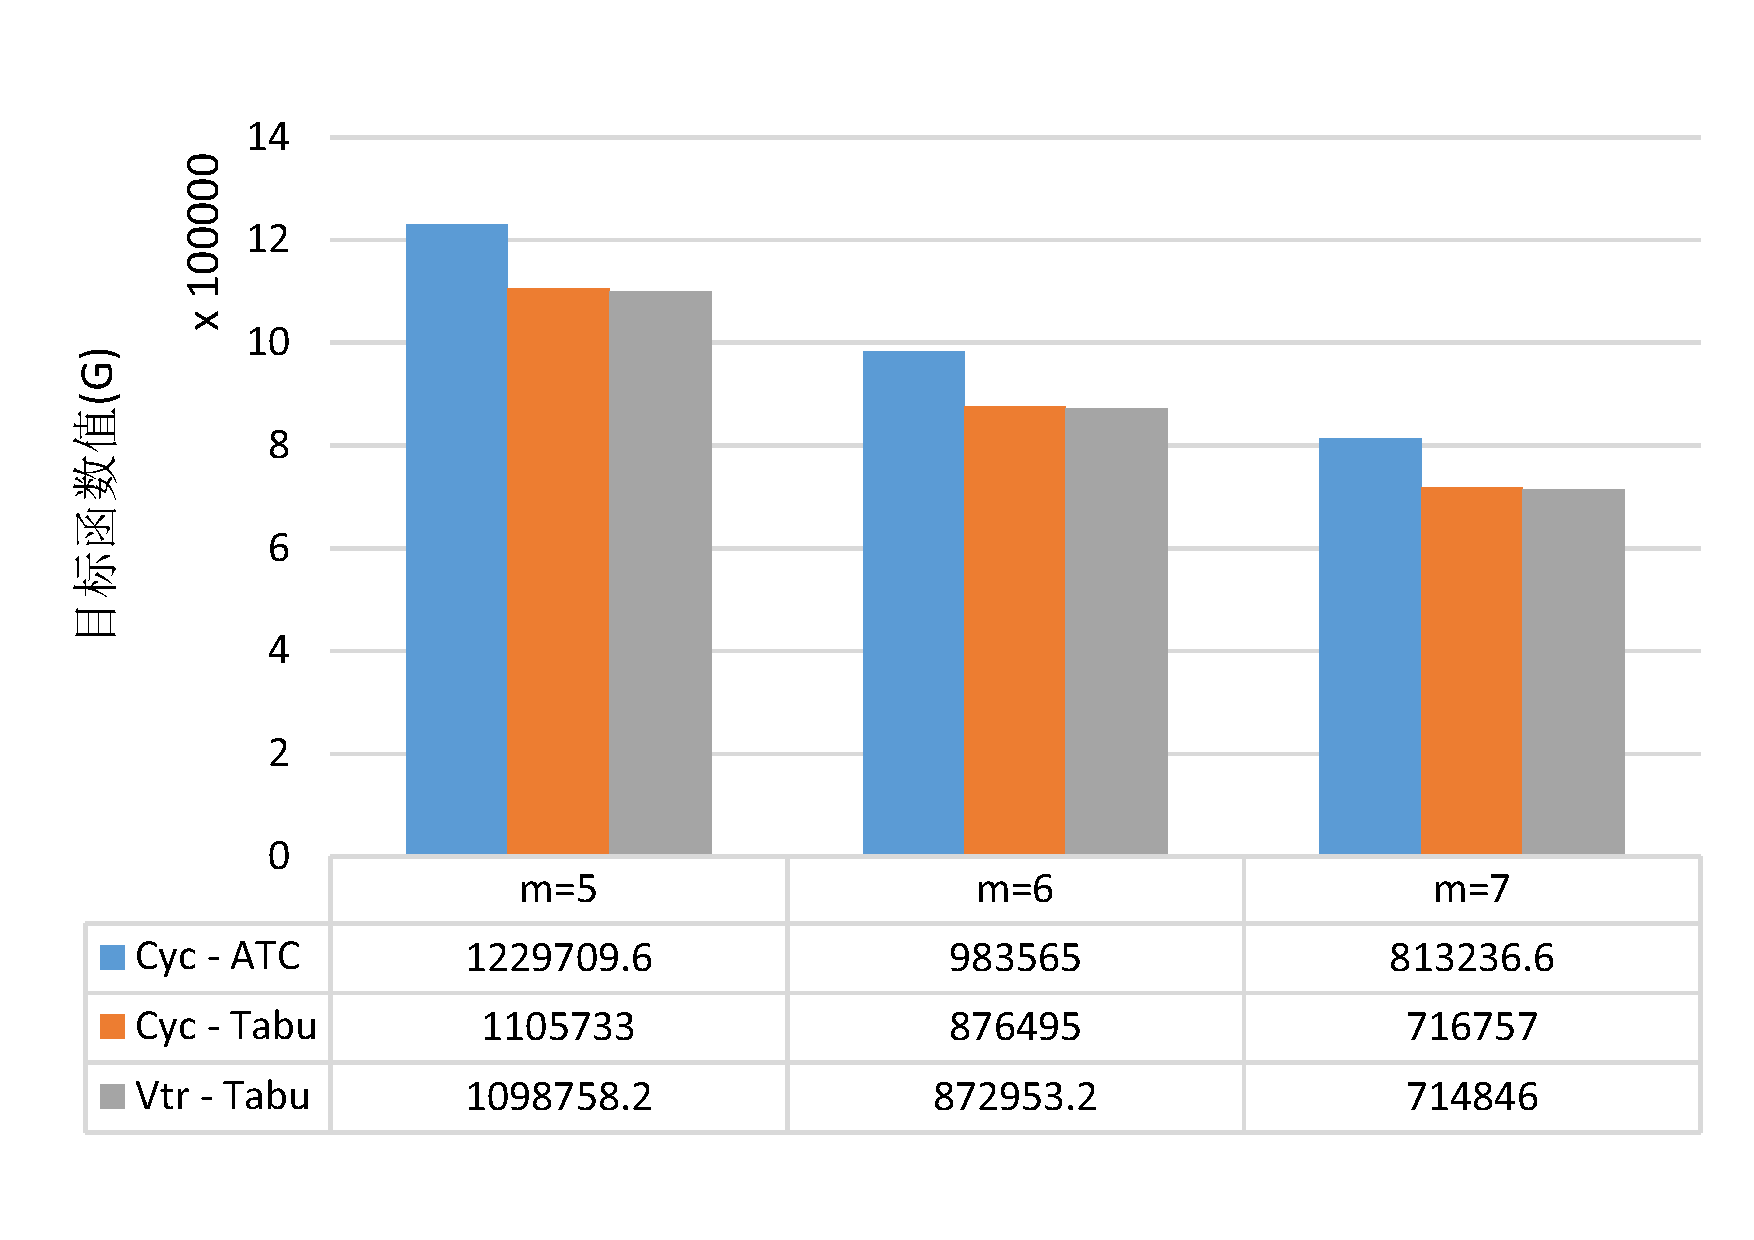
\includegraphics[height = 6cm, angle = -90]{basic_04_300}}
\subfloat[$n = 50$]{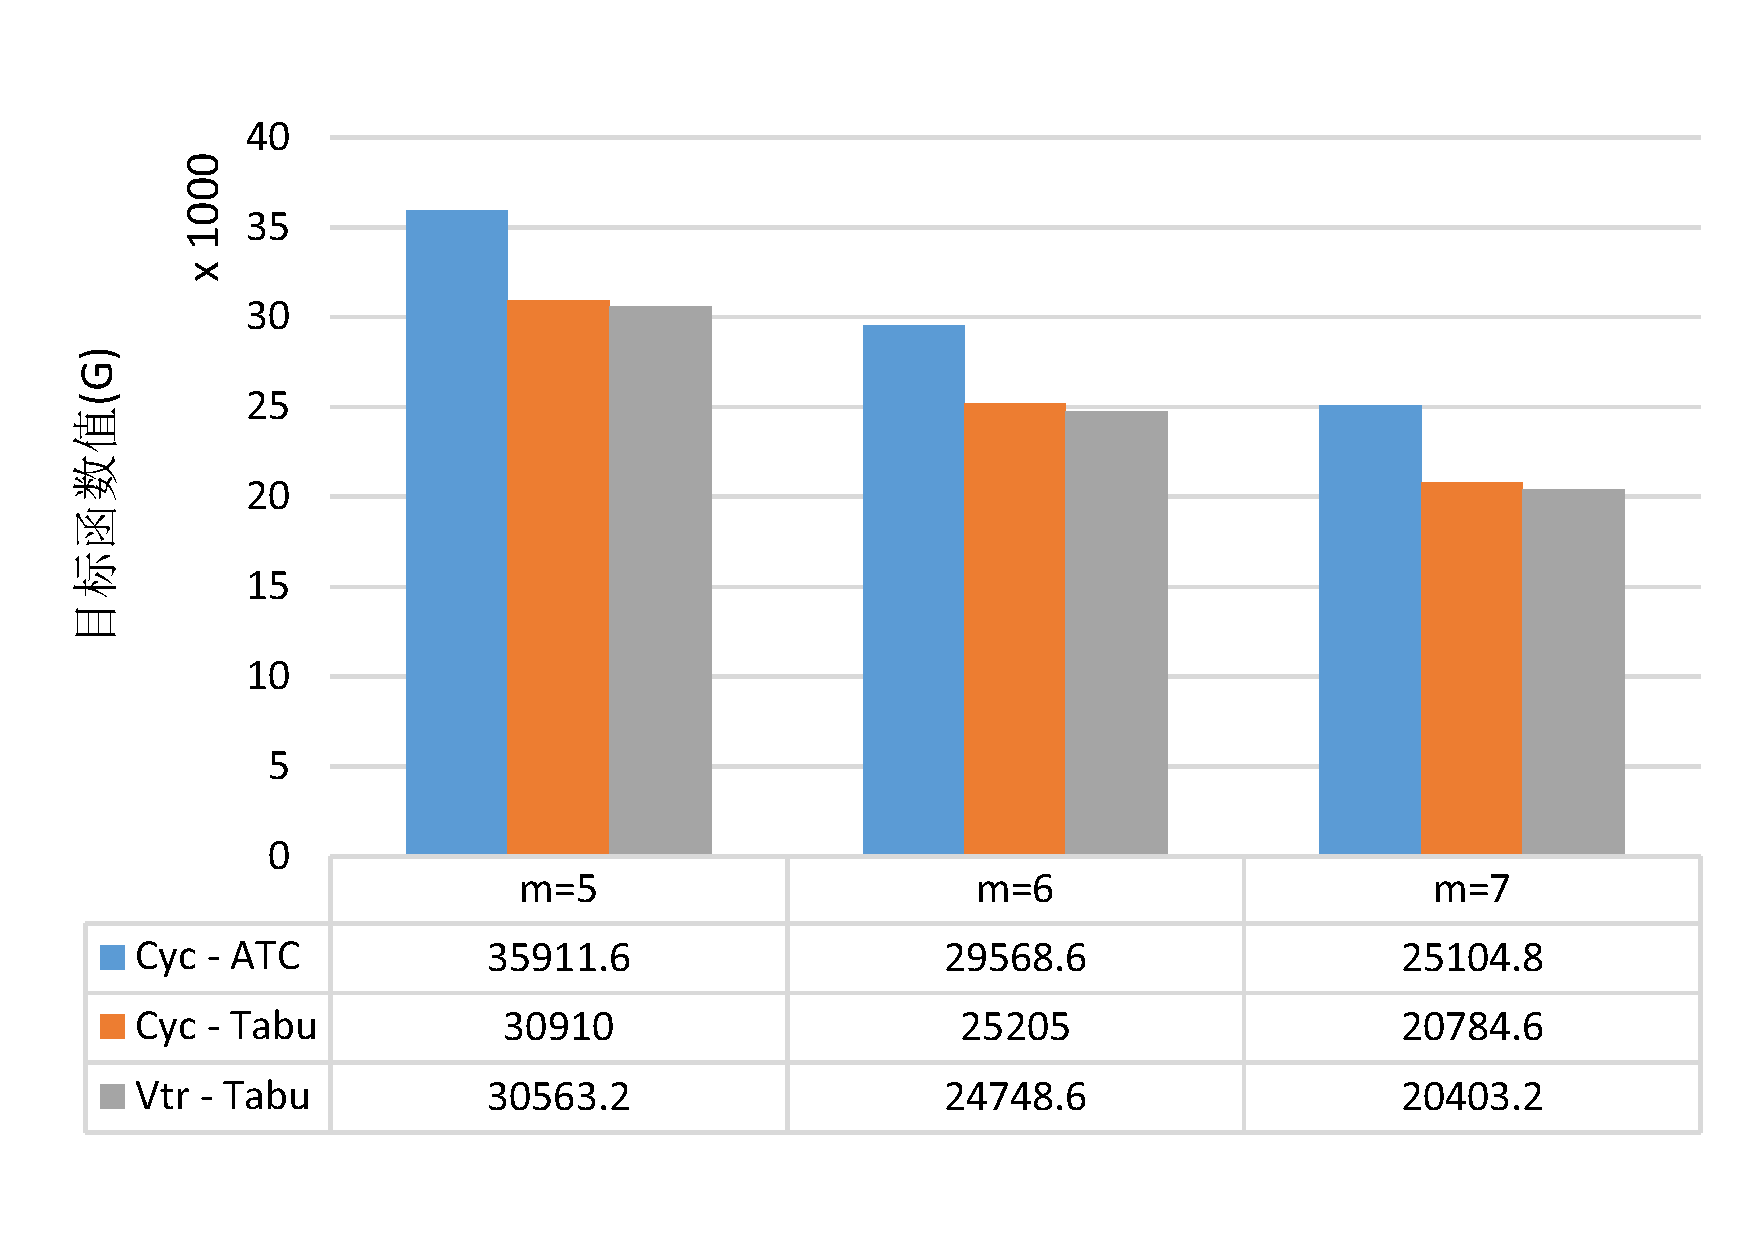
\includegraphics[height = 6cm, angle = -90]{basic_04_50}}
\subfloat[$n = 70$]{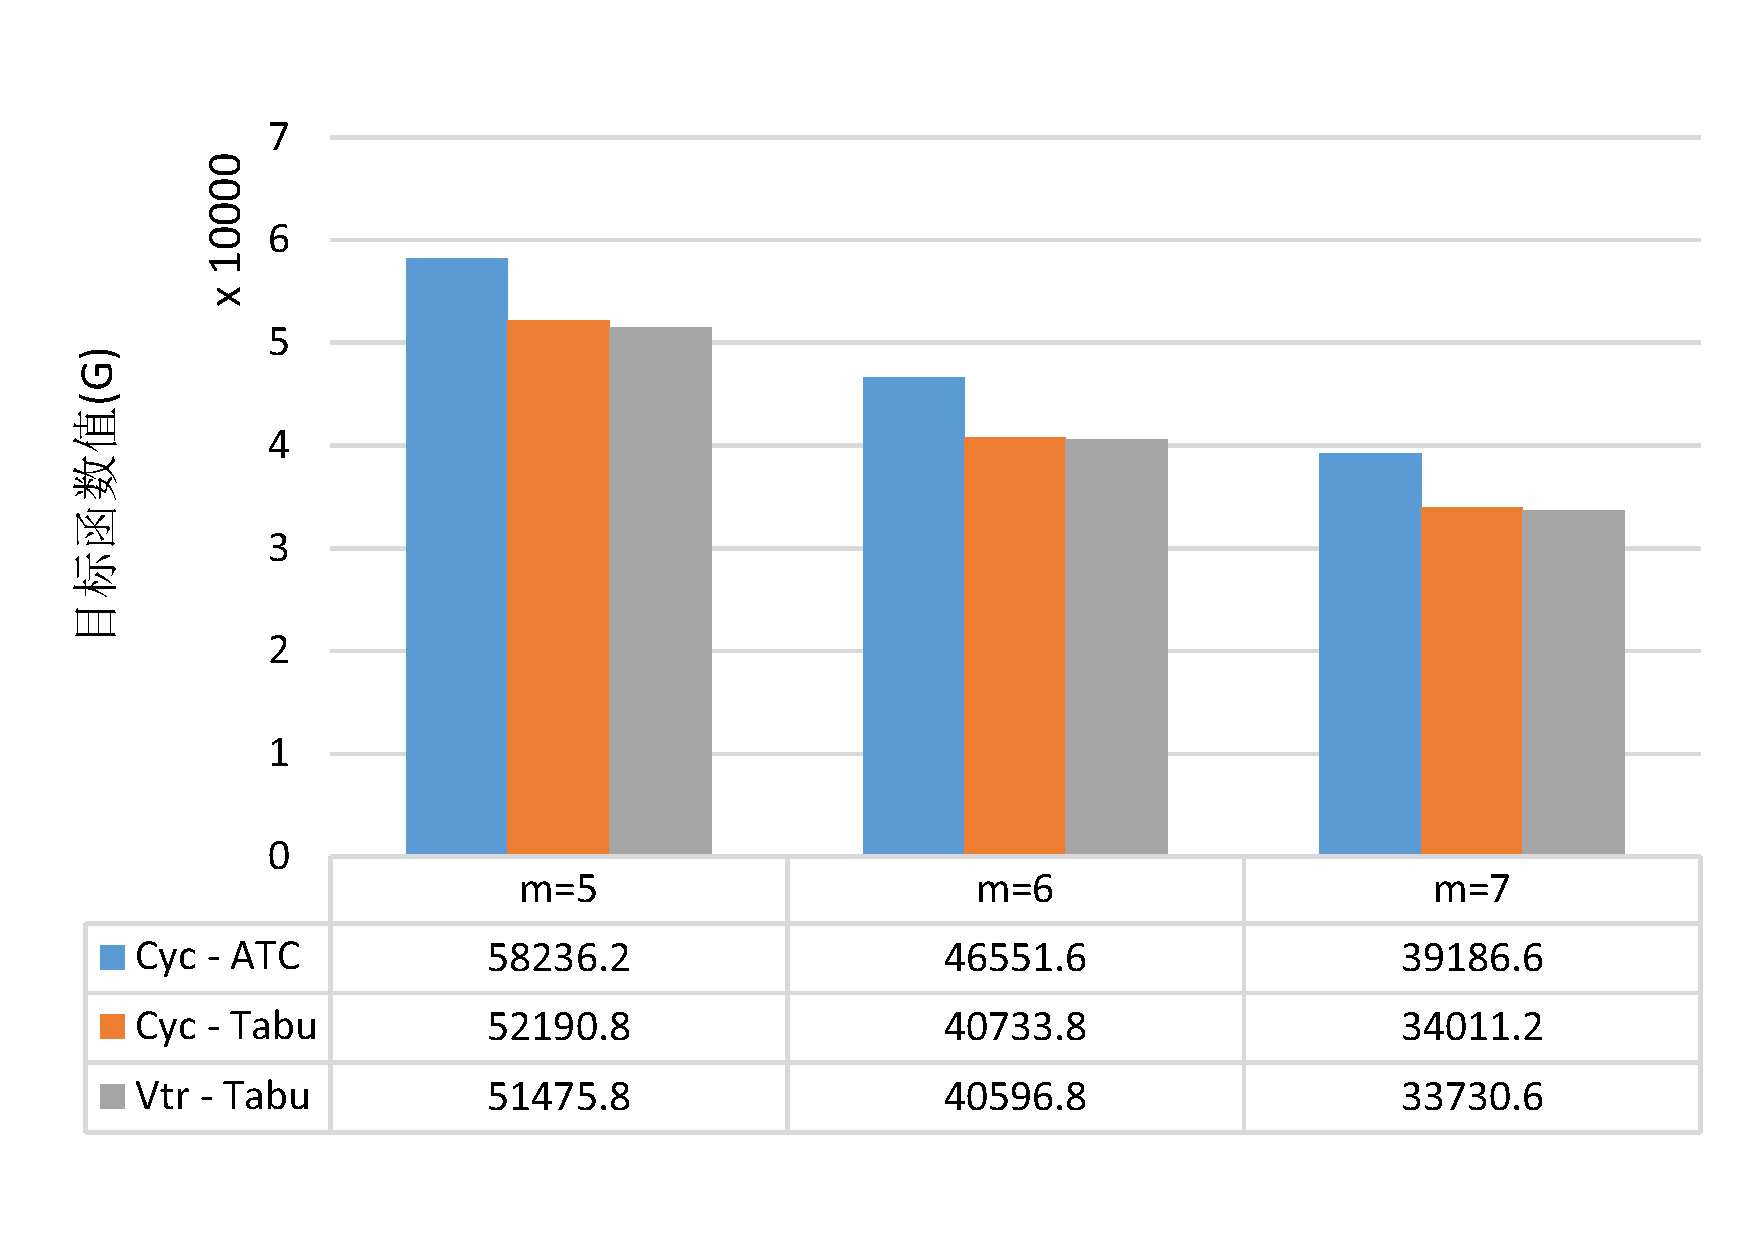
\includegraphics[height = 6cm, angle = -90]{basic_04_70}}\\
\subfloat[$n = 100$]{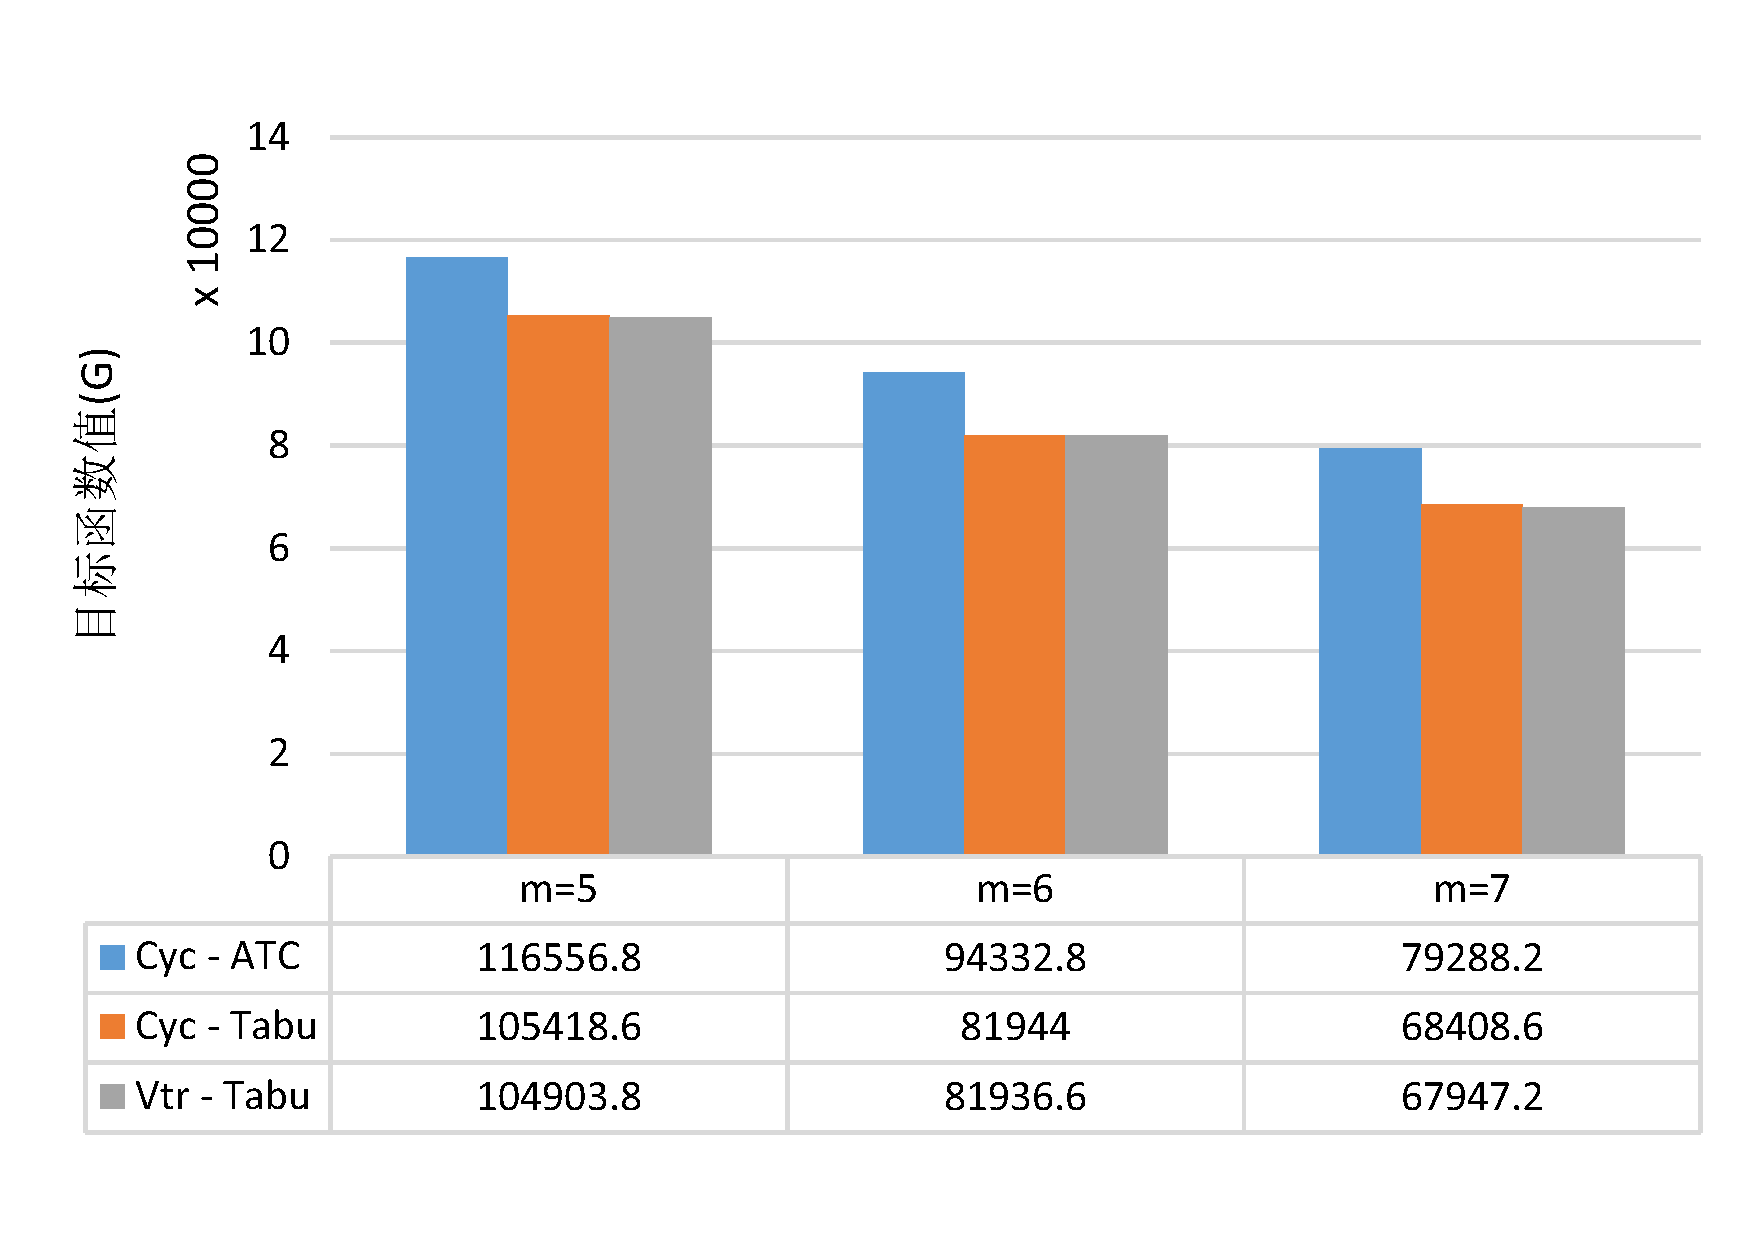
\includegraphics[height = 6cm, angle = -90]{basic_04_100}}
\subfloat[$n = 150$]{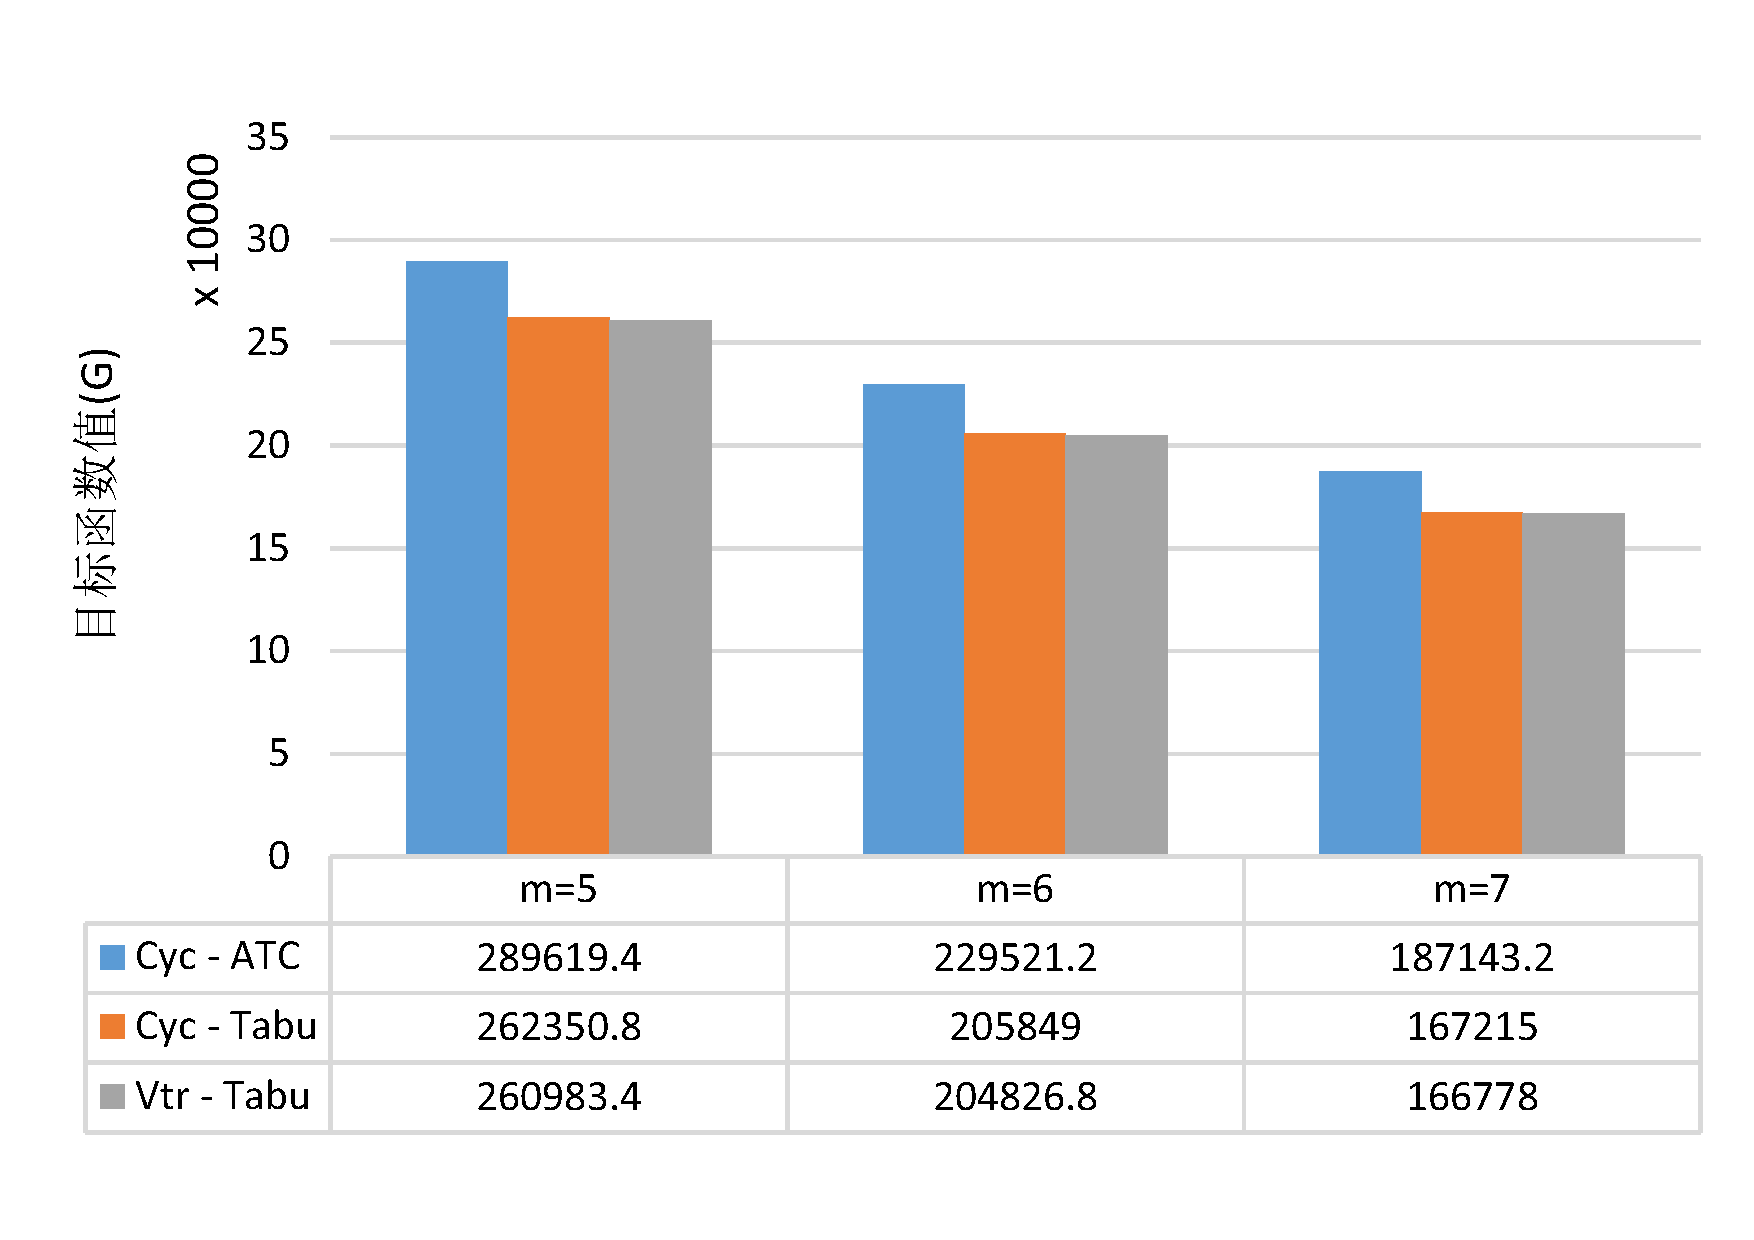
\includegraphics[height = 6cm, angle = -90]{basic_04_150}}
\subfloat[$n = 200$]{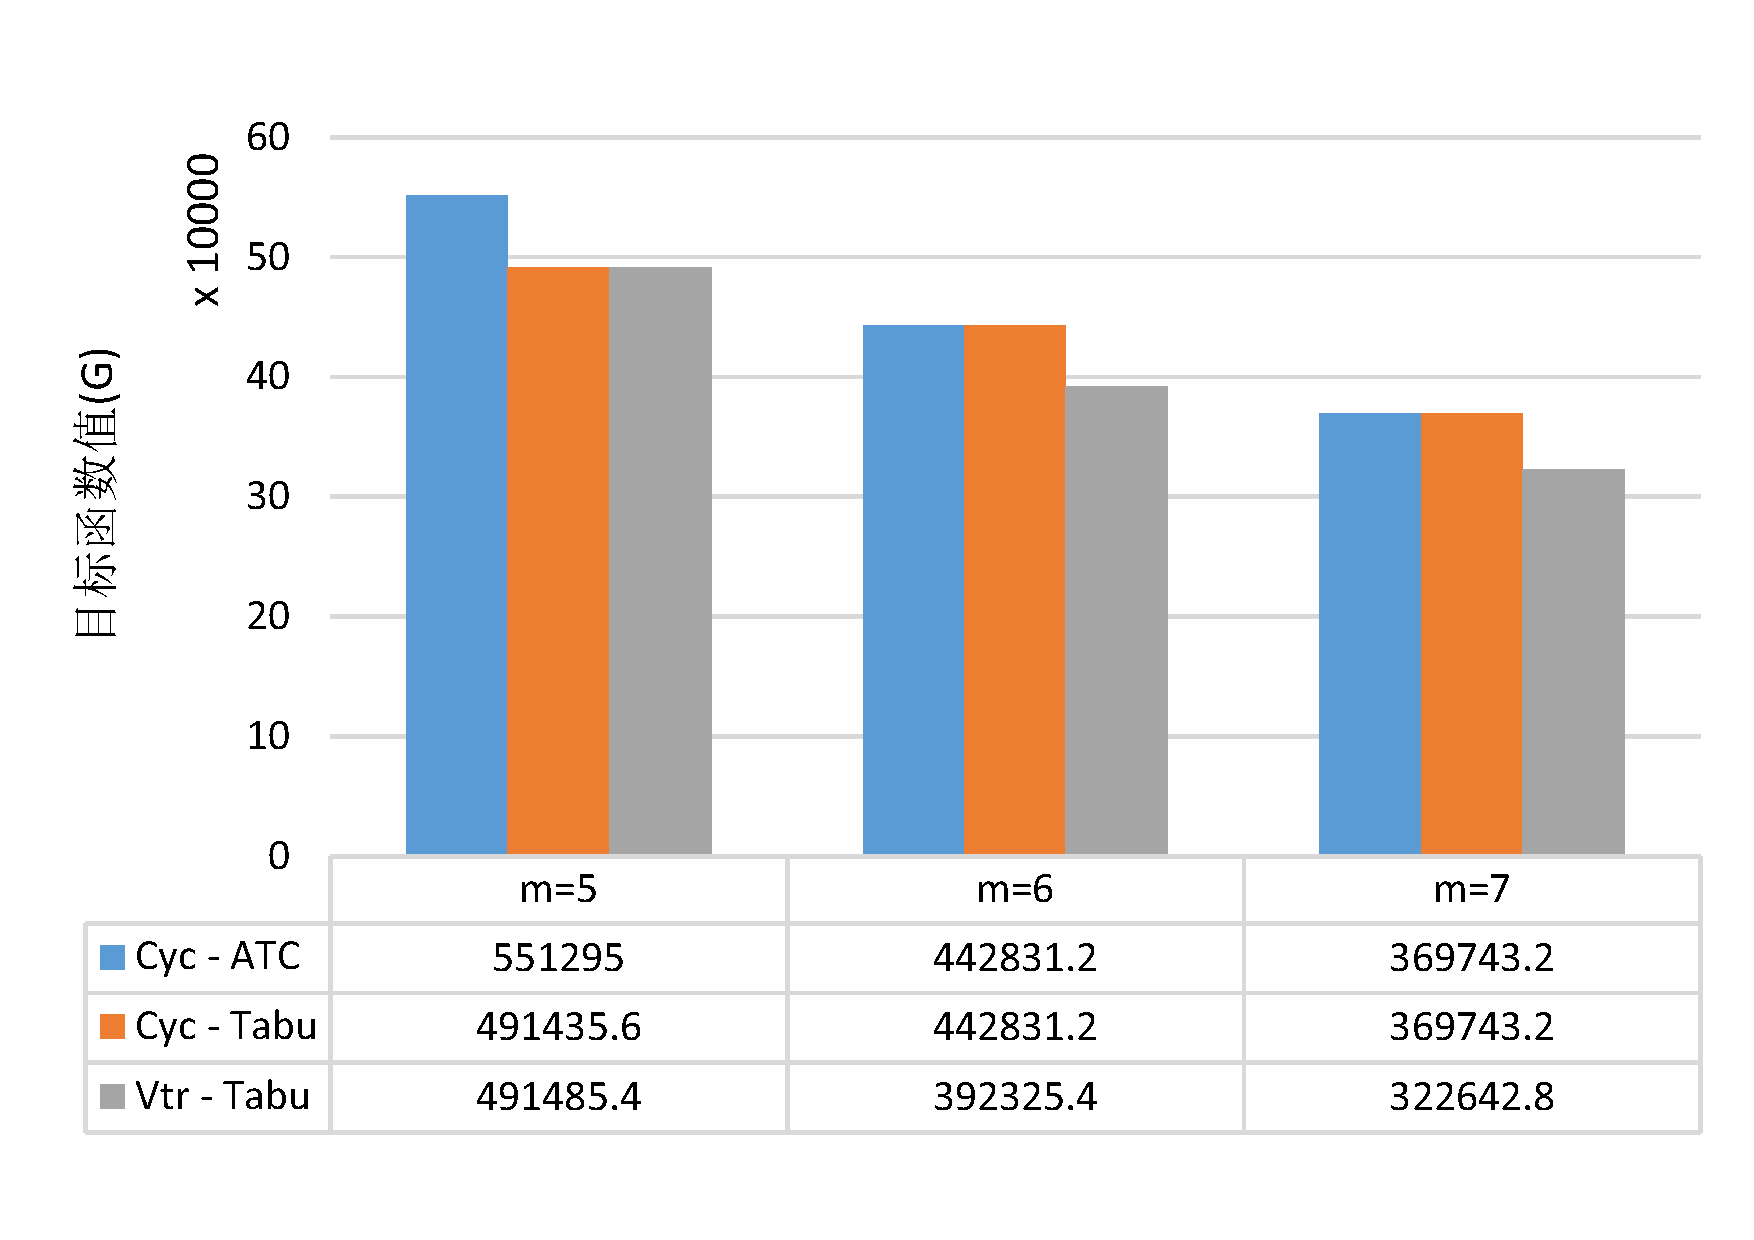
\includegraphics[height = 6cm, angle = -90]{basic_04_200}}
\subfloat[$n = 300$]{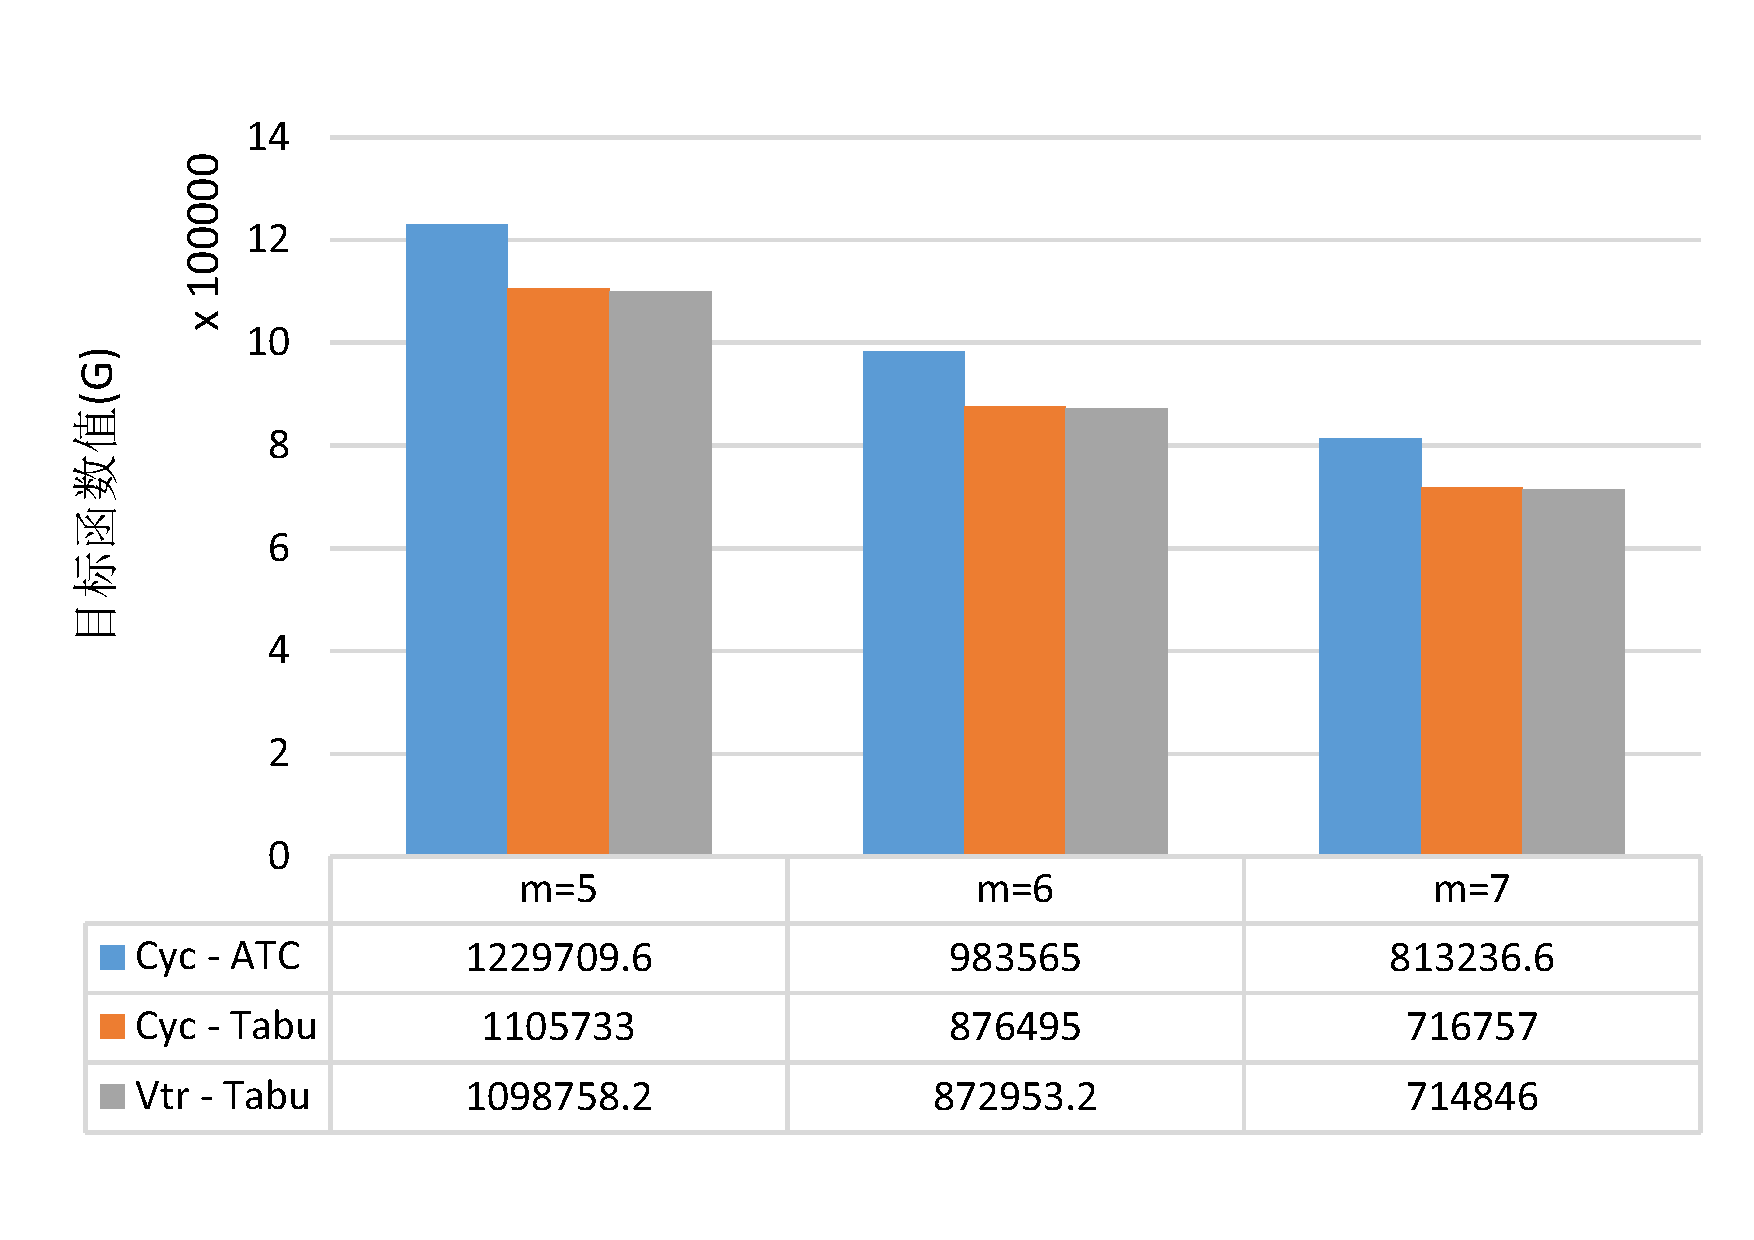
\includegraphics[height = 6cm, angle = -90]{basic_04_300}}\\
\subfloat[$n = 500$]{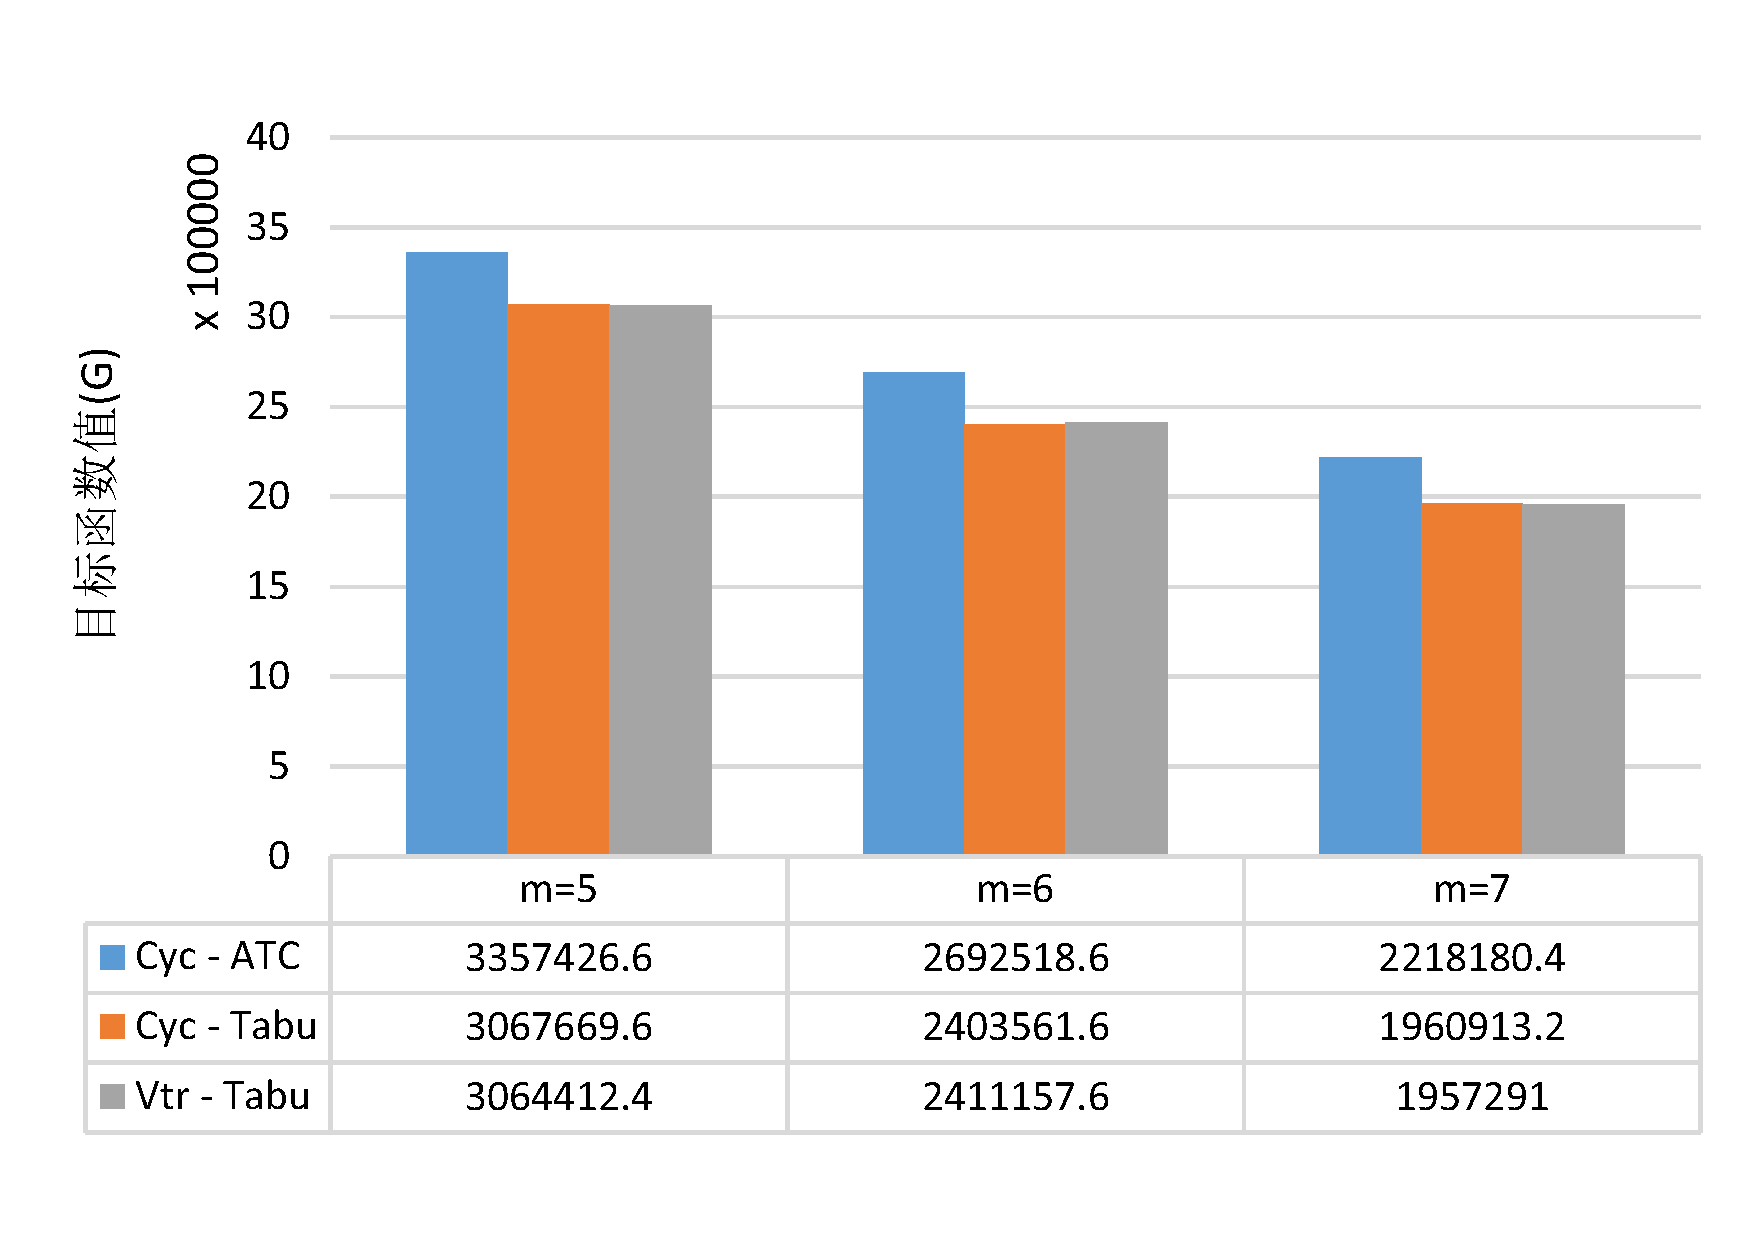
\includegraphics[height = 6cm, angle = -90]{basic_04_500}}
\subfloat[$n = 750$]{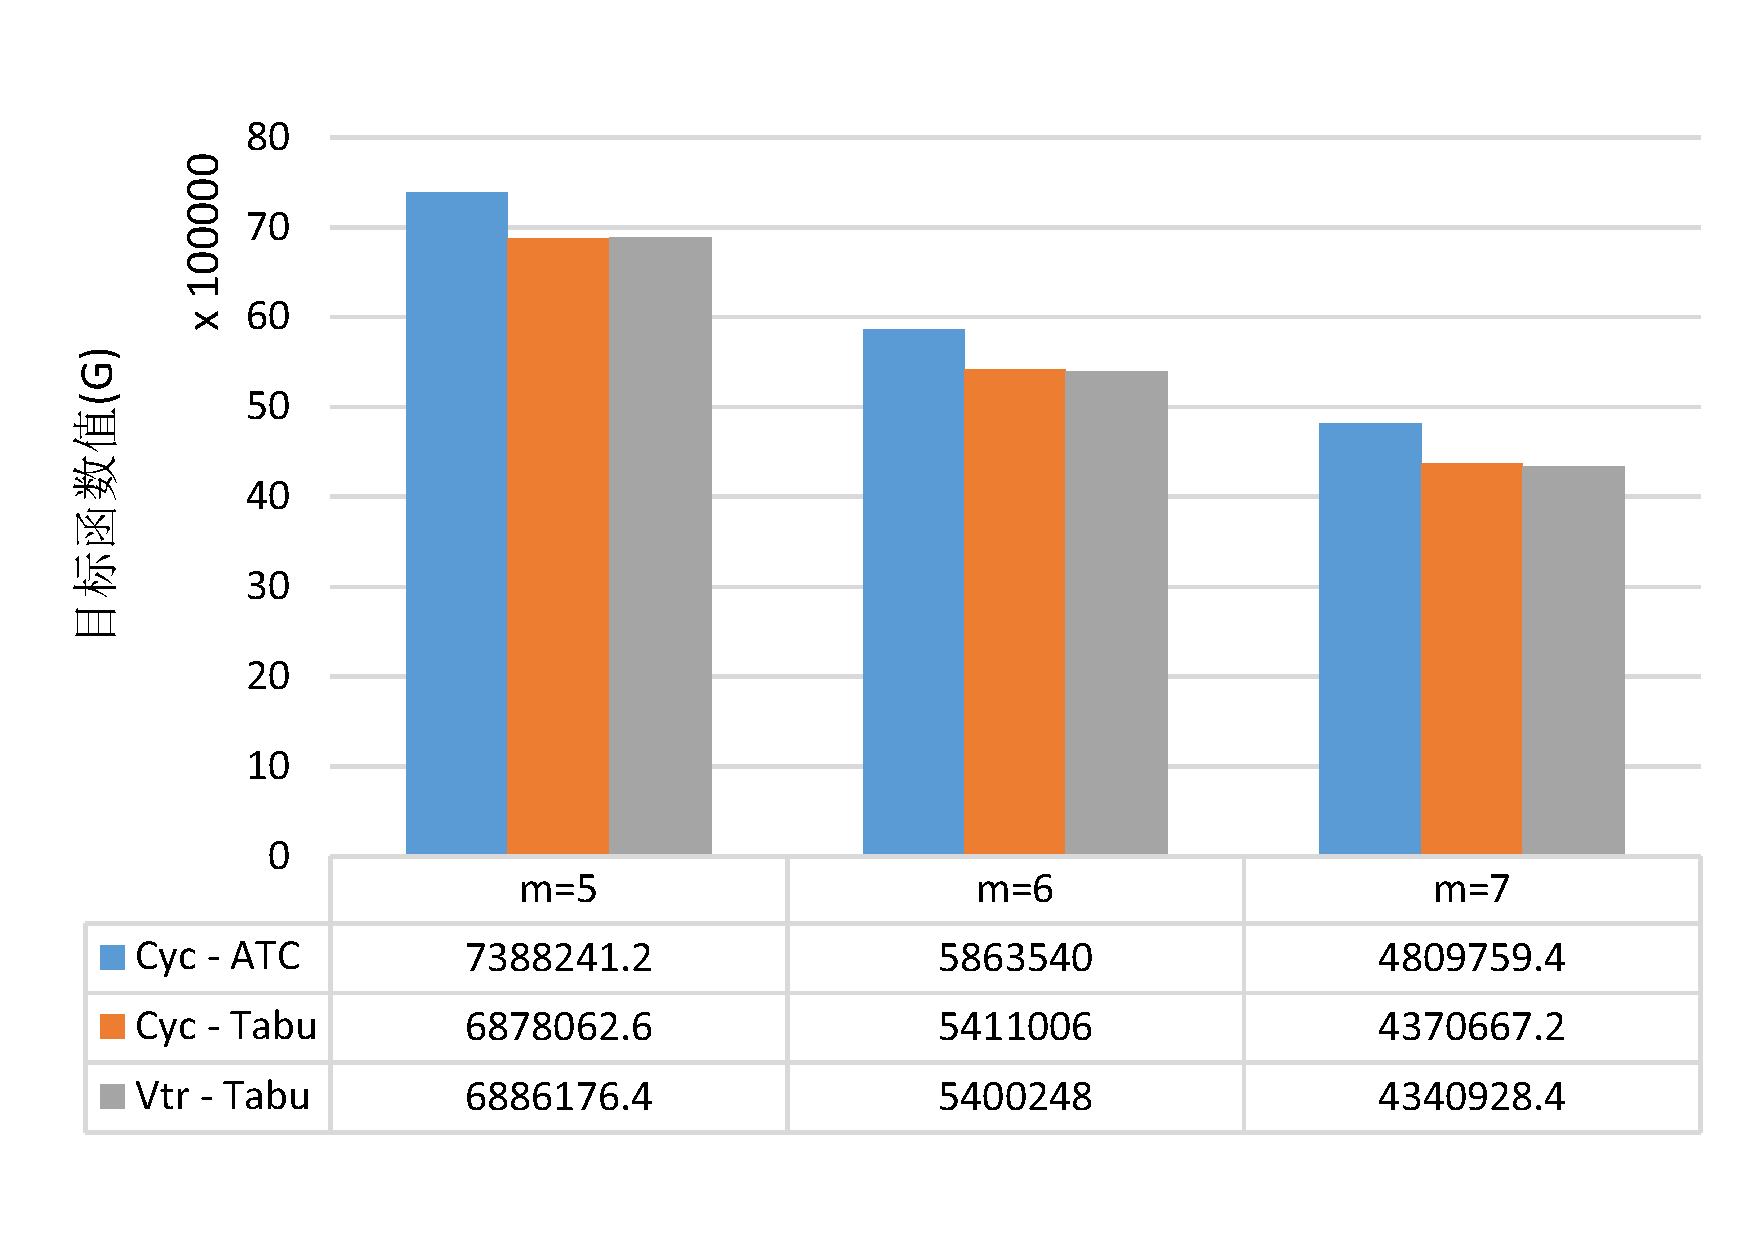
\includegraphics[height = 6cm, angle = -90]{basic_04_750}}
\subfloat[$n = 1000$]{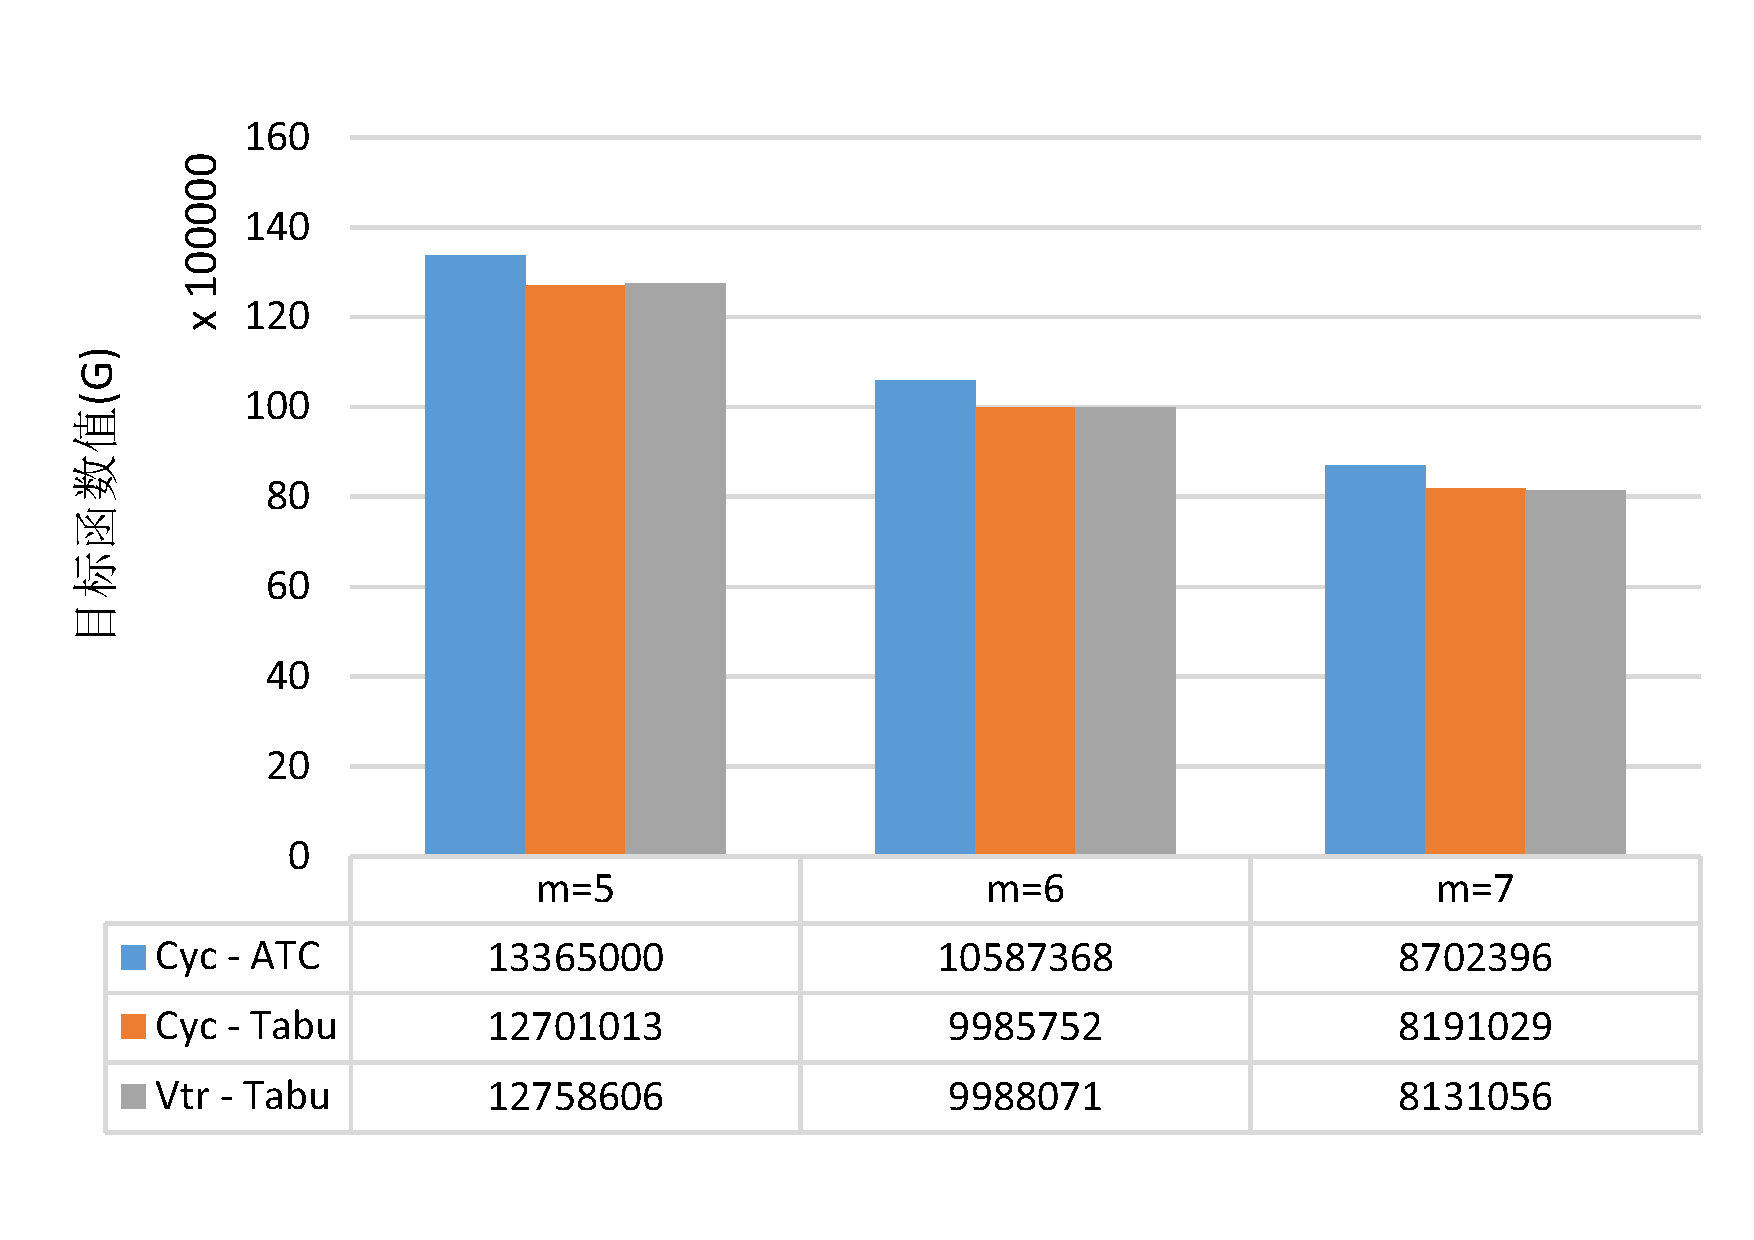
\includegraphics[height = 6cm, angle = -90]{basic_04_1000}}
\caption{\label{fig:result1}模型$1$的Cyc -- ATC、Cyc -- Tabu、Vtr -- Tabu 算法求解目标函数值比较$(\lambda_1 = 0.4)$}
\end{sidewaysfigure}

\begin{sidewaysfigure}
\centering
\subfloat[$n = 20$]{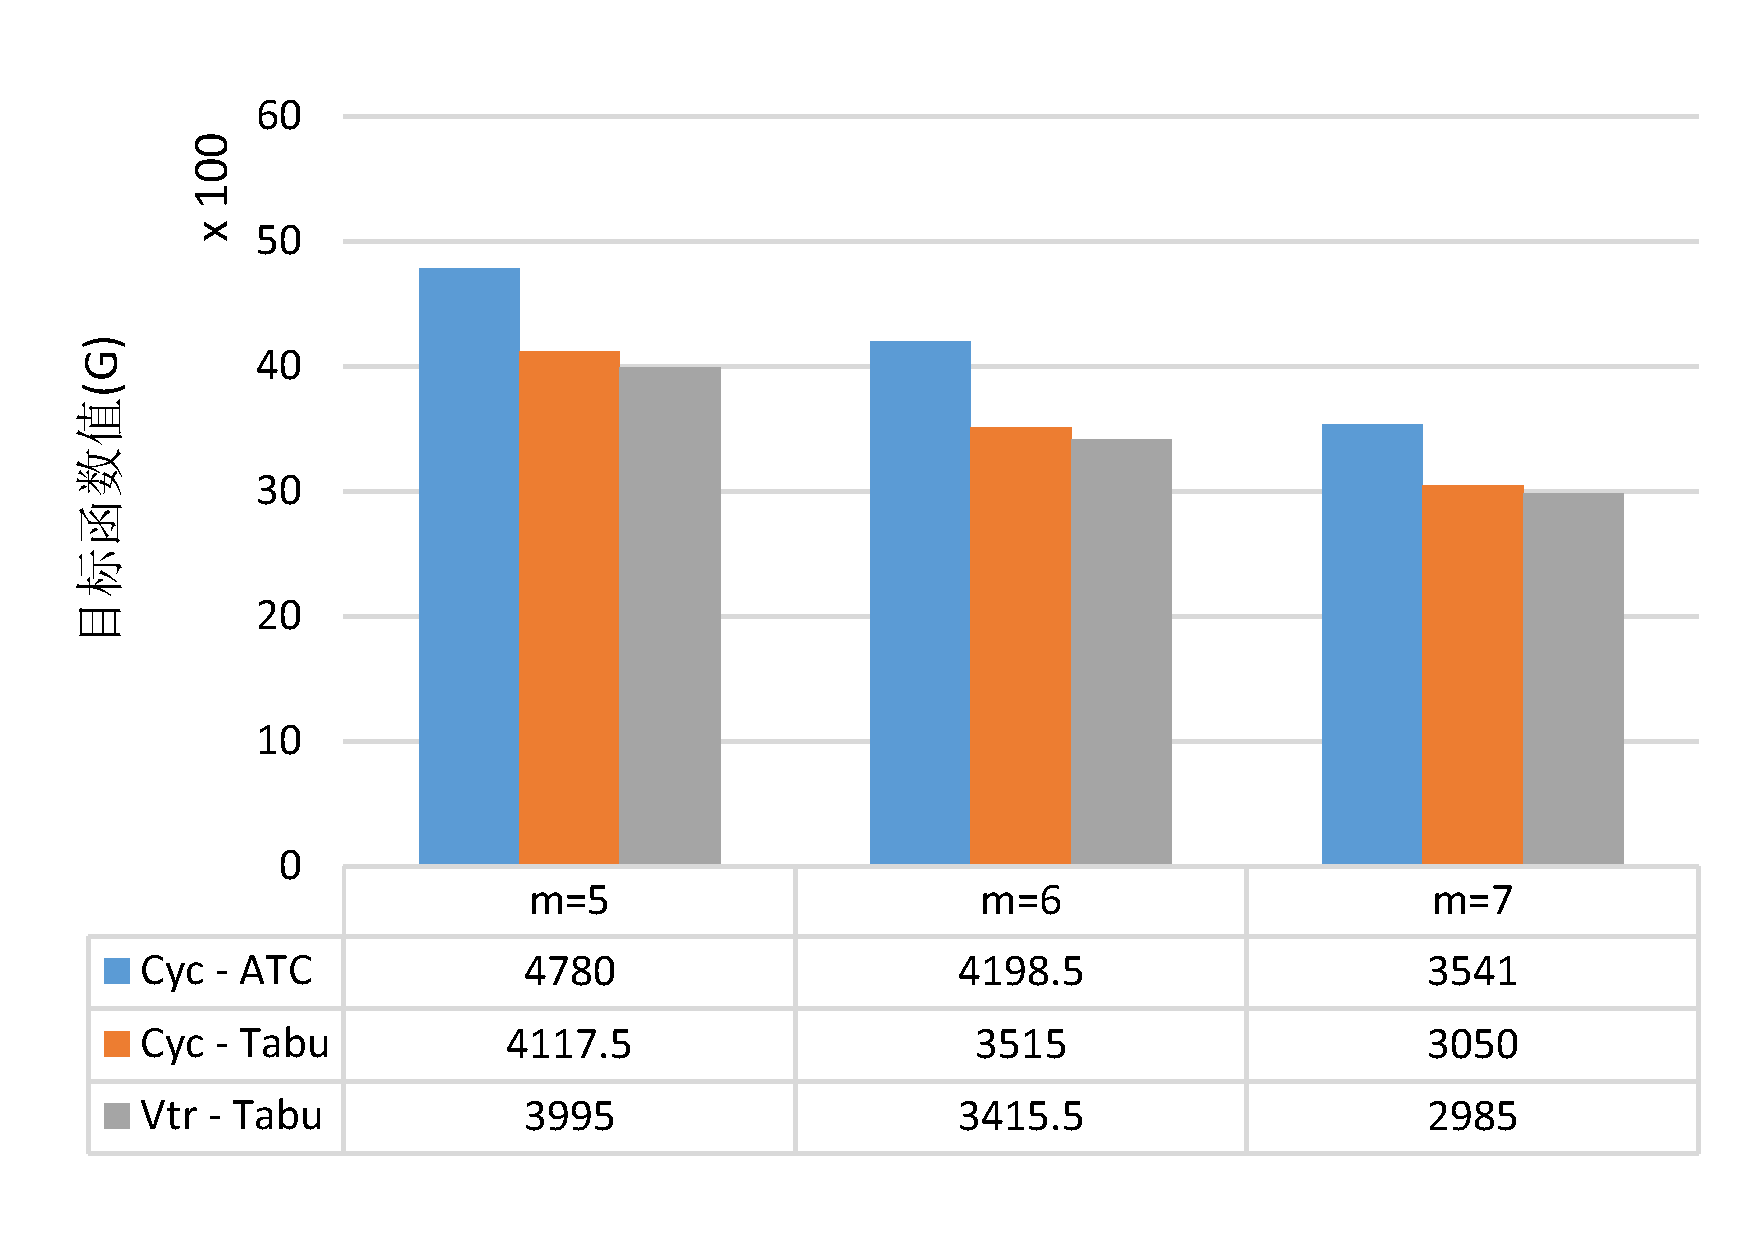
\includegraphics[height = 6cm, angle = -90]{basic_05_20}}
\subfloat[$n = 30$]{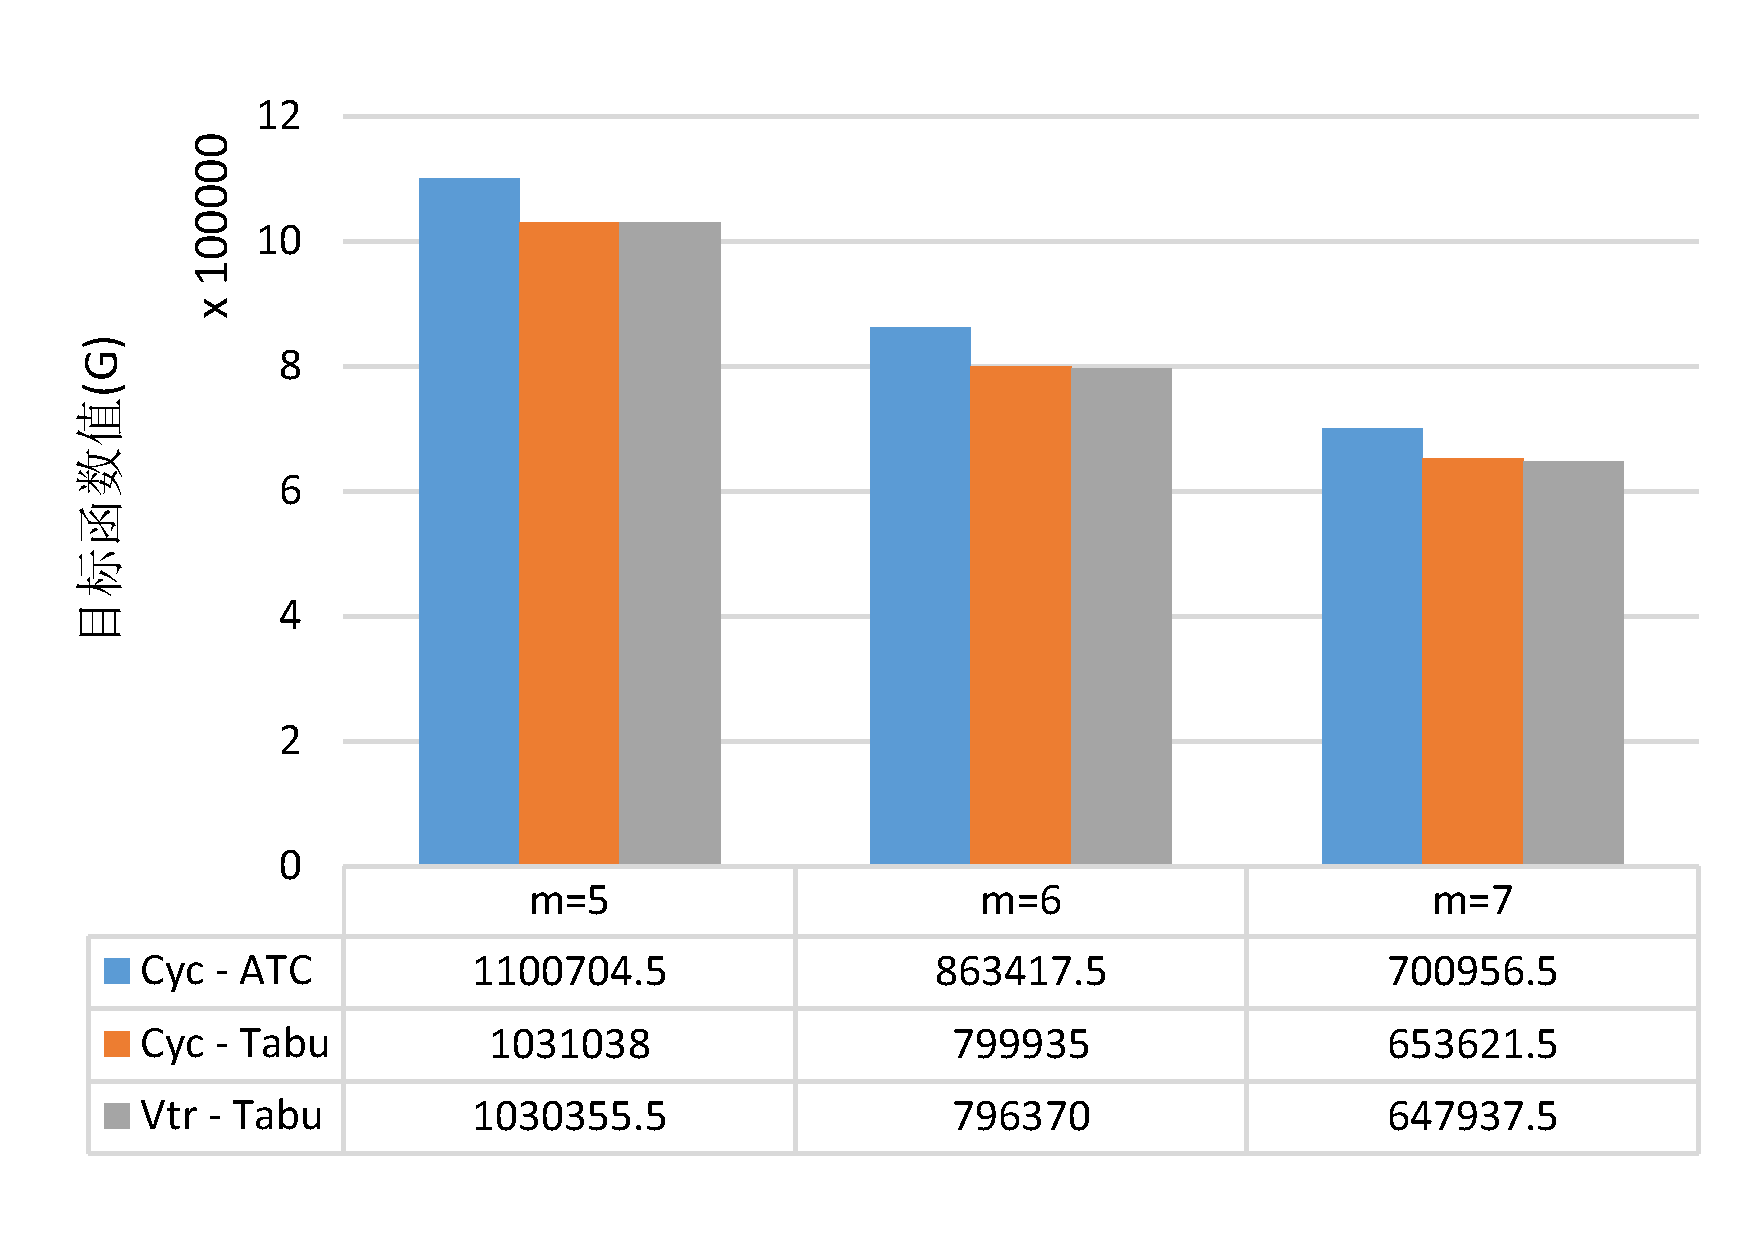
\includegraphics[height = 6cm, angle = -90]{basic_05_300}}
\subfloat[$n = 50$]{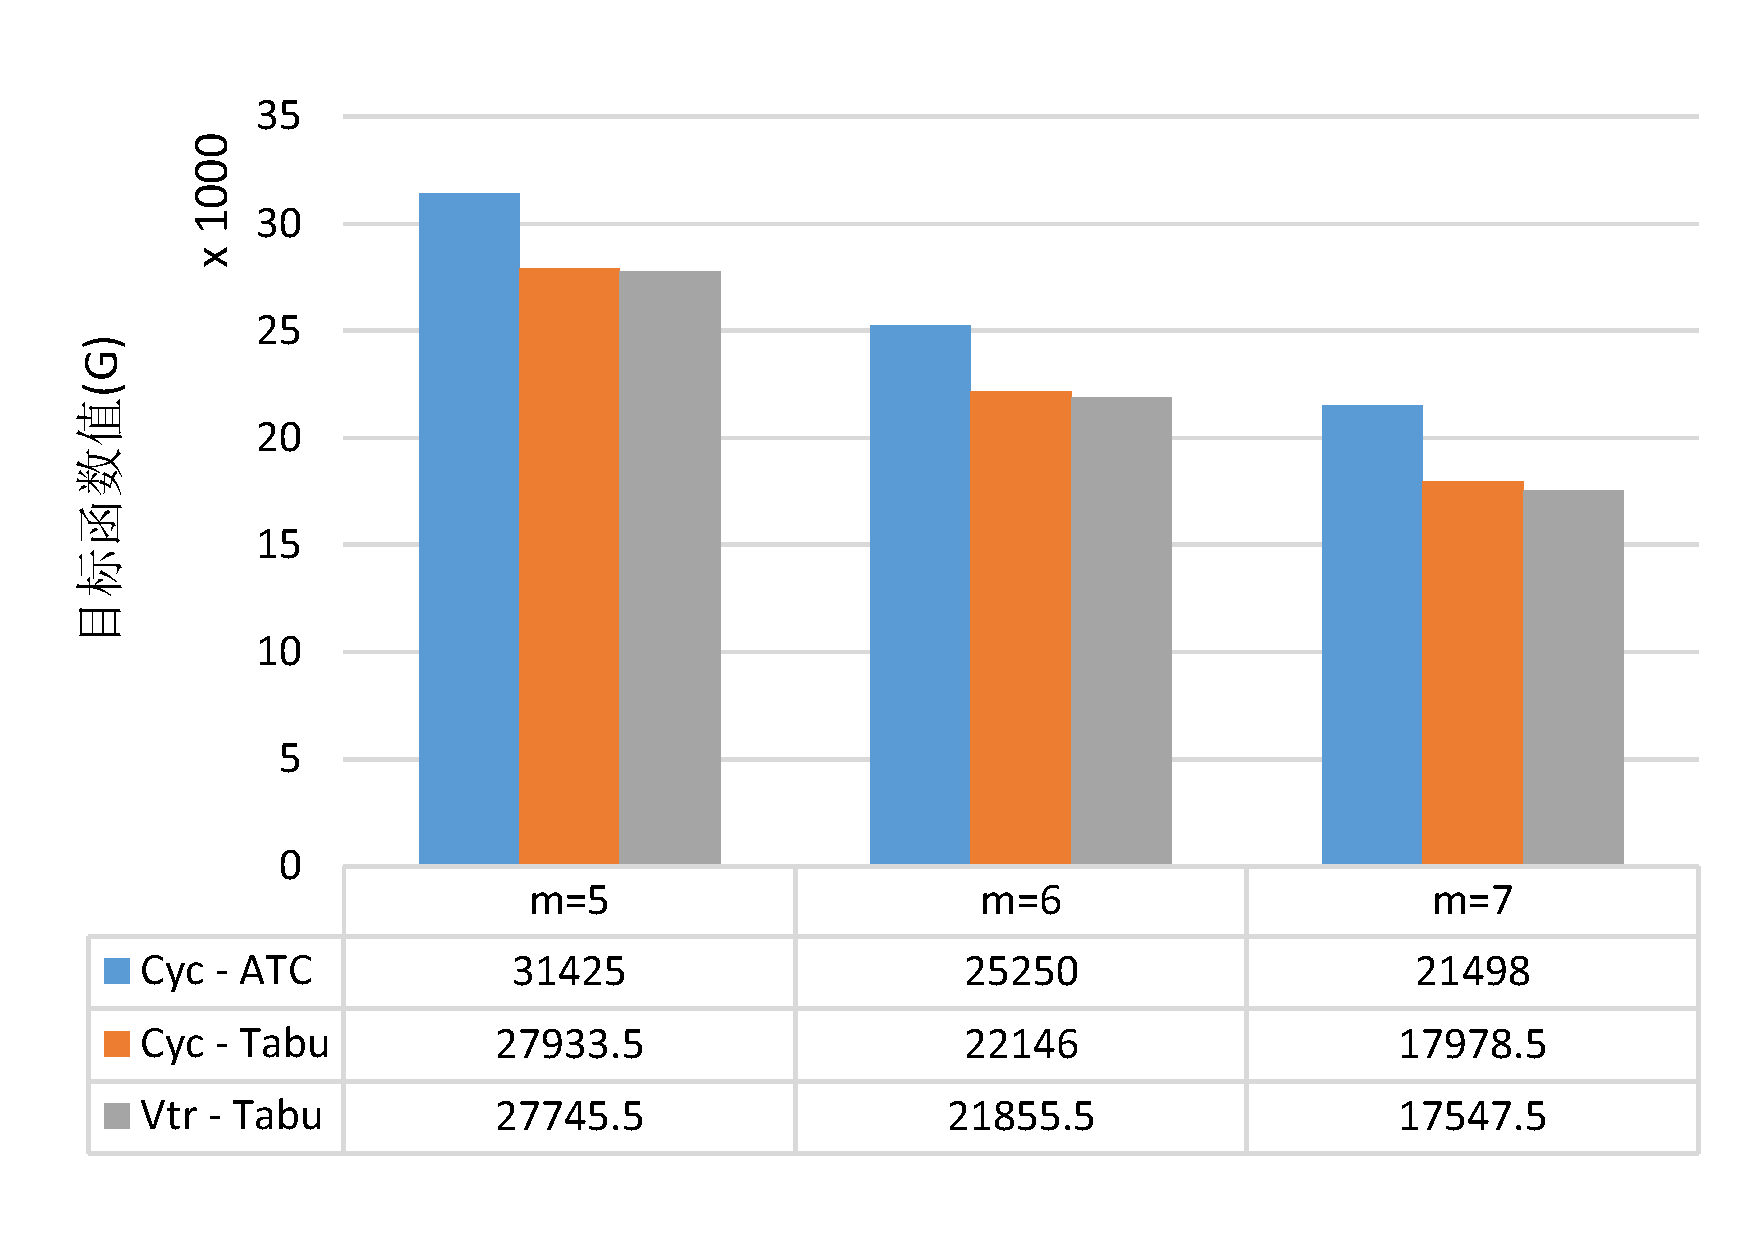
\includegraphics[height = 6cm, angle = -90]{basic_05_50}}
\subfloat[$n = 70$]{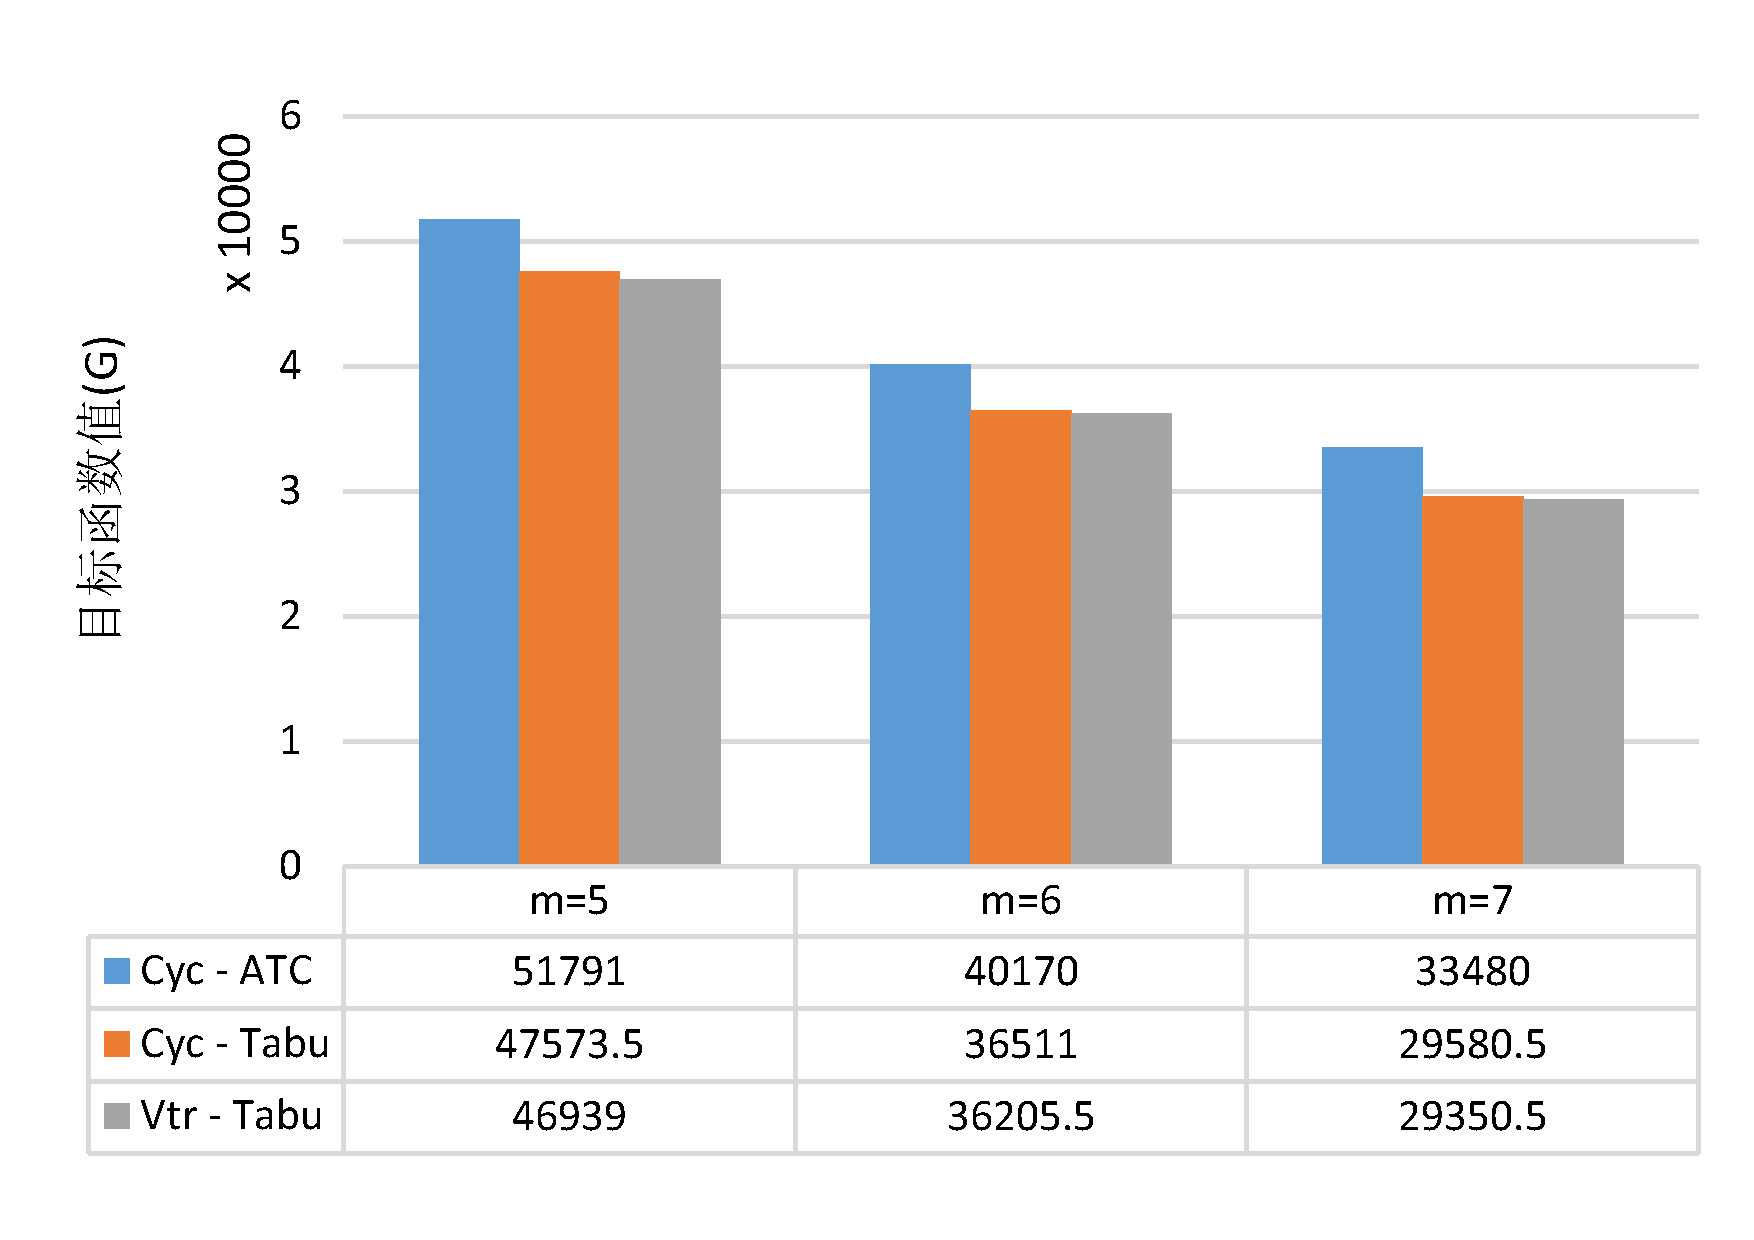
\includegraphics[height = 6cm, angle = -90]{basic_05_70}}\\
\subfloat[$n = 100$]{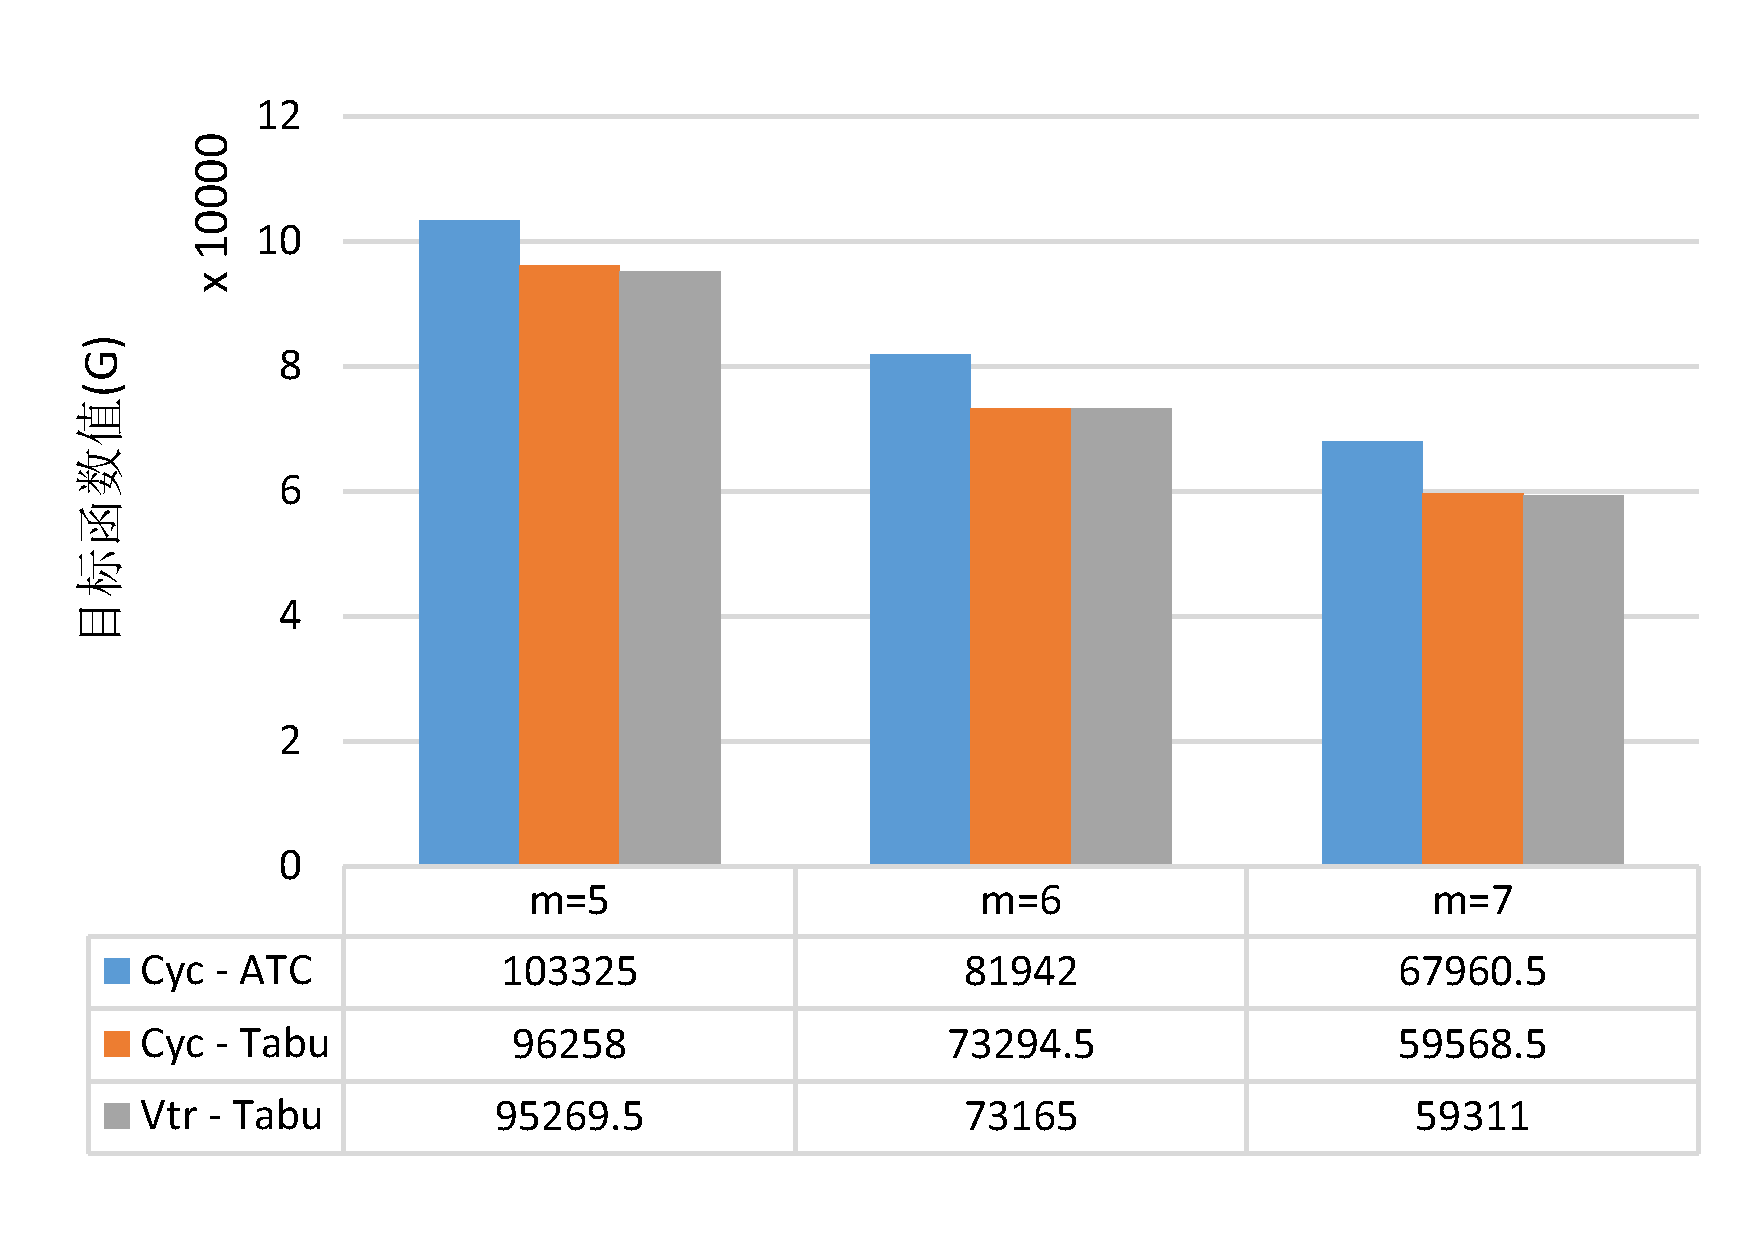
\includegraphics[height = 6cm, angle = -90]{basic_05_100}}
\subfloat[$n = 150$]{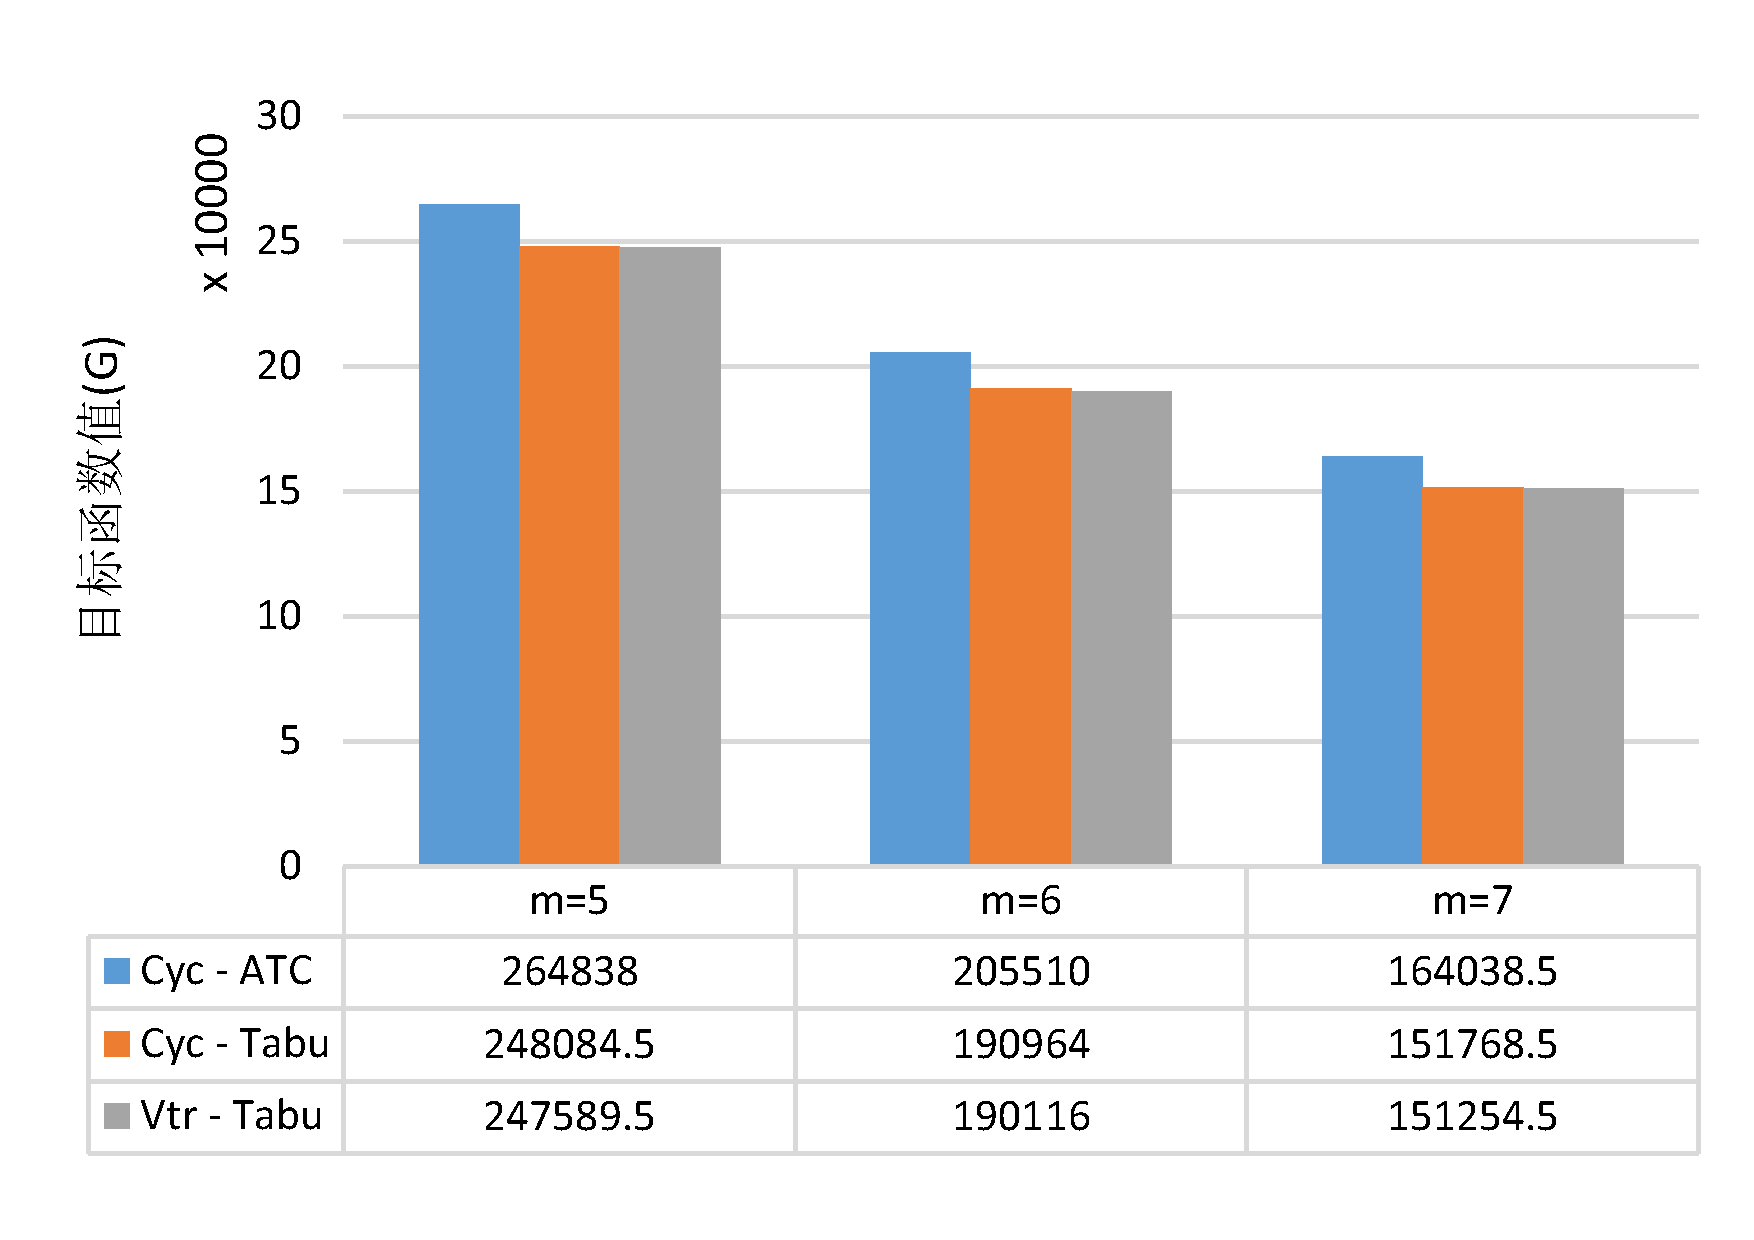
\includegraphics[height = 6cm, angle = -90]{basic_05_150}}
\subfloat[$n = 200$]{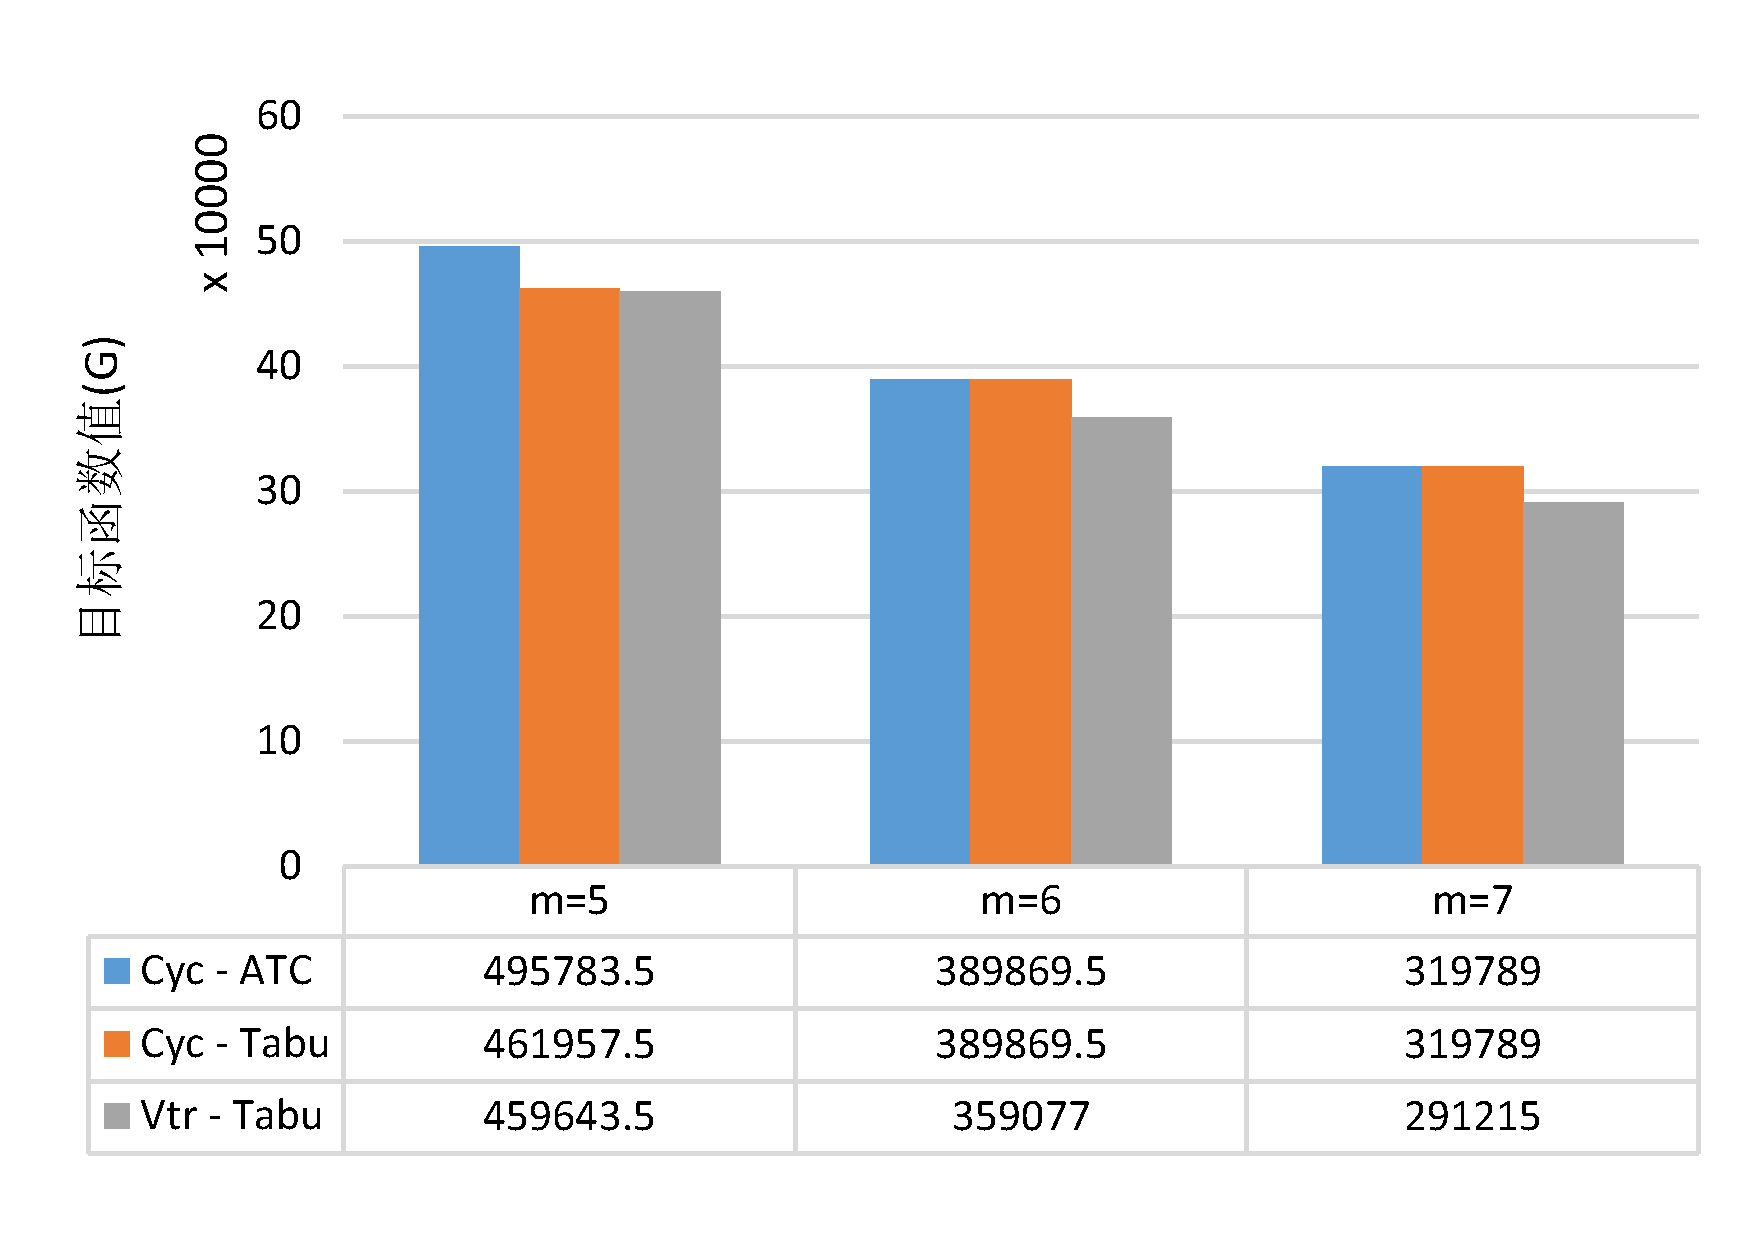
\includegraphics[height = 6cm, angle = -90]{basic_05_200}}
\subfloat[$n = 300$]{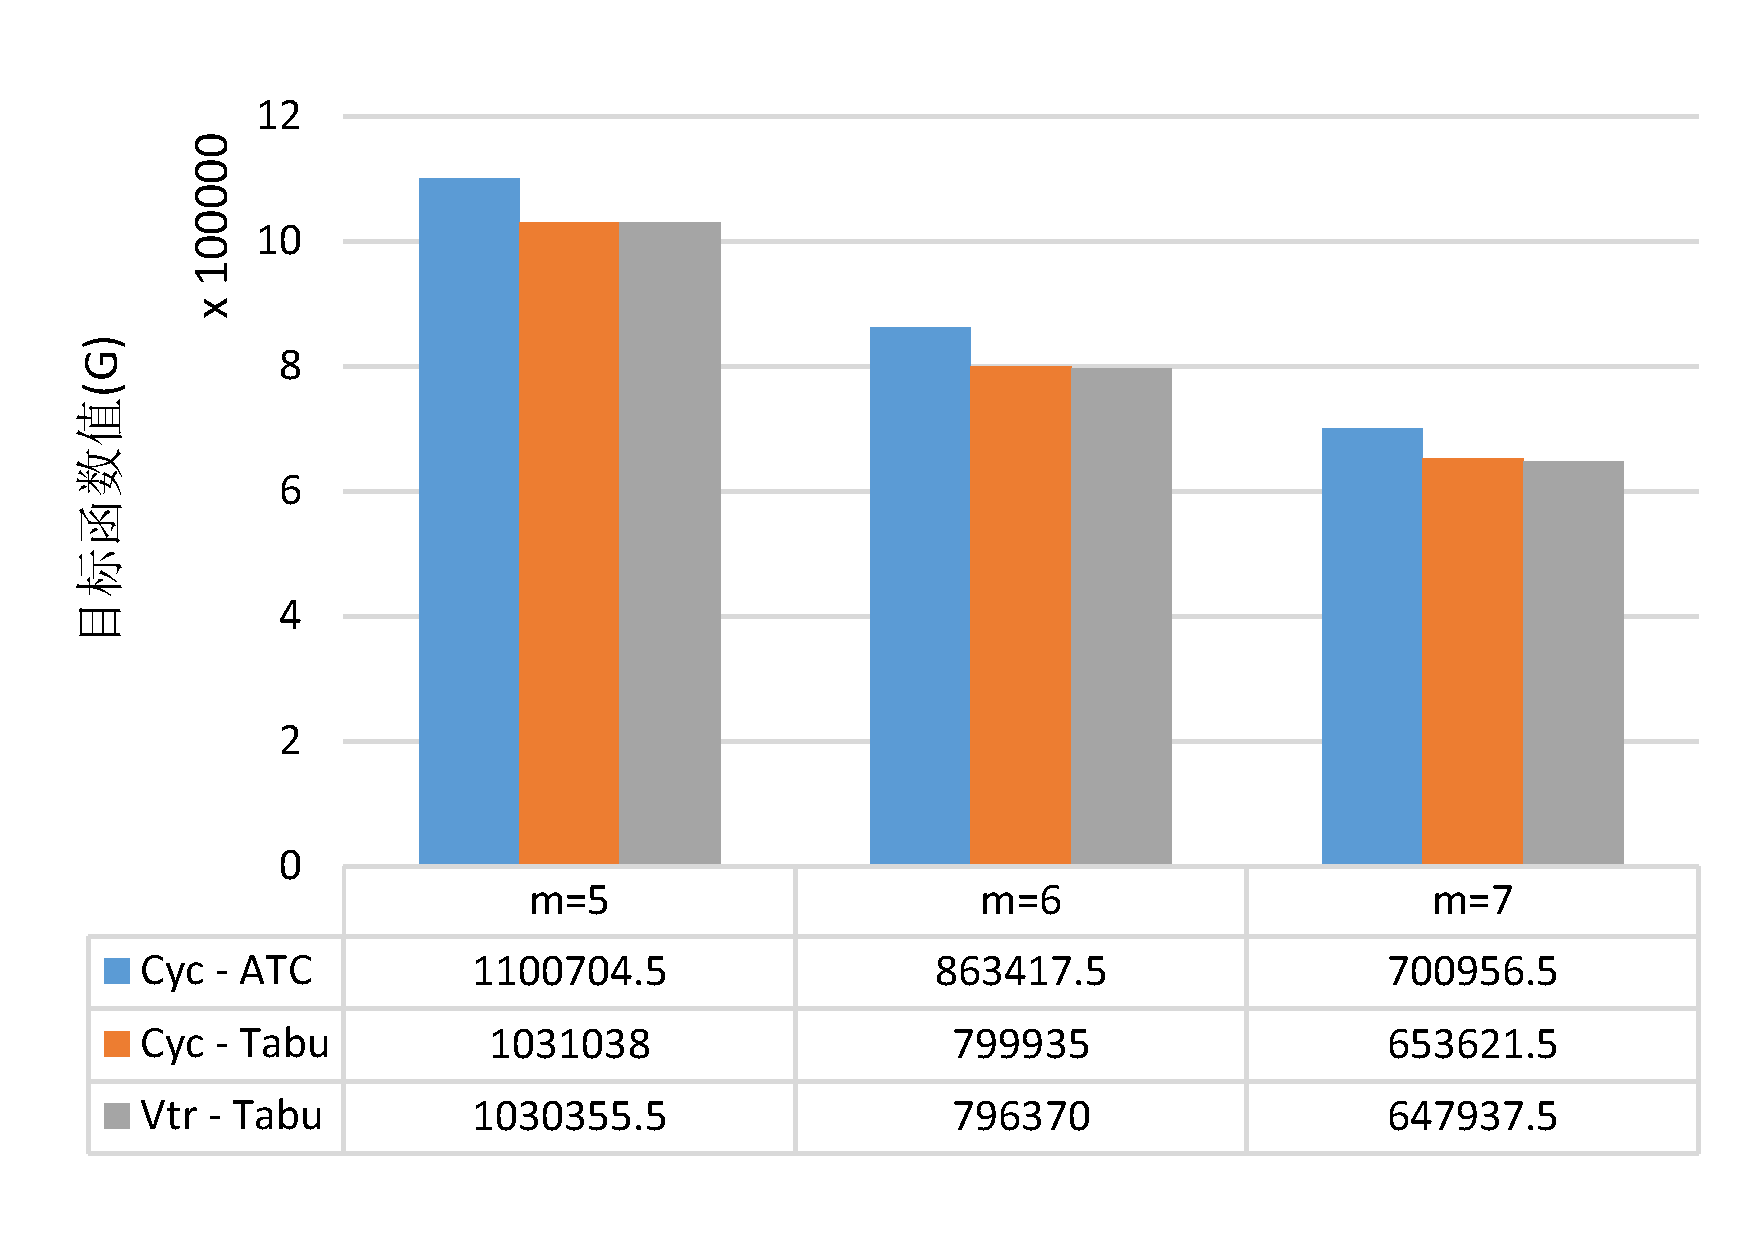
\includegraphics[height = 6cm, angle = -90]{basic_05_300}}\\
\subfloat[$n = 500$]{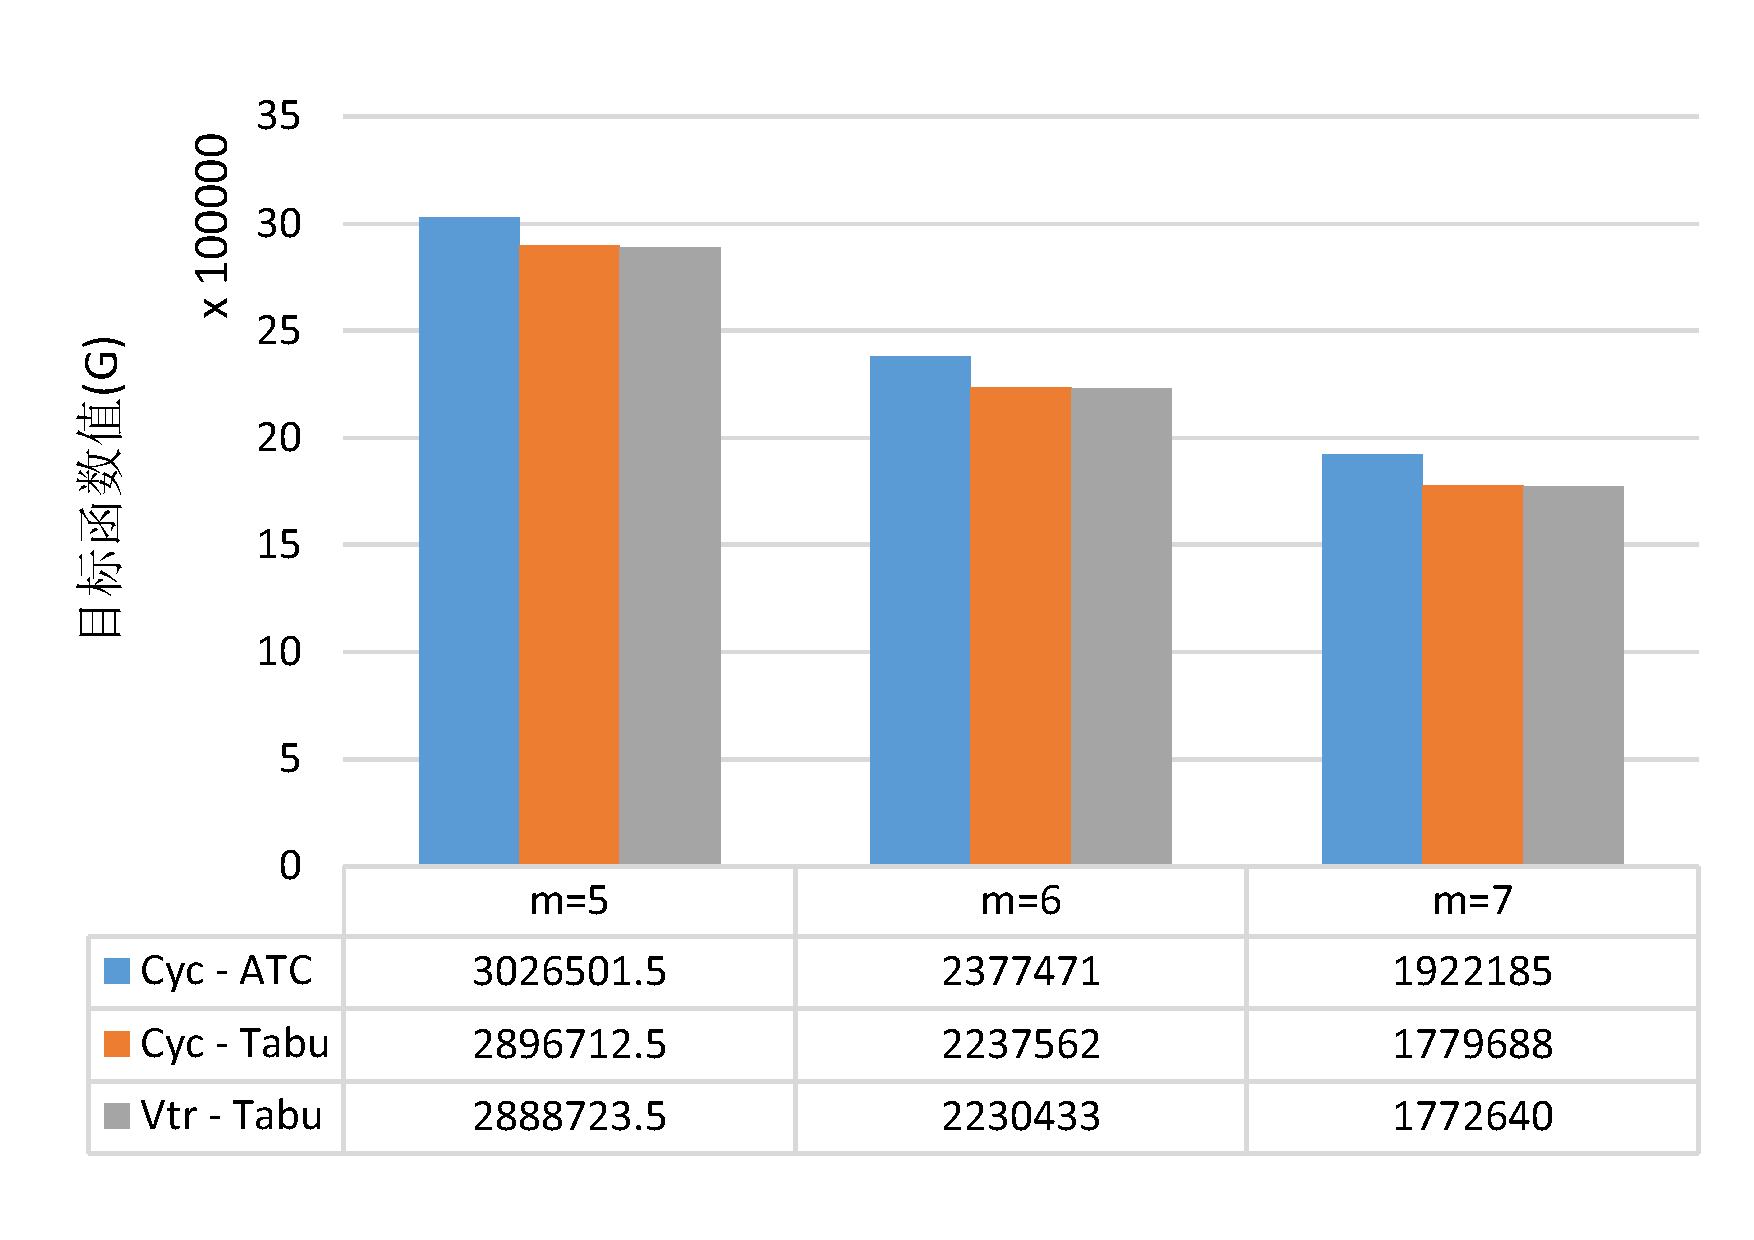
\includegraphics[height = 6cm, angle = -90]{basic_05_500}}
\subfloat[$n = 750$]{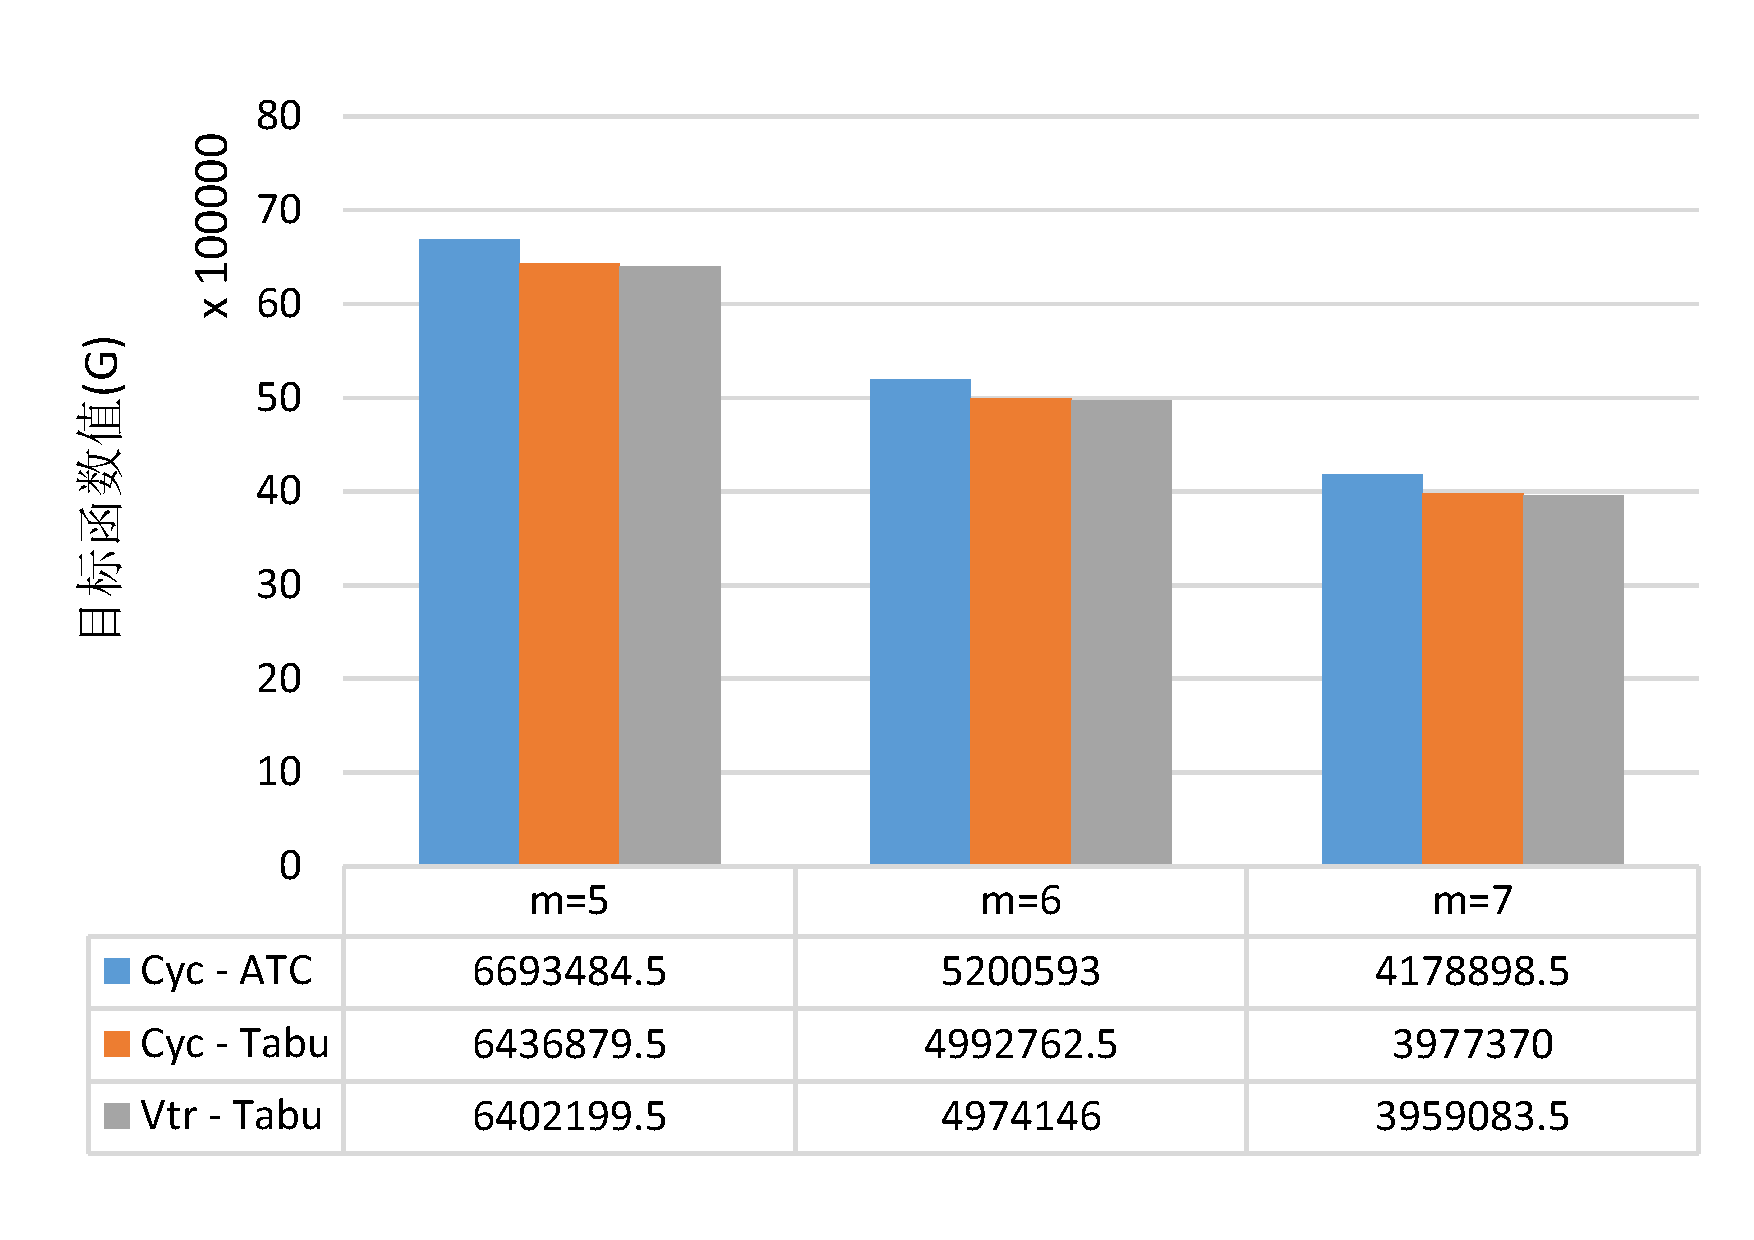
\includegraphics[height = 6cm, angle = -90]{basic_05_750}}
\subfloat[$n = 1000$]{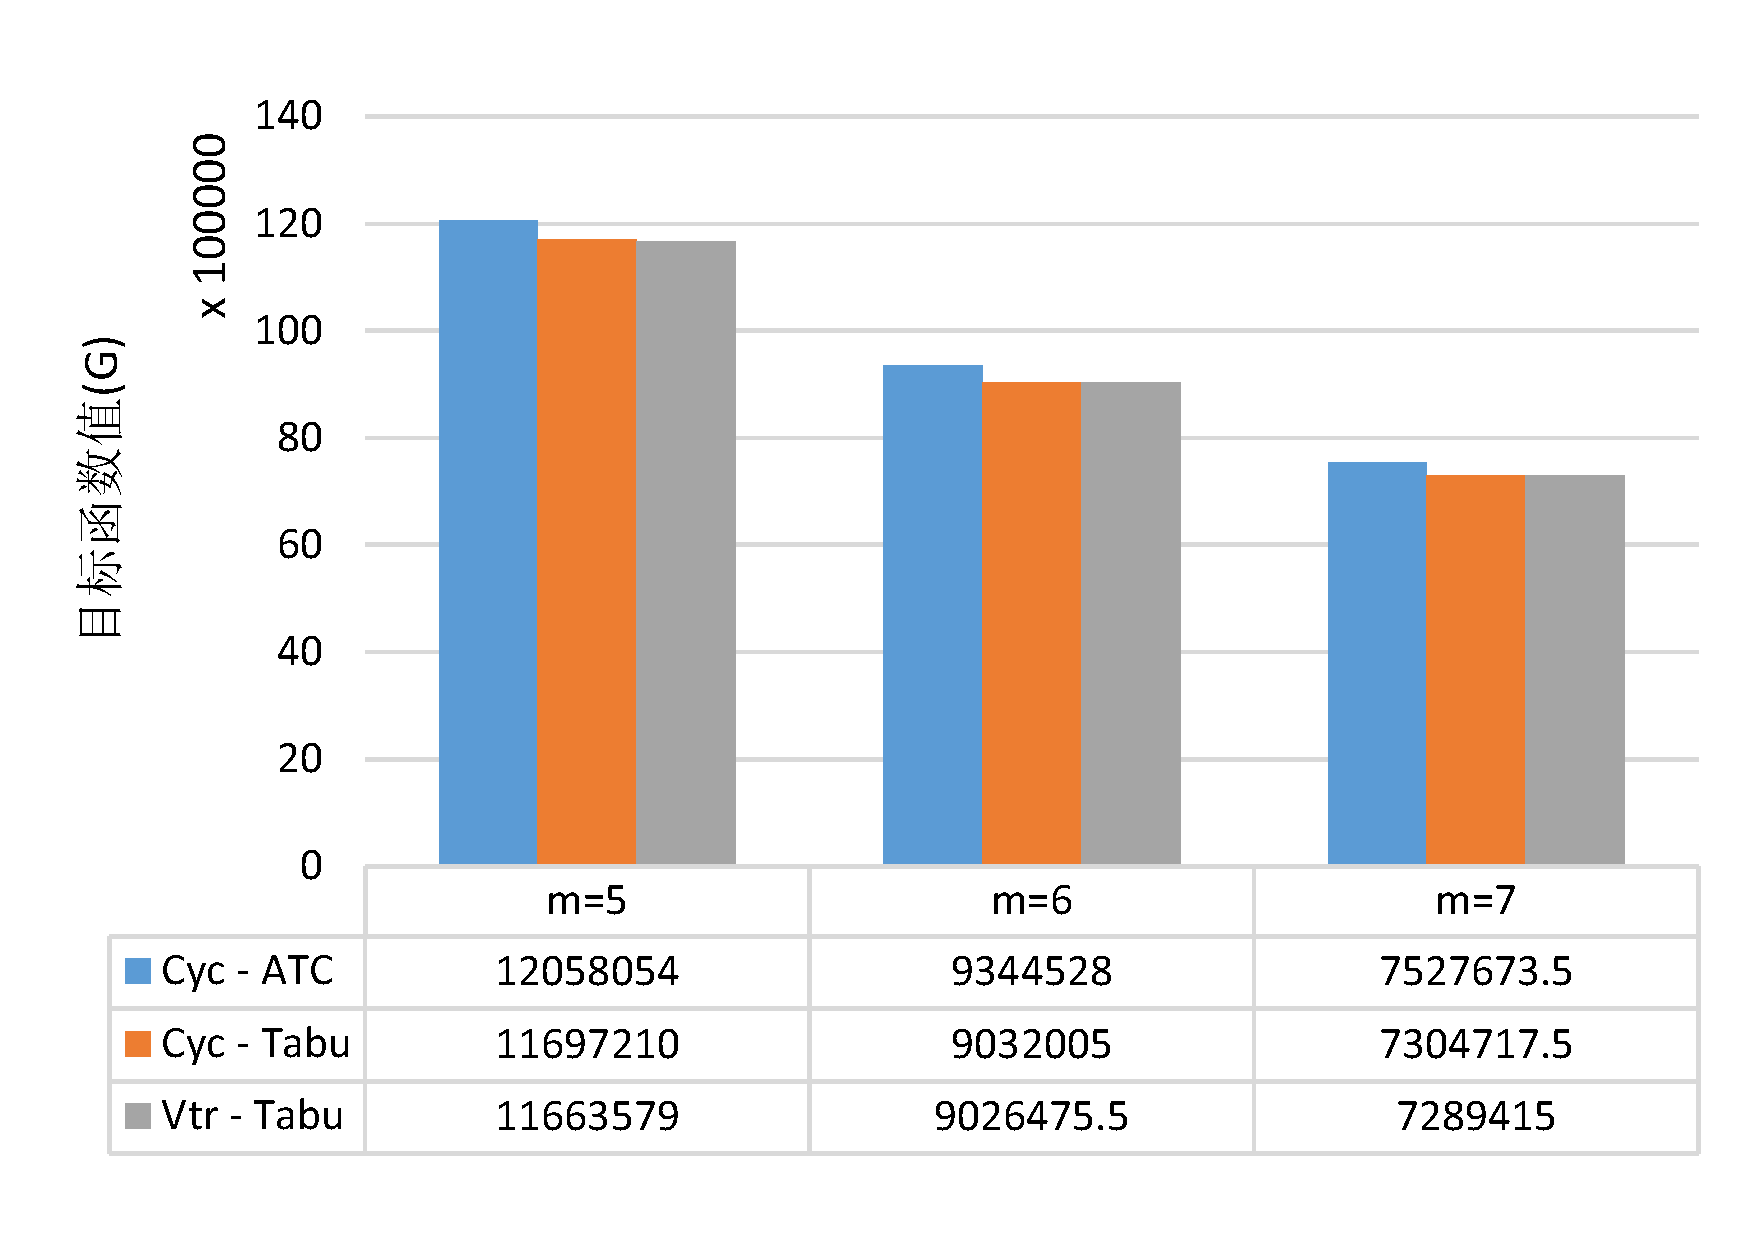
\includegraphics[height = 6cm, angle = -90]{basic_05_1000}}
\caption{\label{fig:result2}模型$1$的Cyc -- ATC、Cyc -- Tabu、Vtr -- Tabu 算法求解目标函数值比较$(\lambda_1 = 0.5)$}
\end{sidewaysfigure}

\begin{sidewaysfigure}
\centering
\subfloat[$n = 20$]{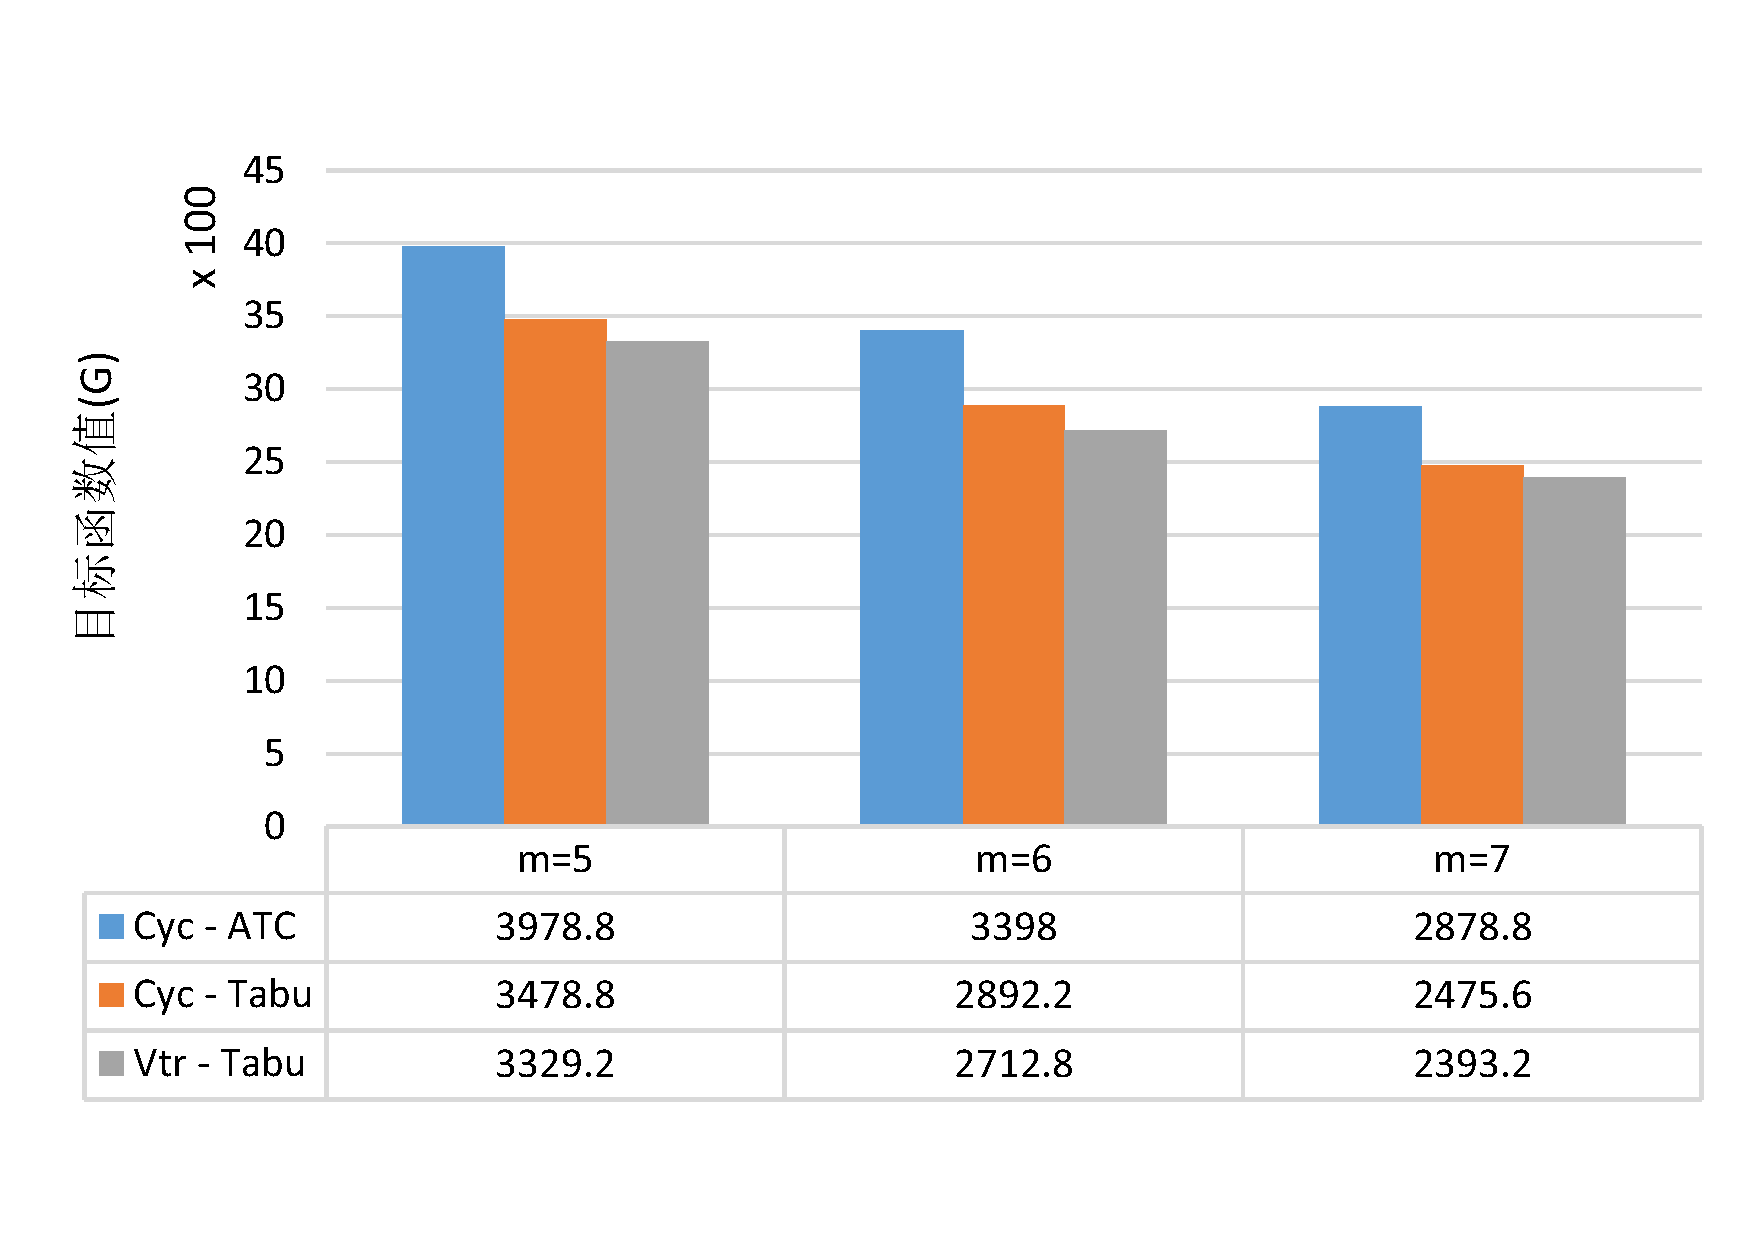
\includegraphics[height = 6cm, angle = -90]{basic_06_20}}
\subfloat[$n = 30$]{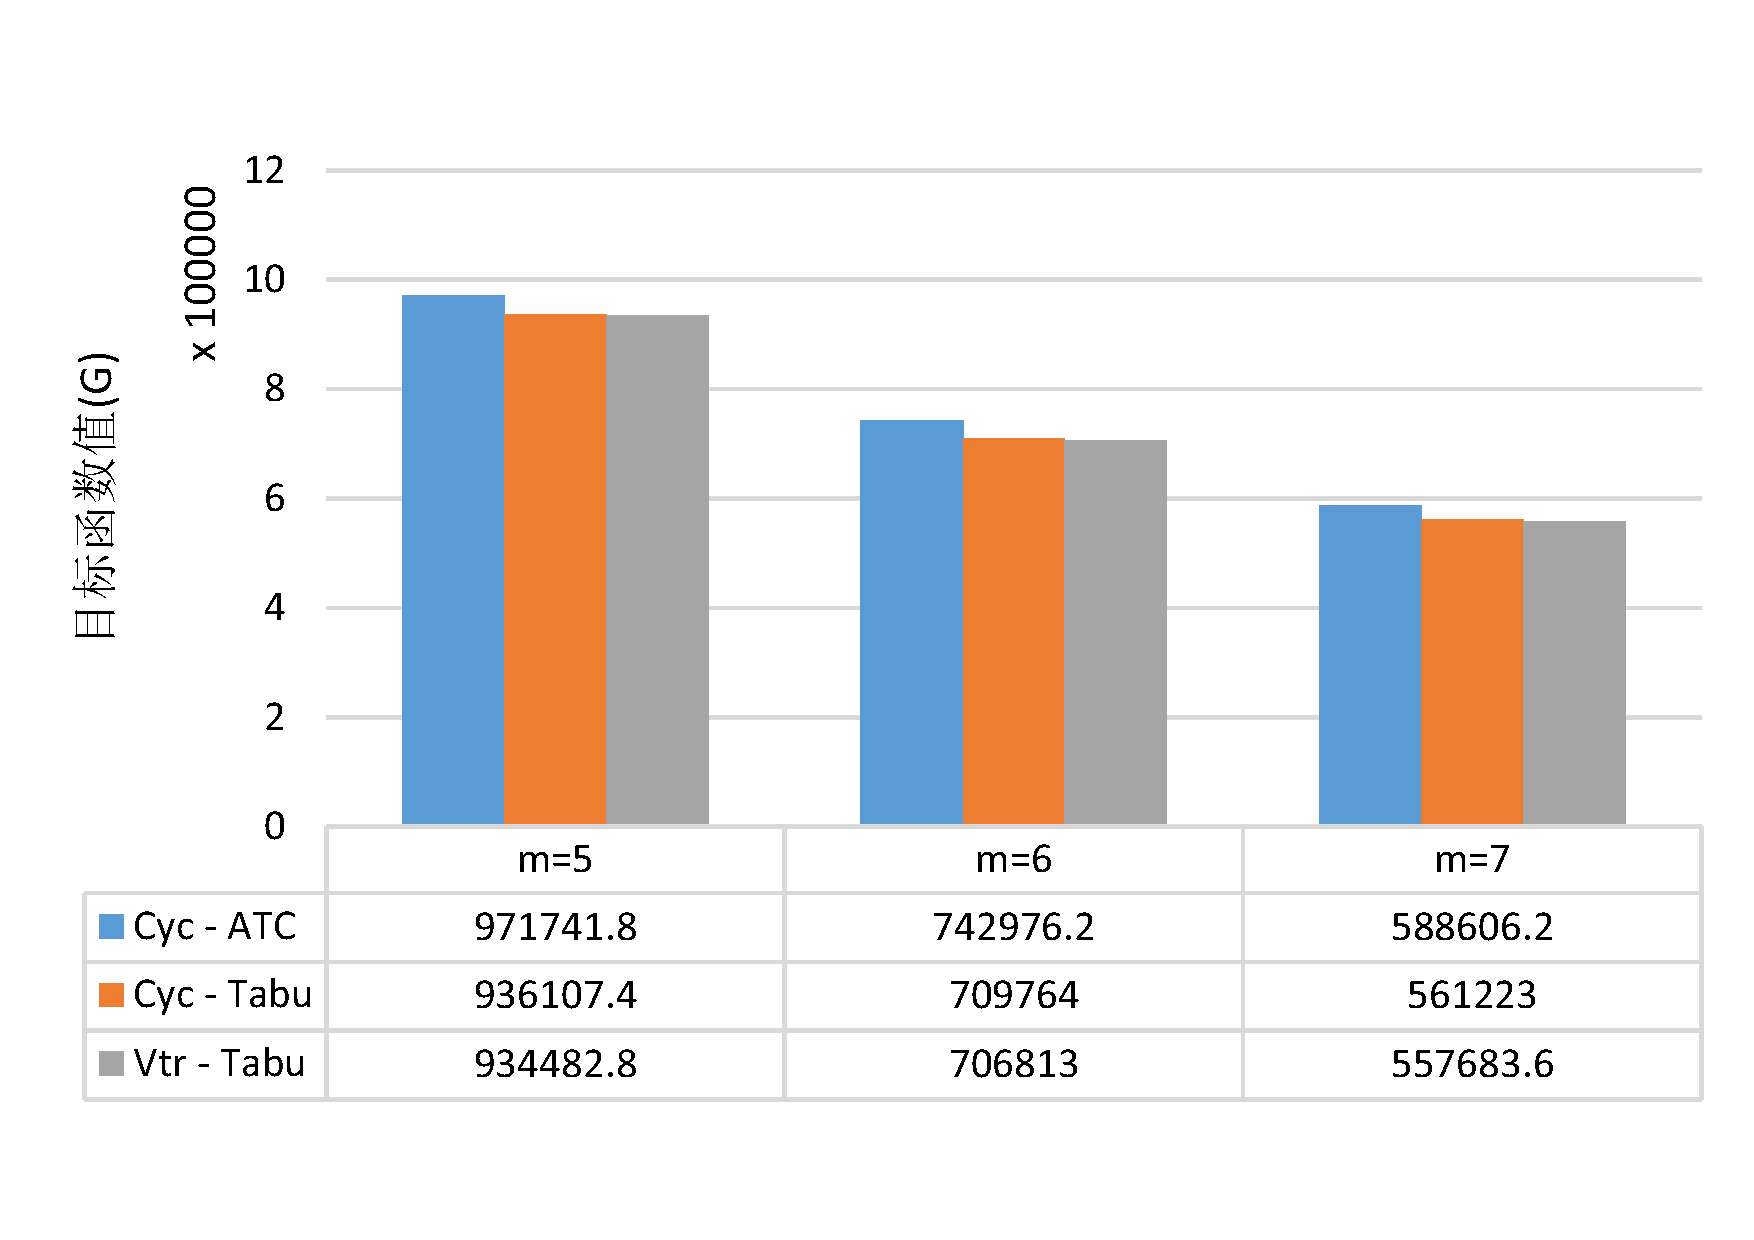
\includegraphics[height = 6cm, angle = -90]{basic_06_300}}
\subfloat[$n = 50$]{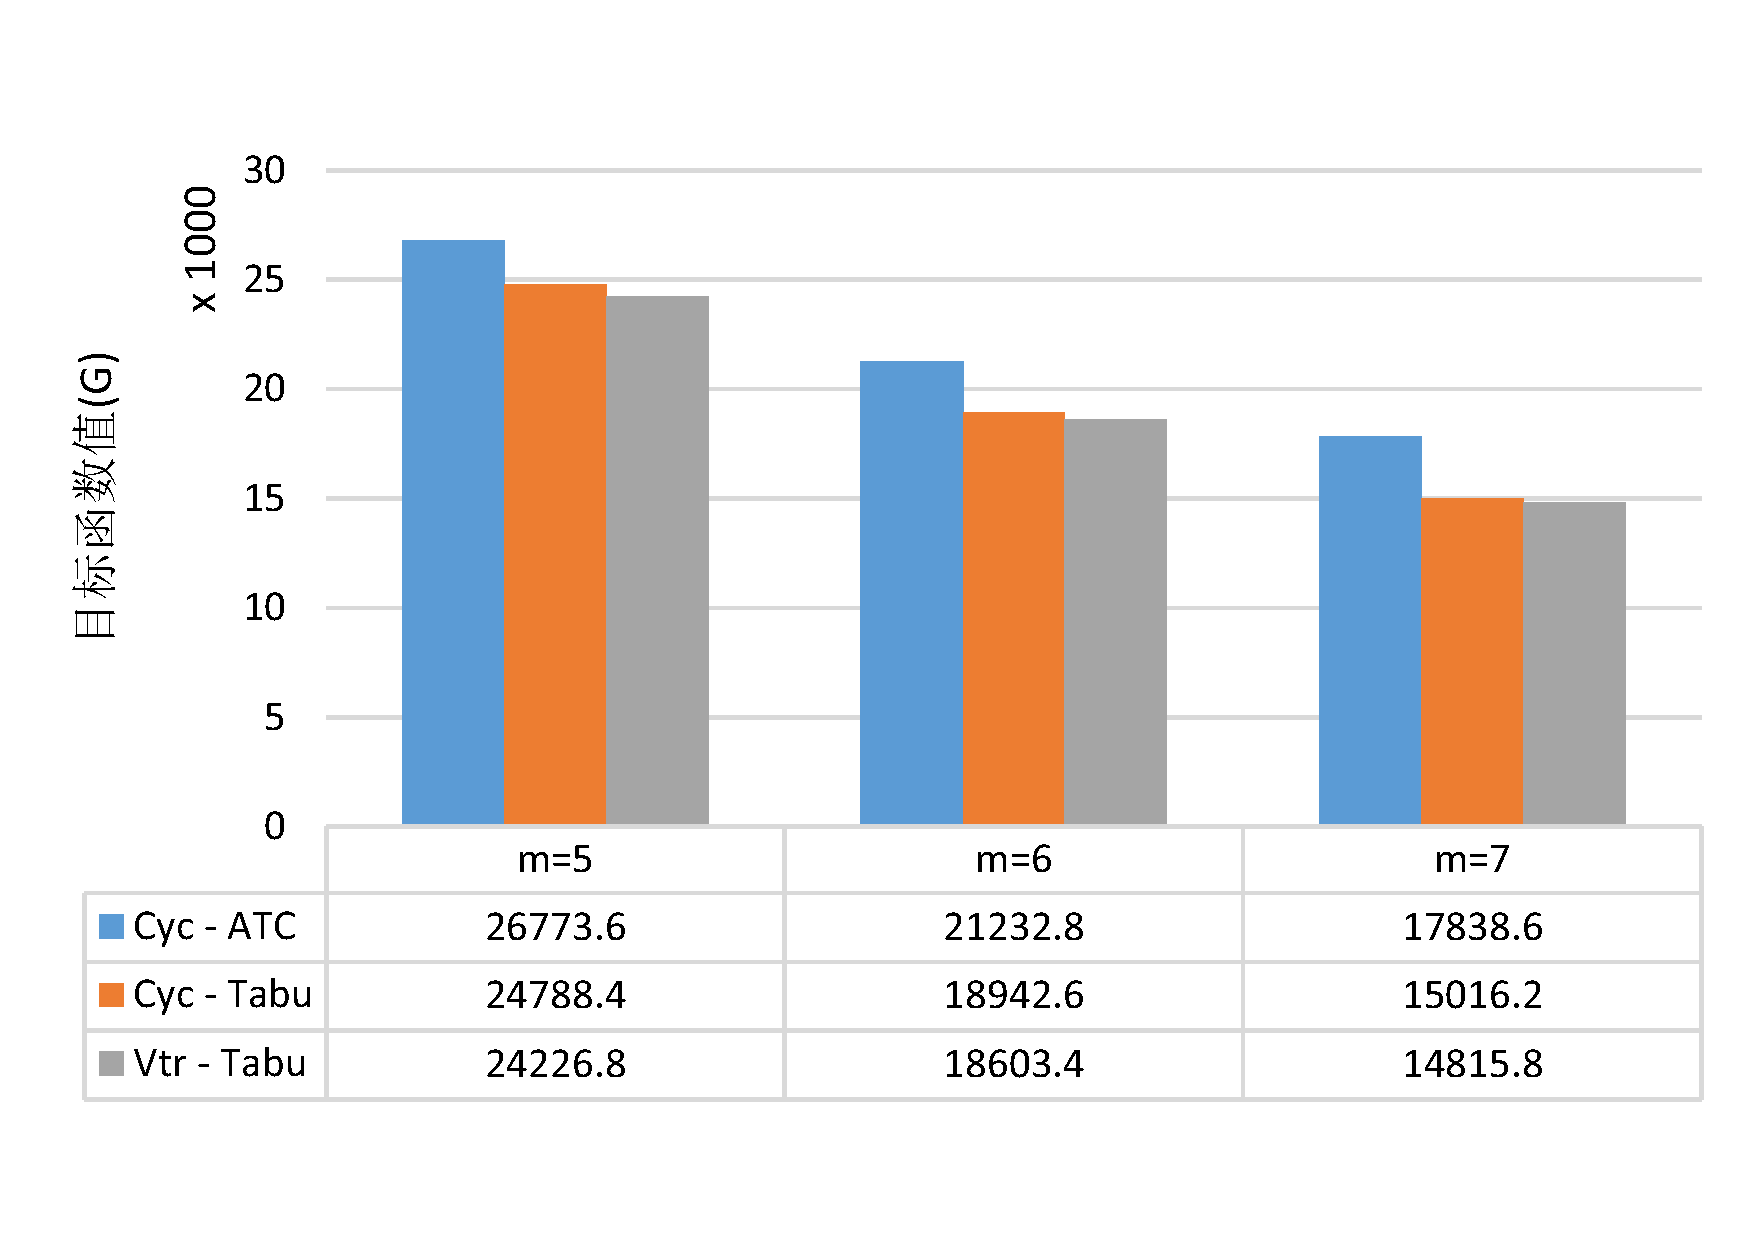
\includegraphics[height = 6cm, angle = -90]{basic_06_50}}
\subfloat[$n = 70$]{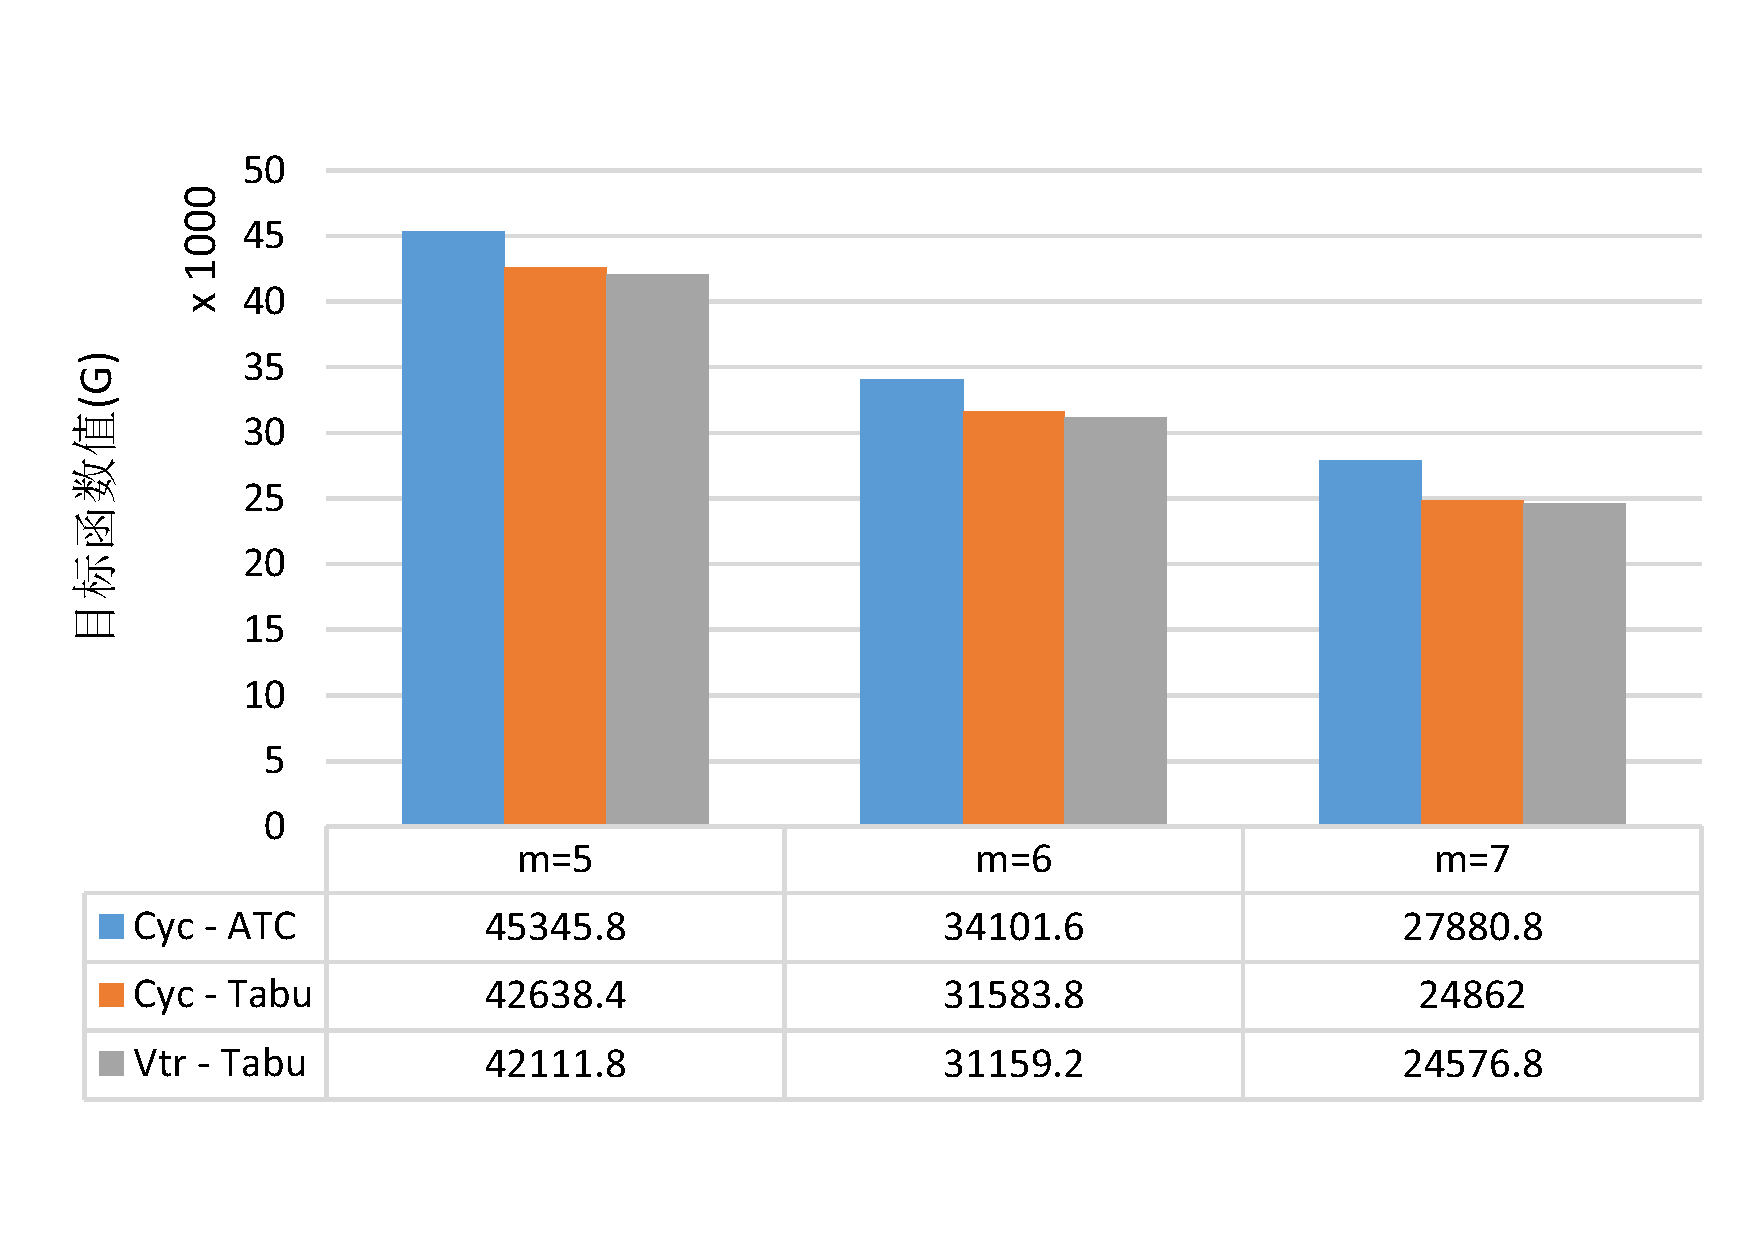
\includegraphics[height = 6cm, angle = -90]{basic_06_70}}\\
\subfloat[$n = 100$]{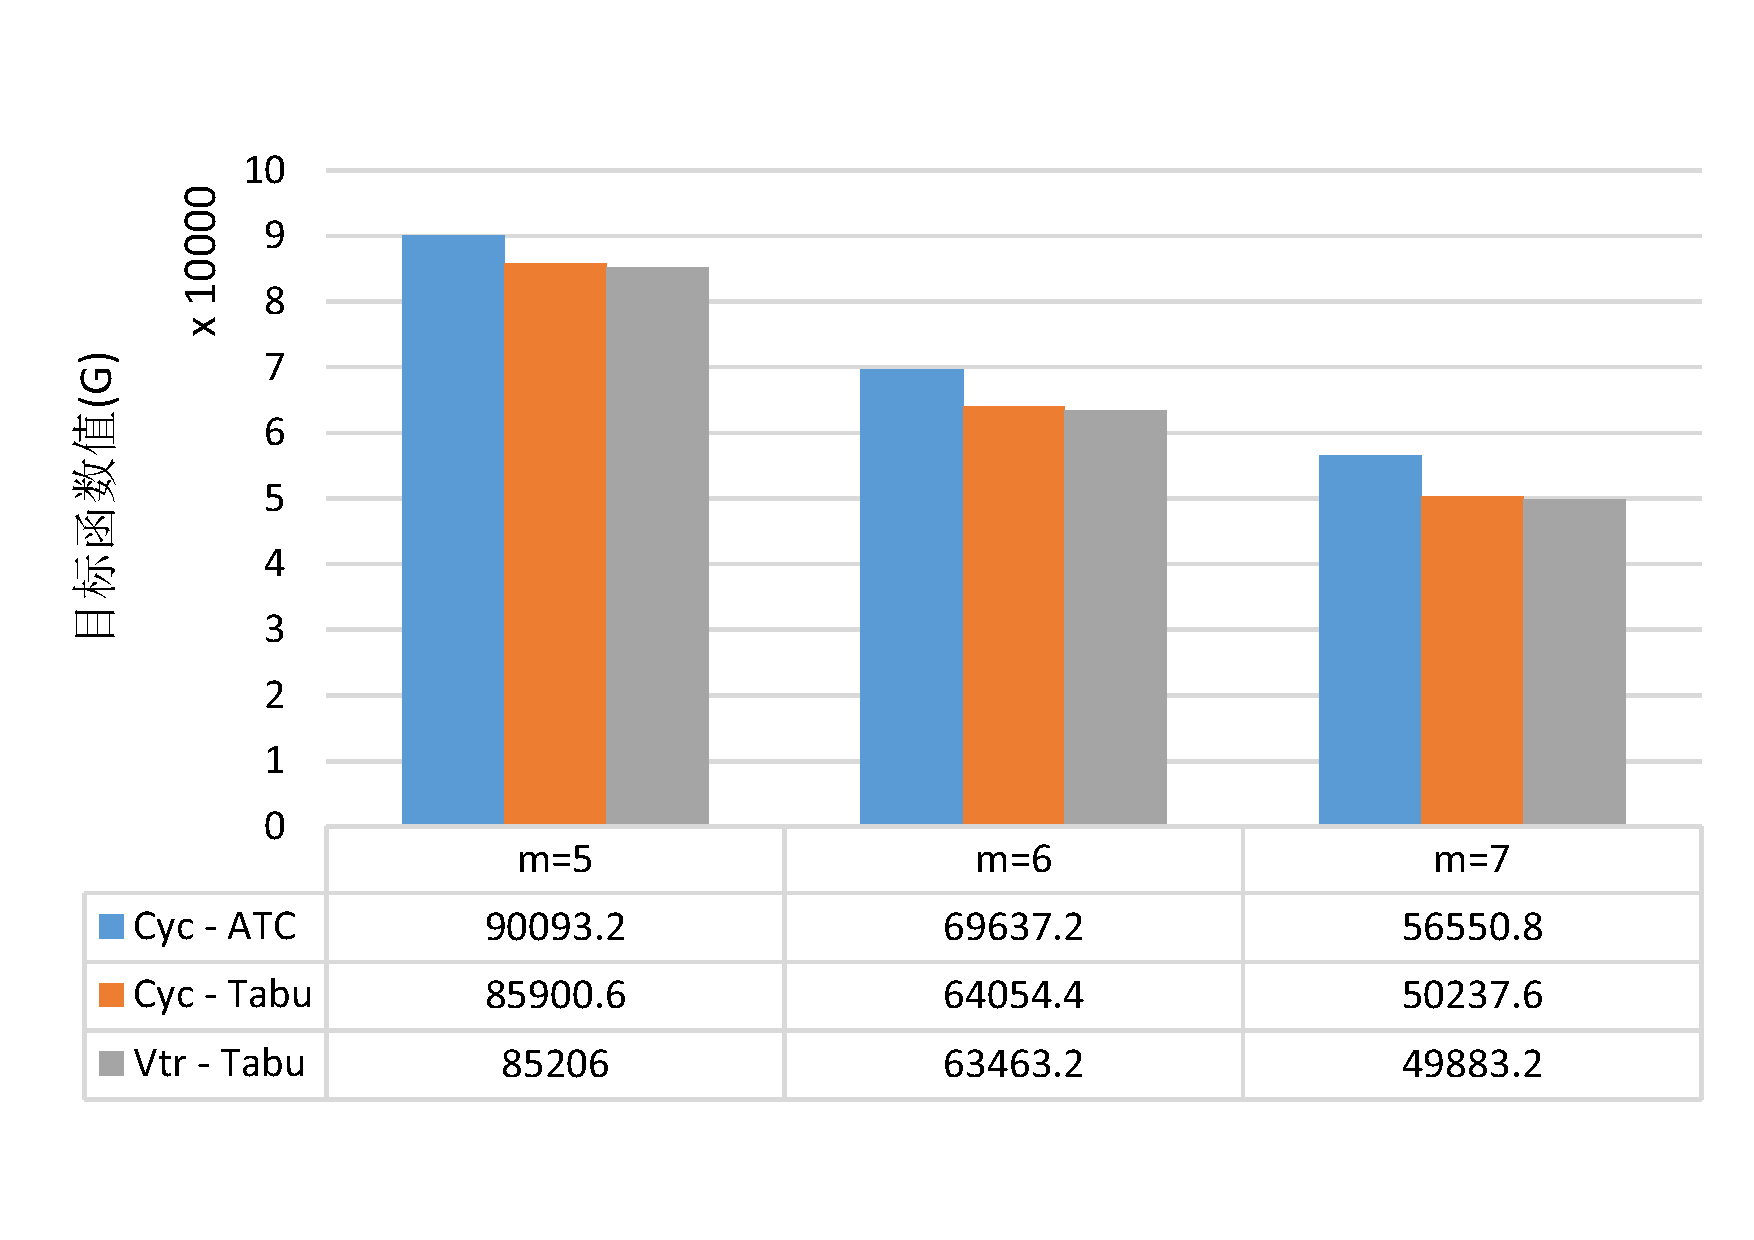
\includegraphics[height = 6cm, angle = -90]{basic_06_100}}
\subfloat[$n = 150$]{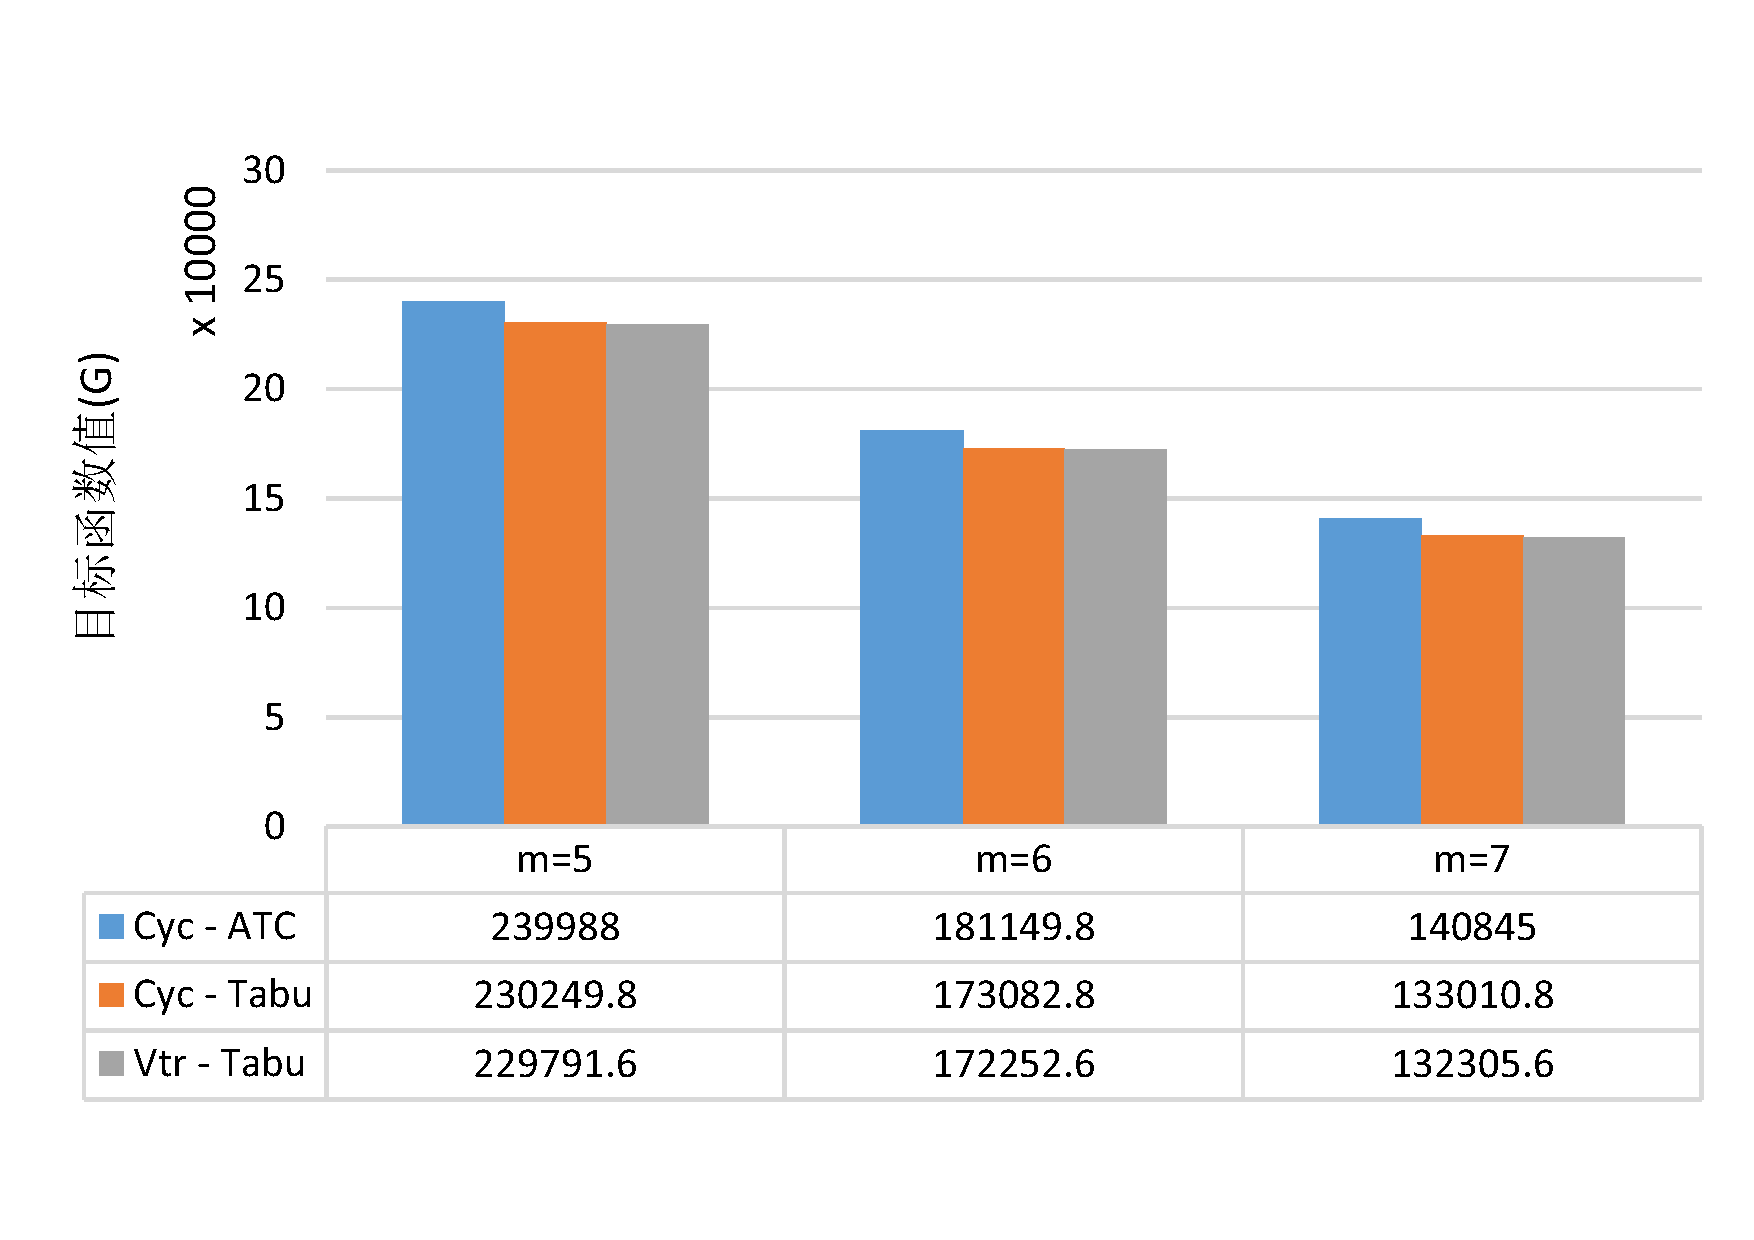
\includegraphics[height = 6cm, angle = -90]{basic_06_150}}
\subfloat[$n = 200$]{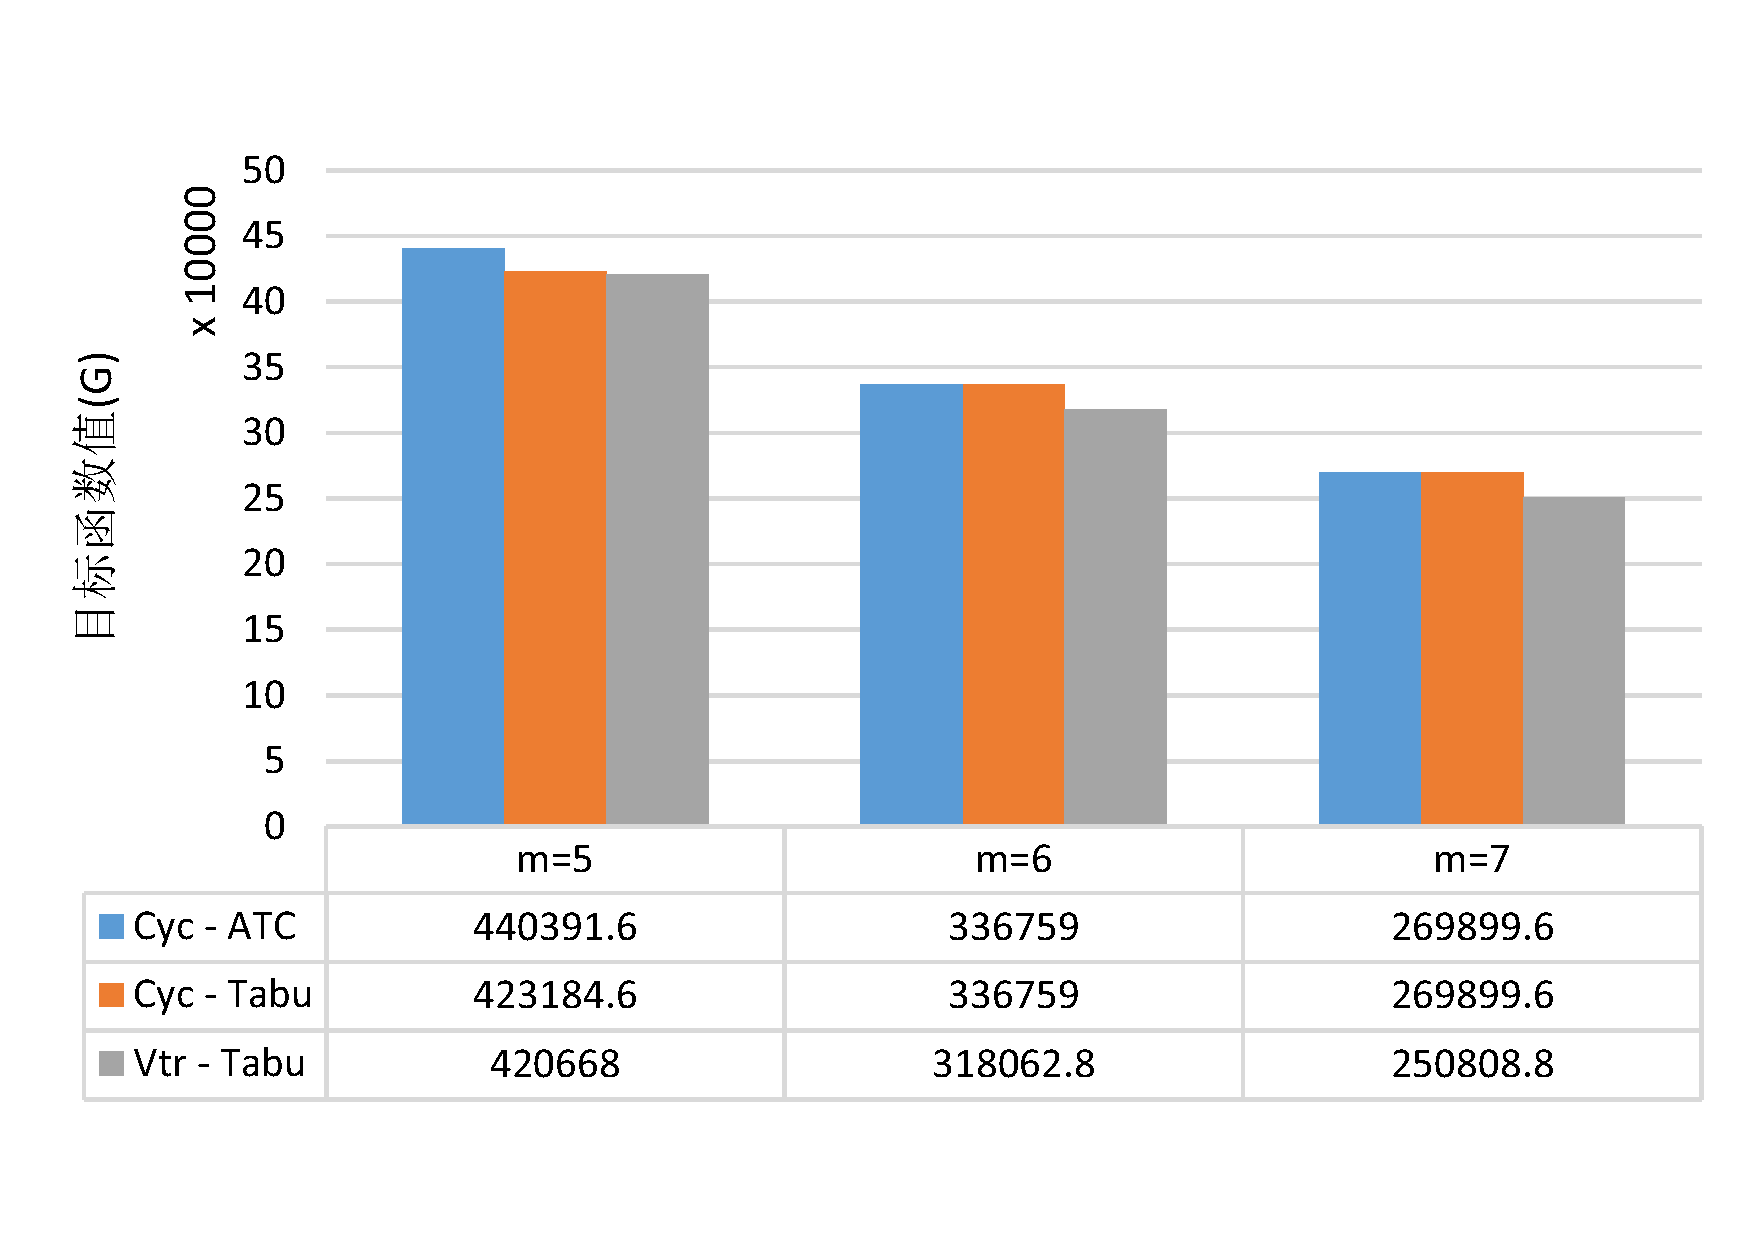
\includegraphics[height = 6cm, angle = -90]{basic_06_200}}
\subfloat[$n = 300$]{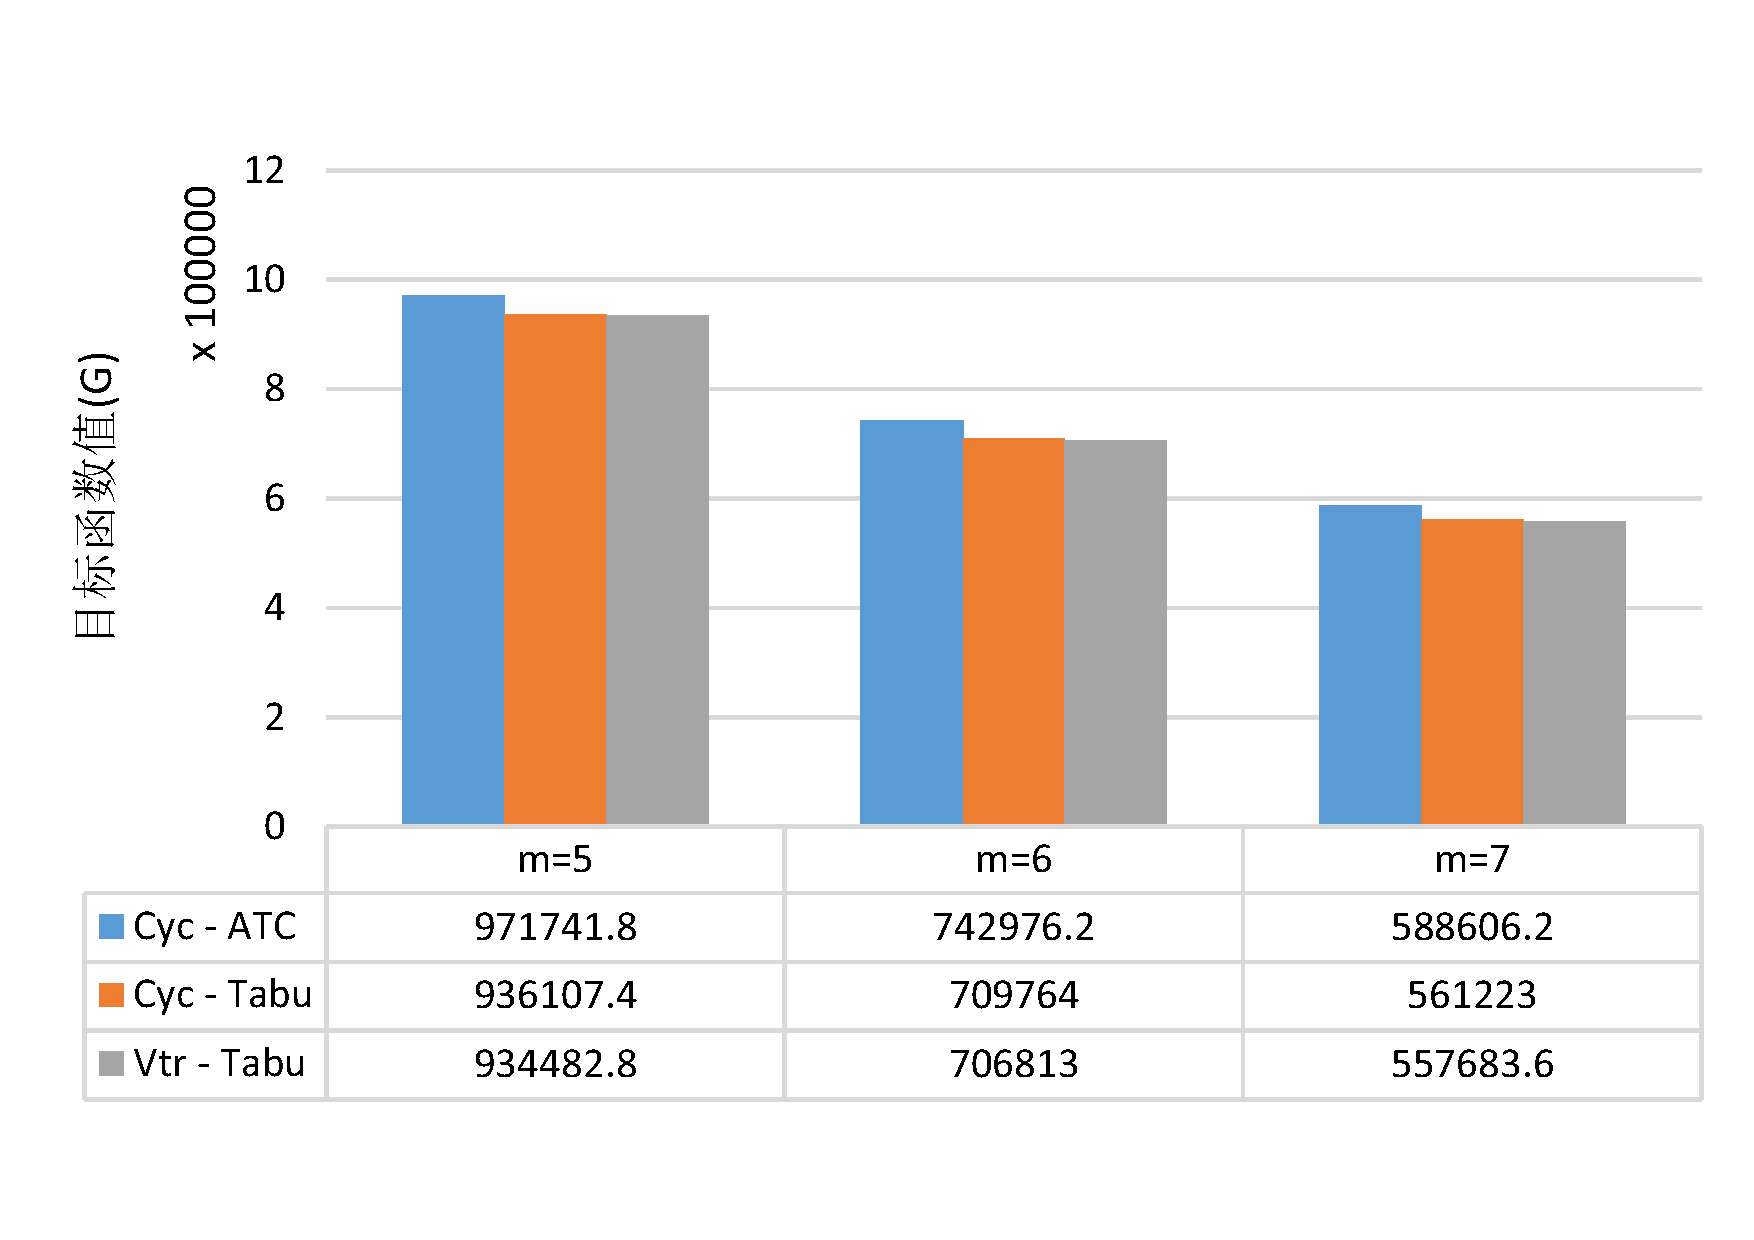
\includegraphics[height = 6cm, angle = -90]{basic_06_300}}\\
\subfloat[$n = 500$]{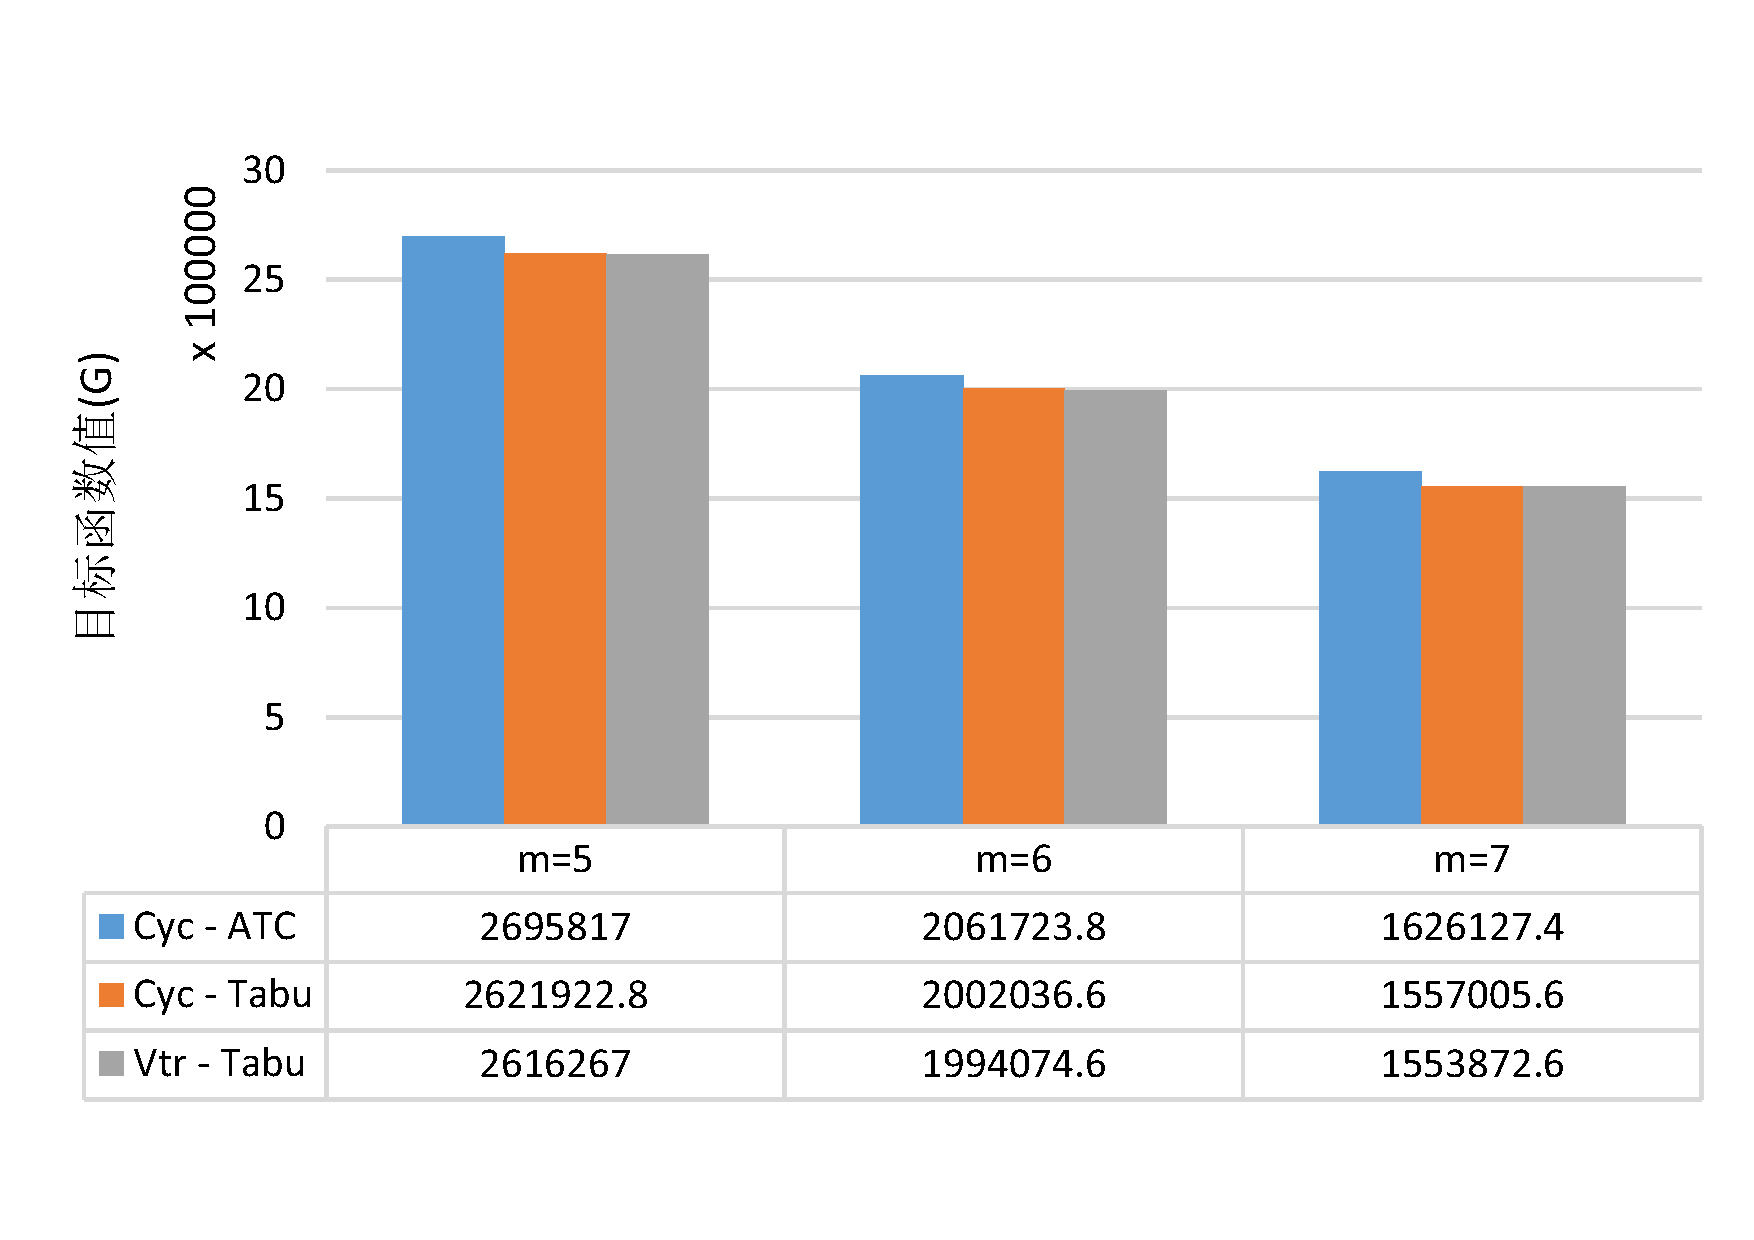
\includegraphics[height = 6cm, angle = -90]{basic_06_500}}
\subfloat[$n = 750$]{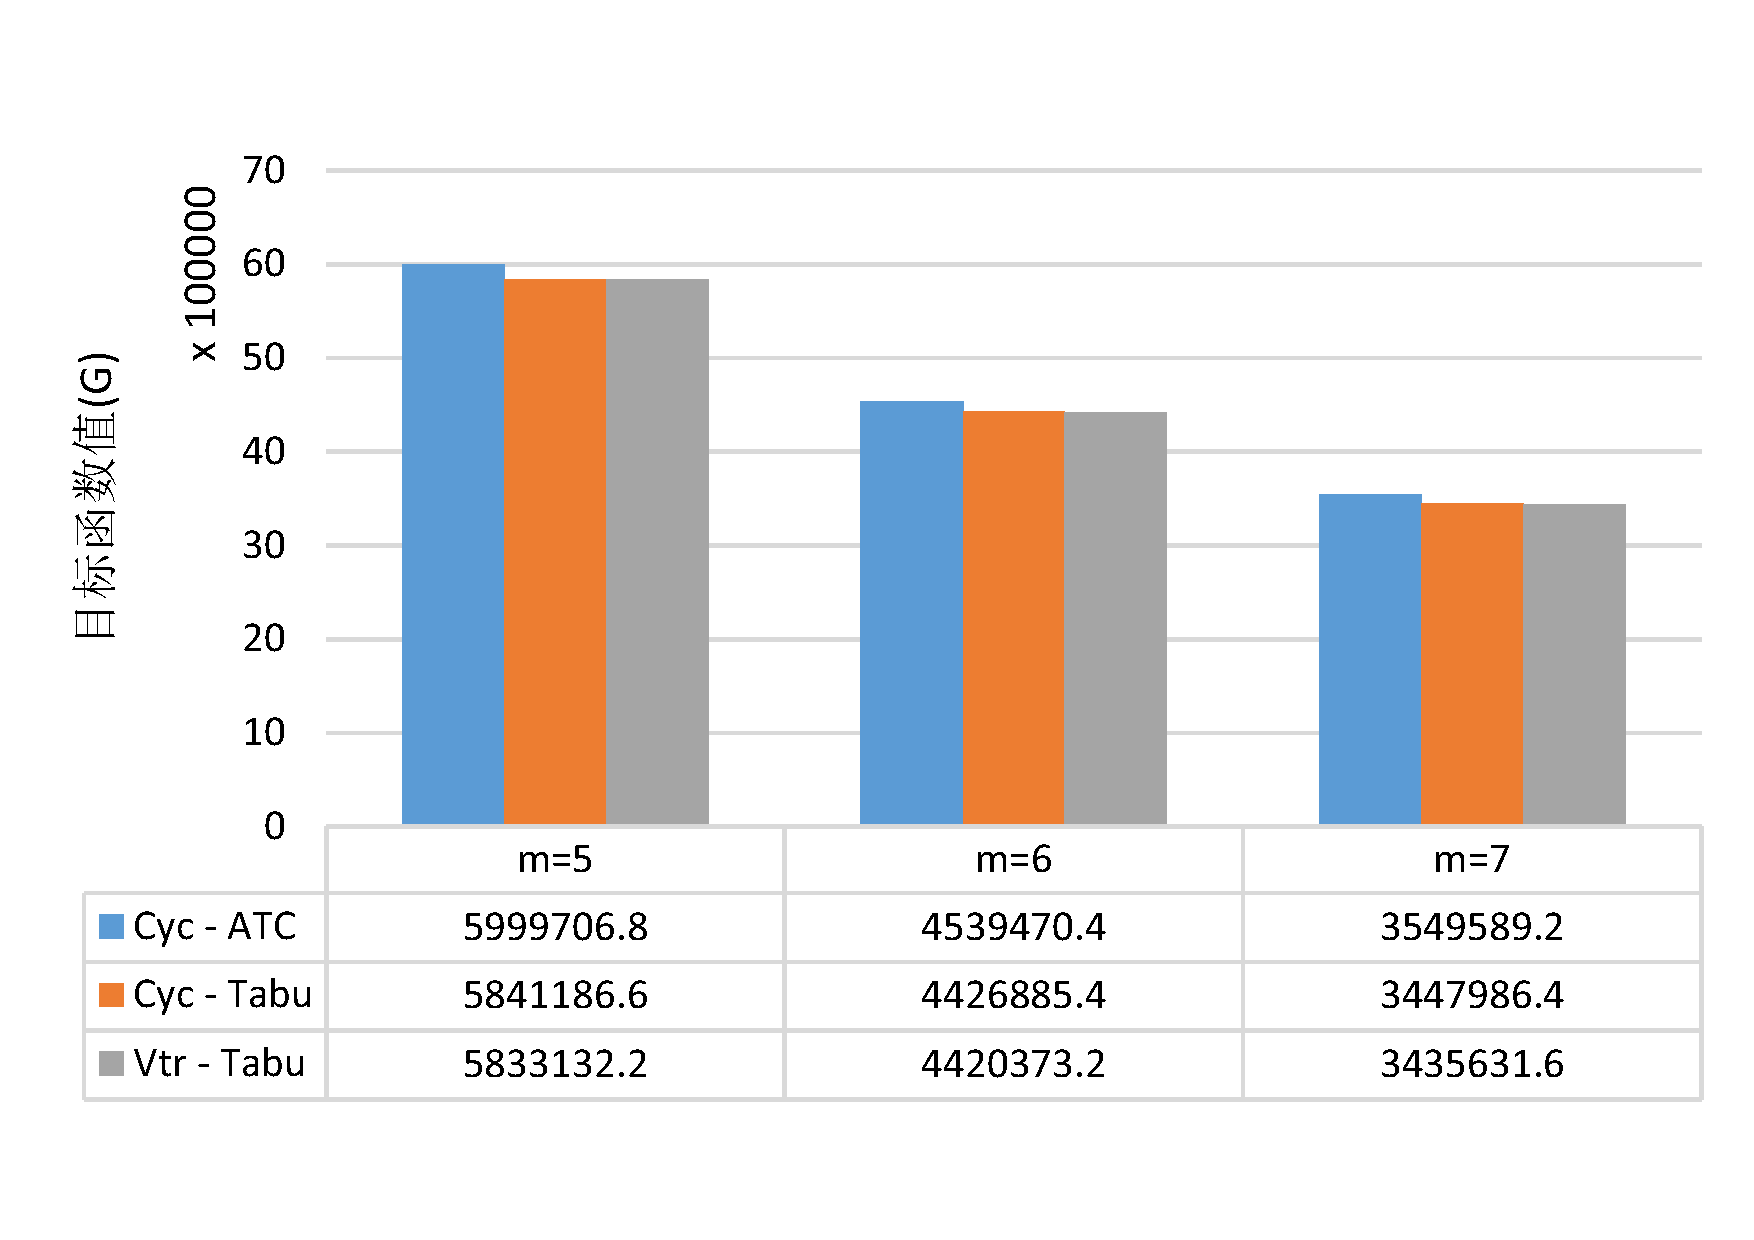
\includegraphics[height = 6cm, angle = -90]{basic_06_750}}
\subfloat[$n = 1000$]{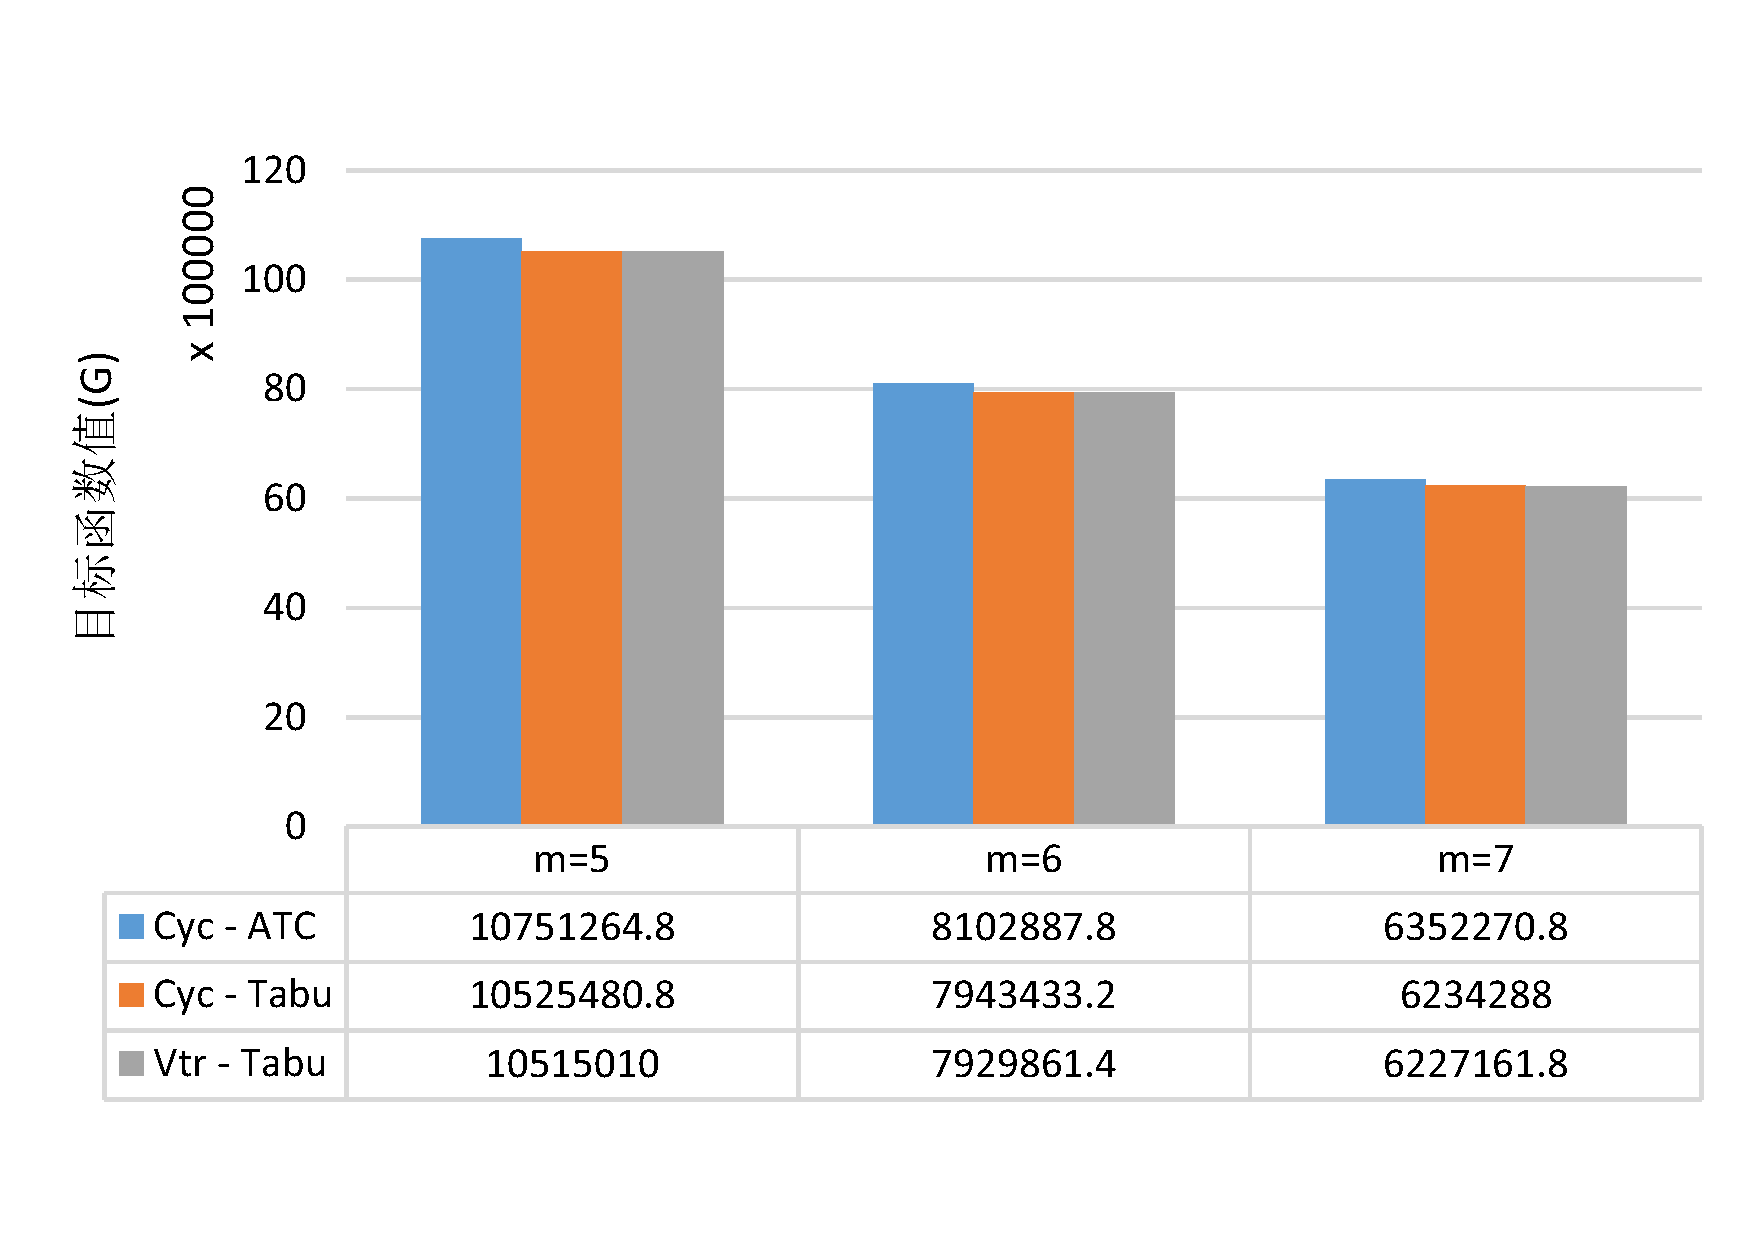
\includegraphics[height = 6cm, angle = -90]{basic_06_1000}}
\caption{\label{fig:result3}模型$1$的Cyc -- ATC、Cyc -- Tabu、Vtr -- Tabu 算法求解目标函数值比较$(\lambda_1 = 0.6)$}
\end{sidewaysfigure}

\begin{sidewaysfigure}
\centering
\subfloat[$n = 20$]{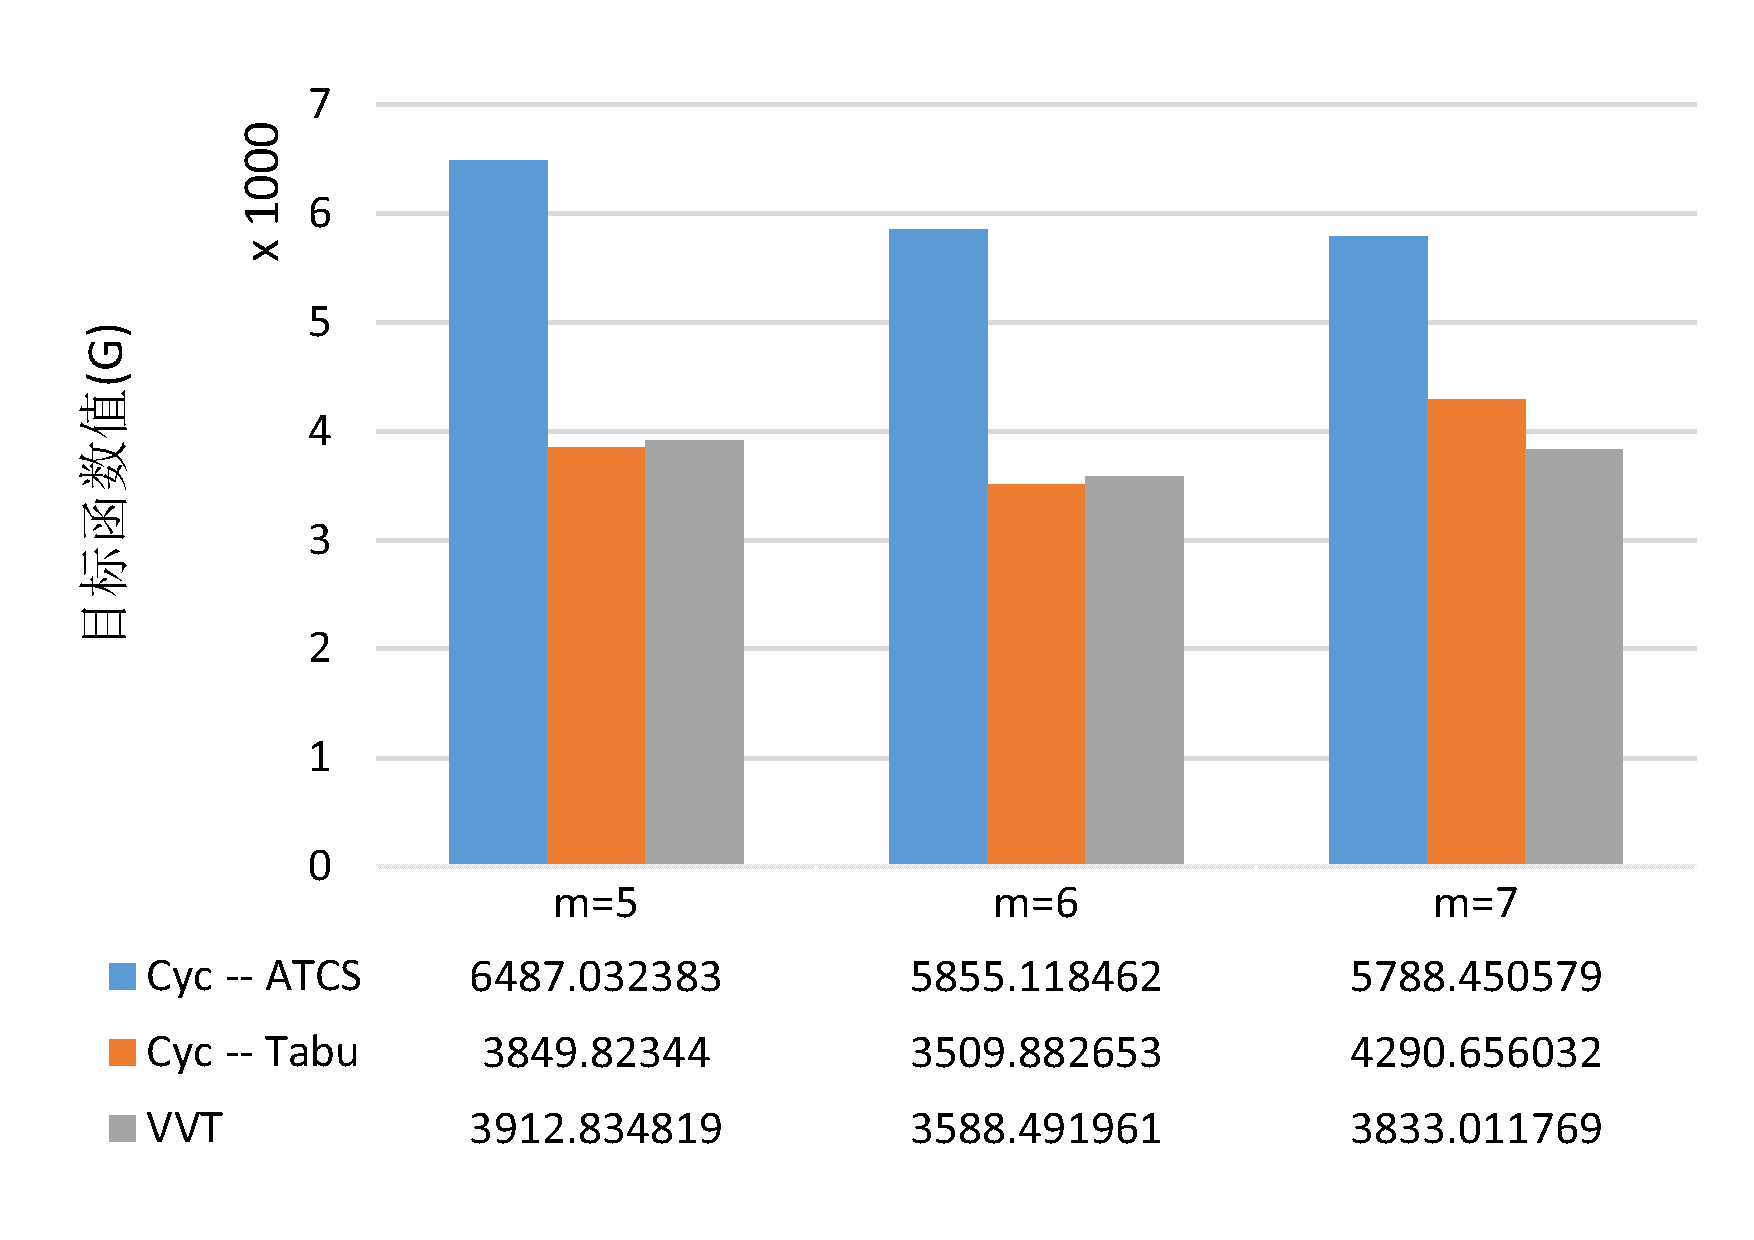
\includegraphics[height = 6cm, angle = -90]{continue_04_20}}
\subfloat[$n = 30$]{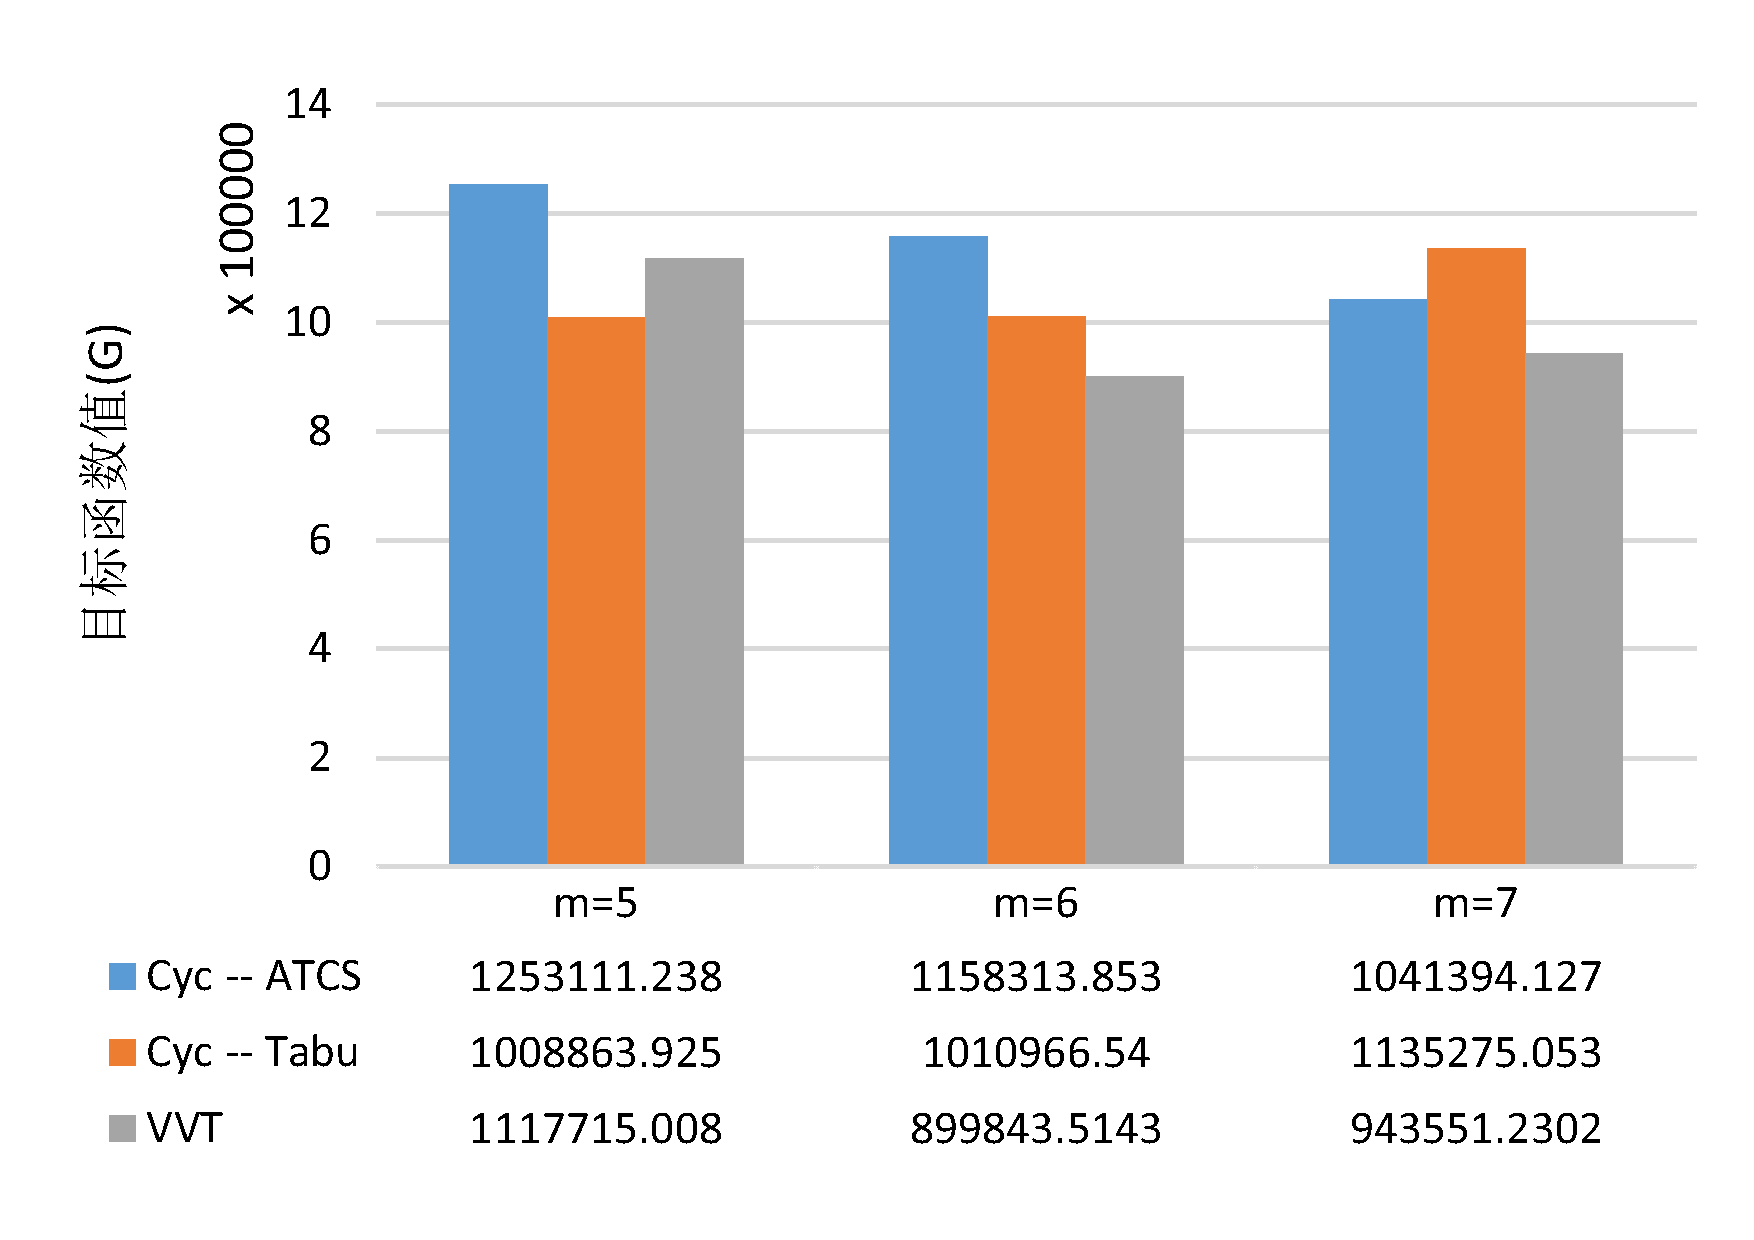
\includegraphics[height = 6cm, angle = -90]{continue_04_300}}
\subfloat[$n = 50$]{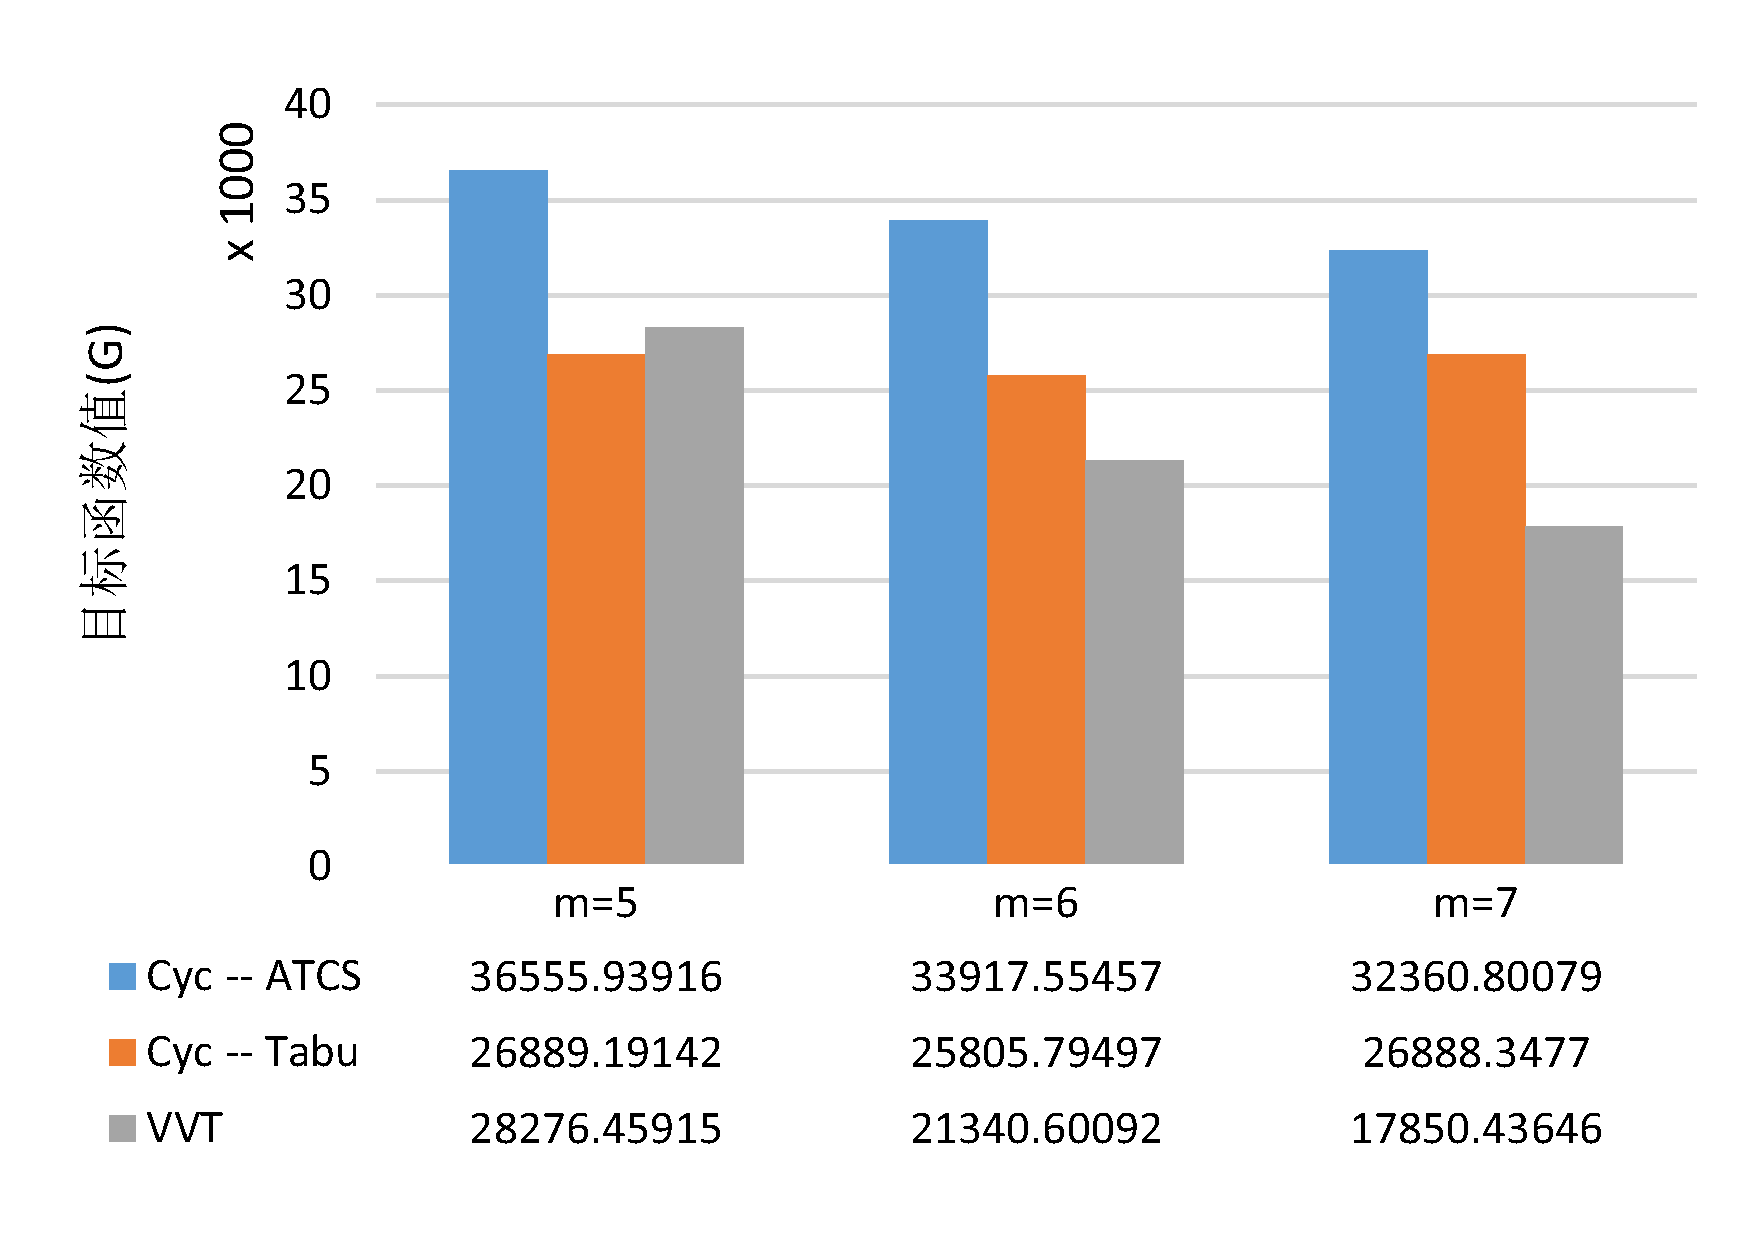
\includegraphics[height = 6cm, angle = -90]{continue_04_50}}
\subfloat[$n = 70$]{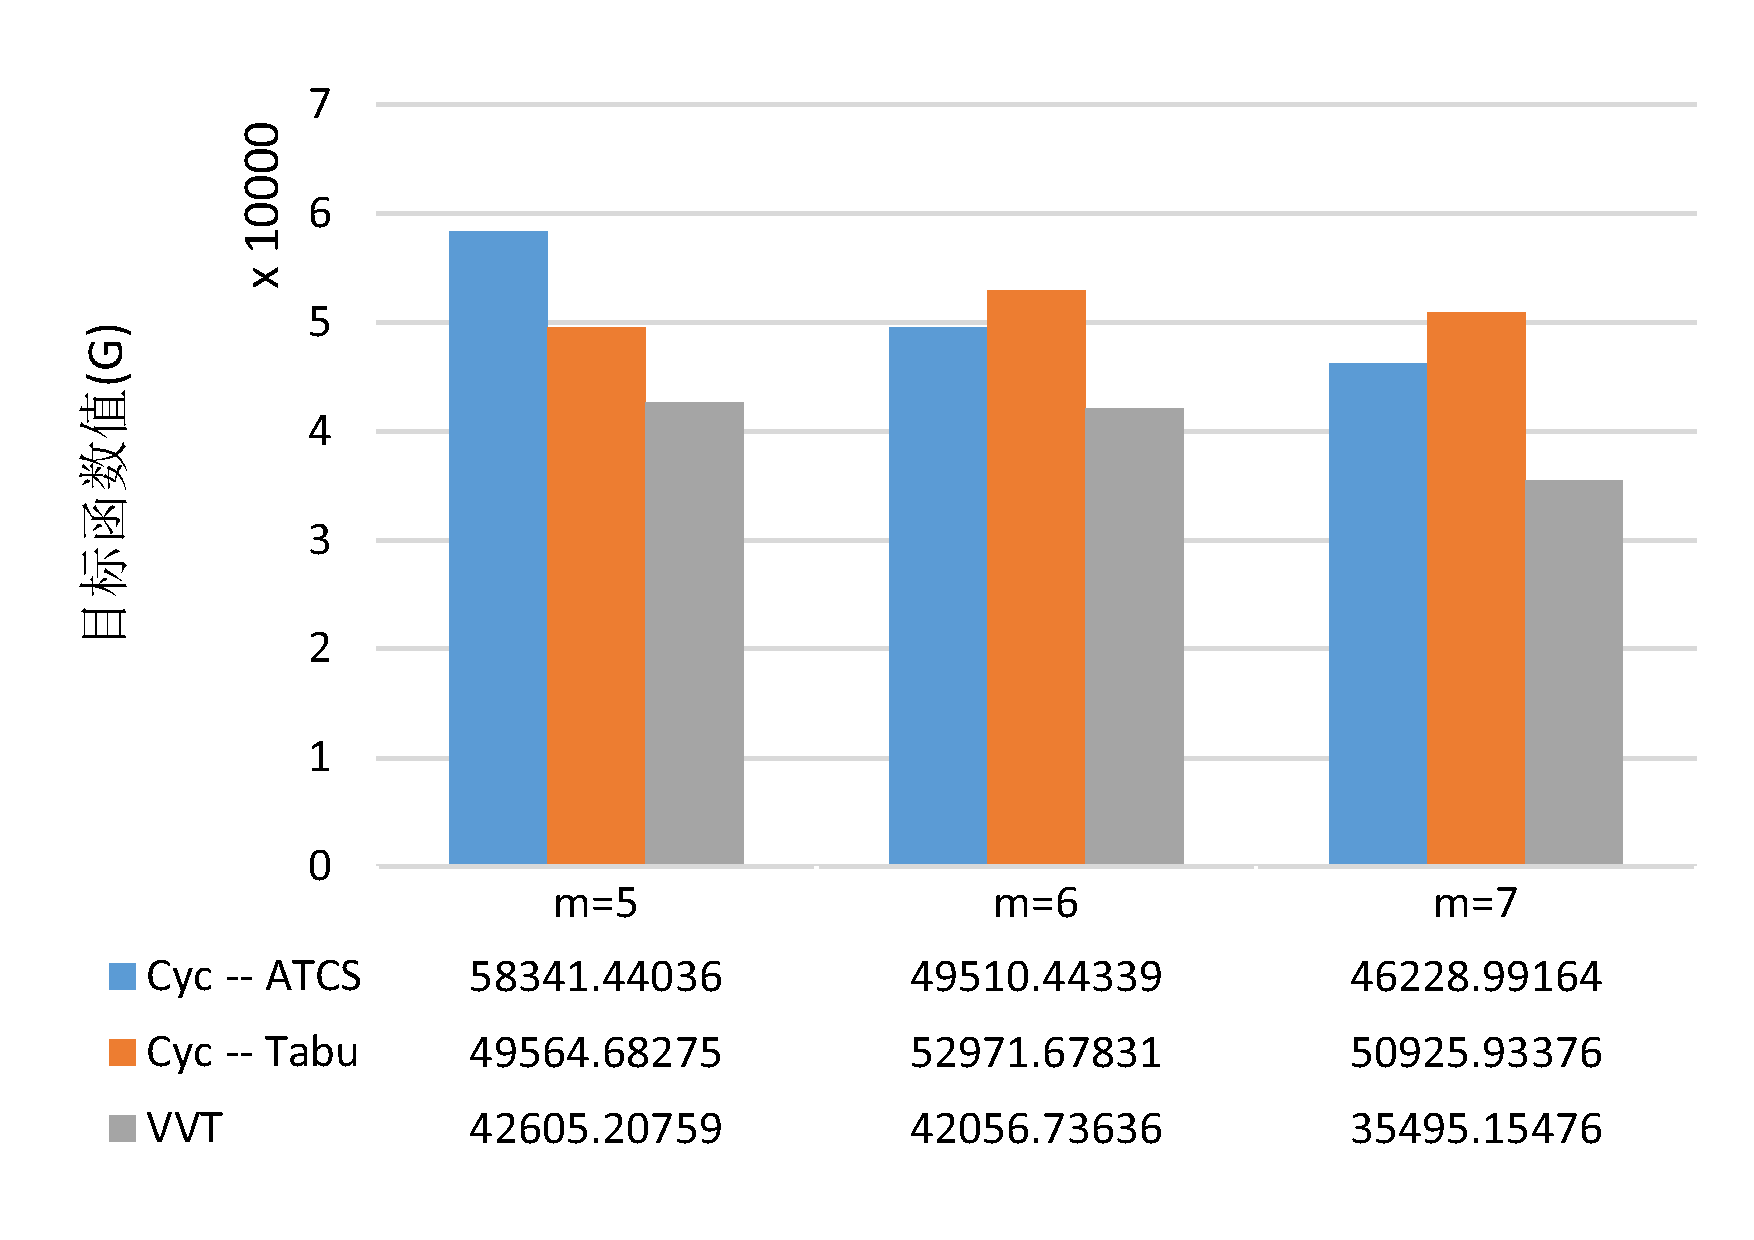
\includegraphics[height = 6cm, angle = -90]{continue_04_70}}\\
\subfloat[$n = 100$]{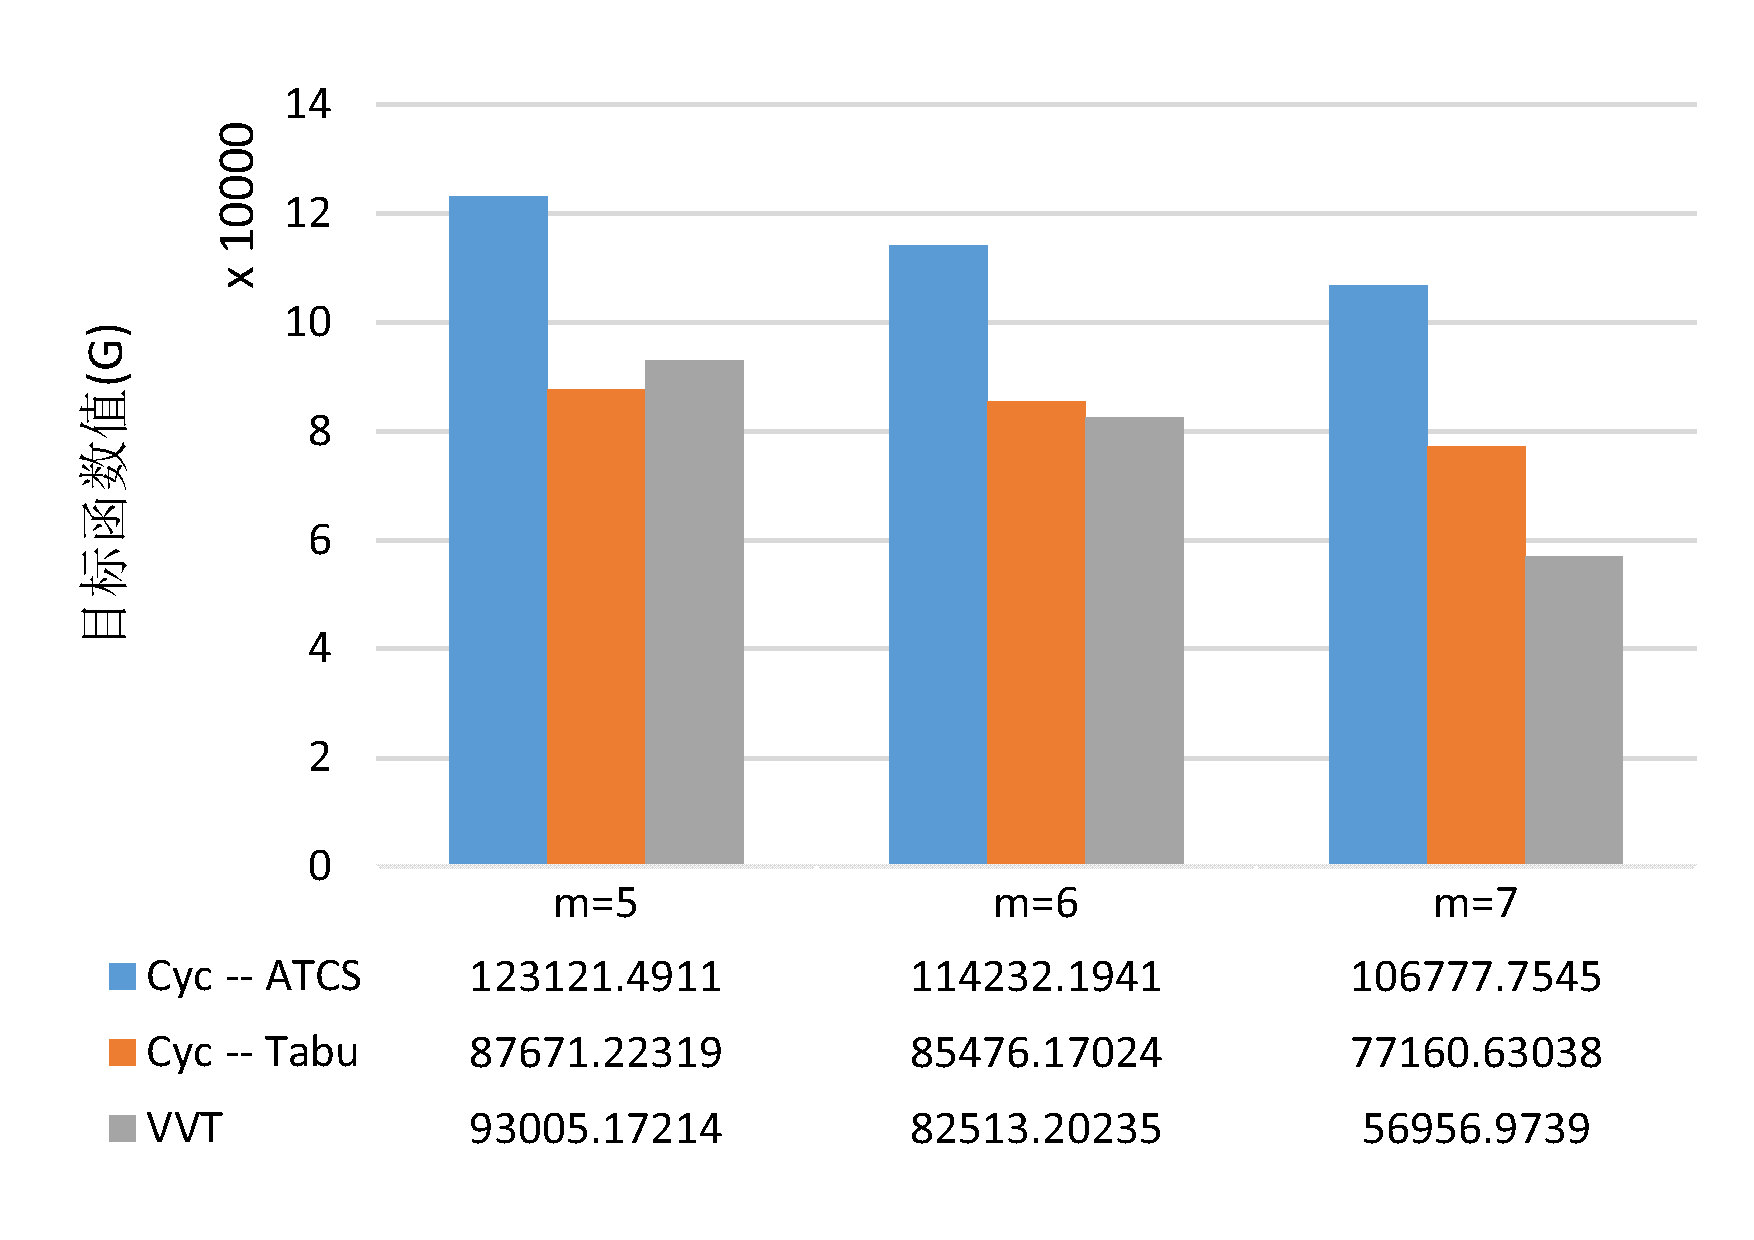
\includegraphics[height = 6cm, angle = -90]{continue_04_100}}
\subfloat[$n = 150$]{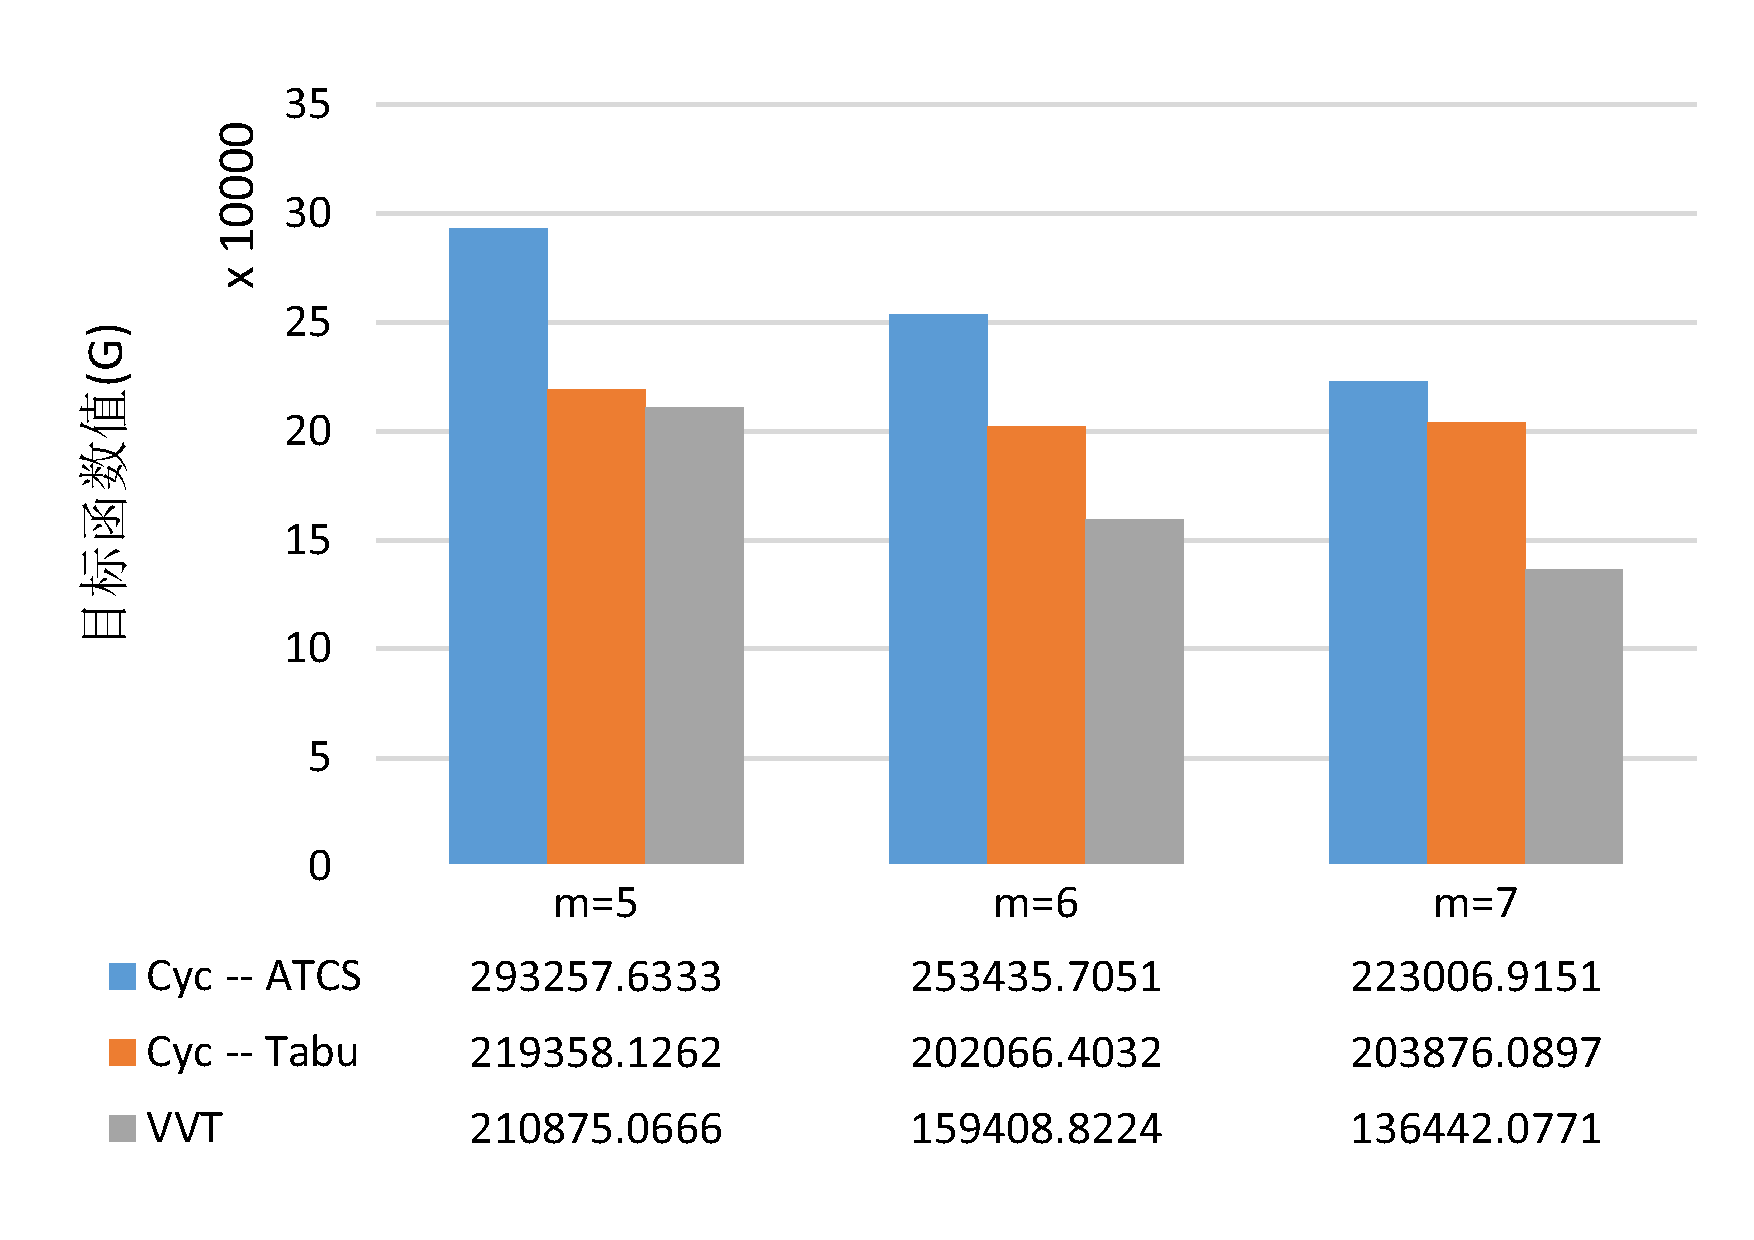
\includegraphics[height = 6cm, angle = -90]{continue_04_150}}
\subfloat[$n = 200$]{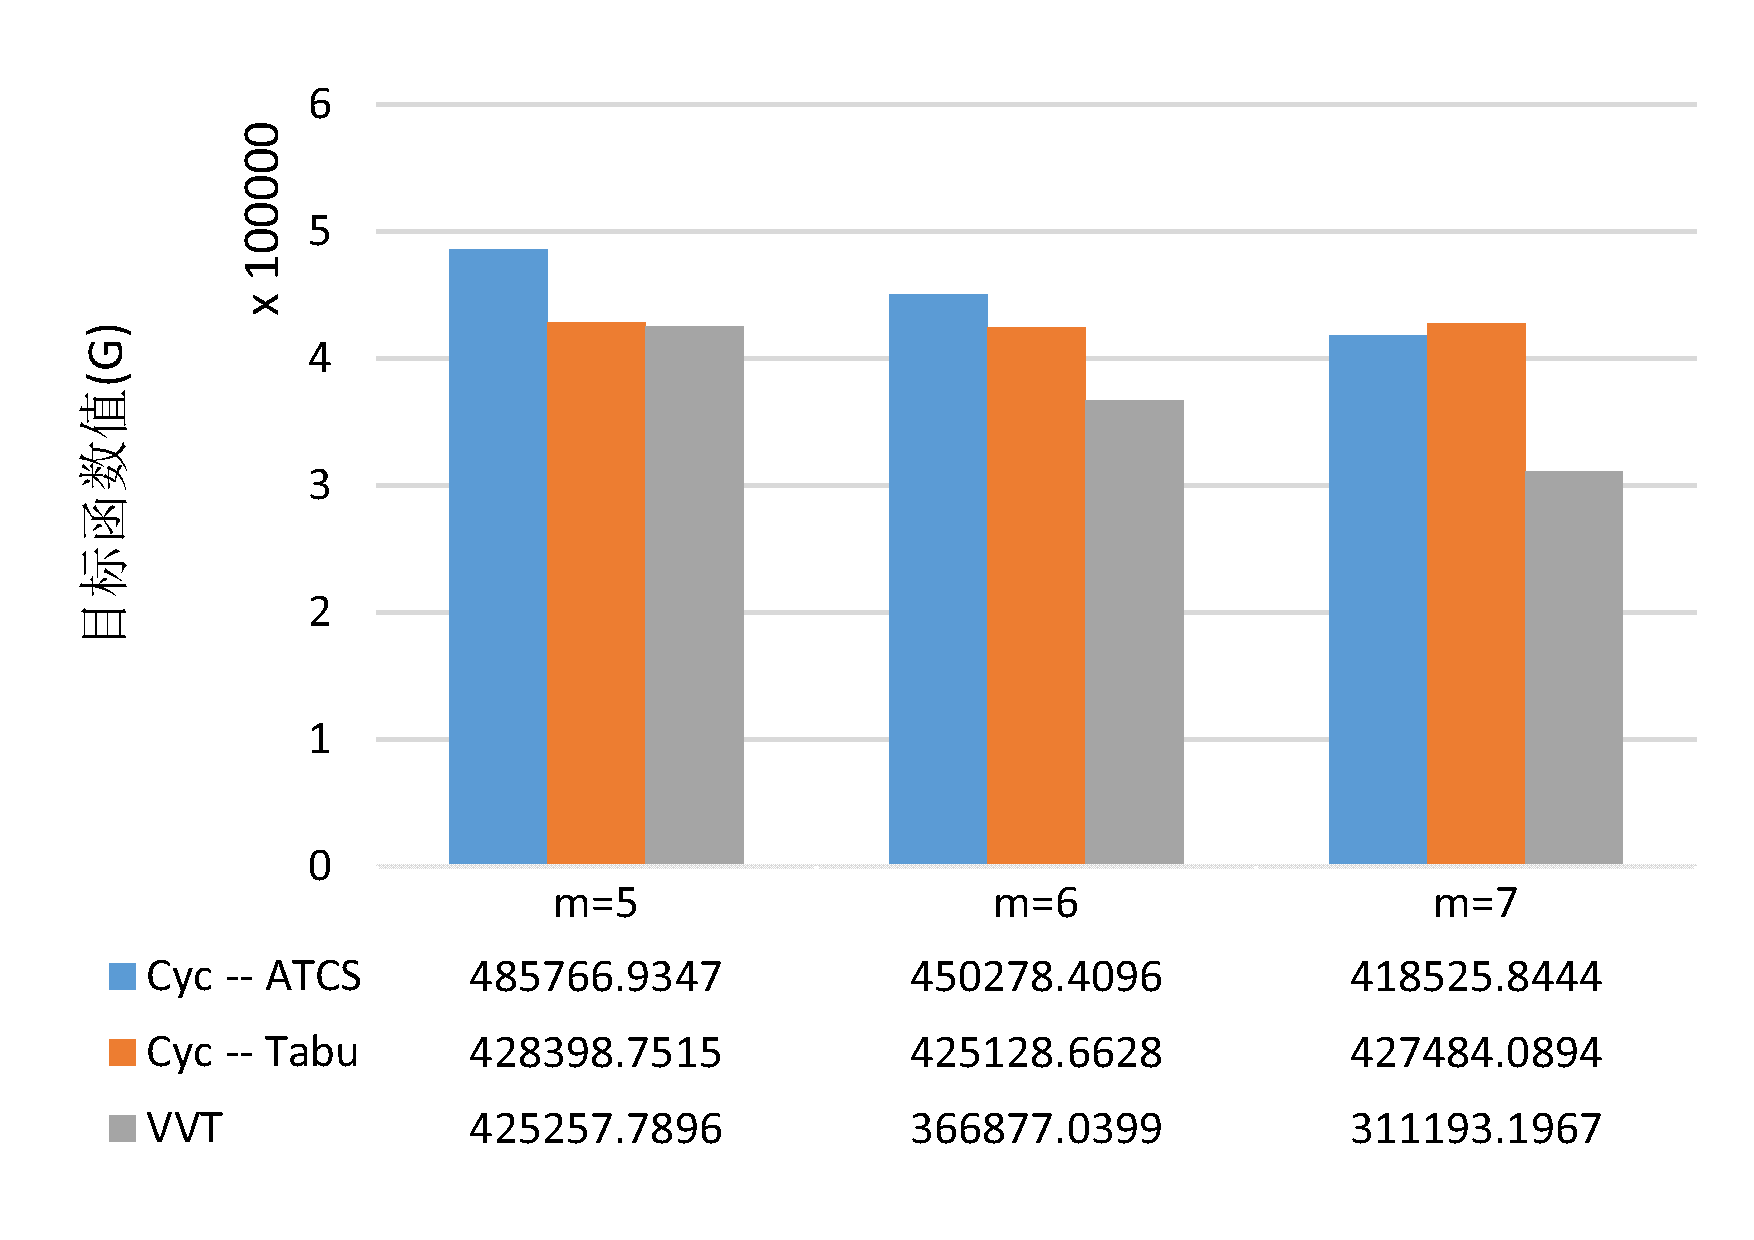
\includegraphics[height = 6cm, angle = -90]{continue_04_200}}
\subfloat[$n = 300$]{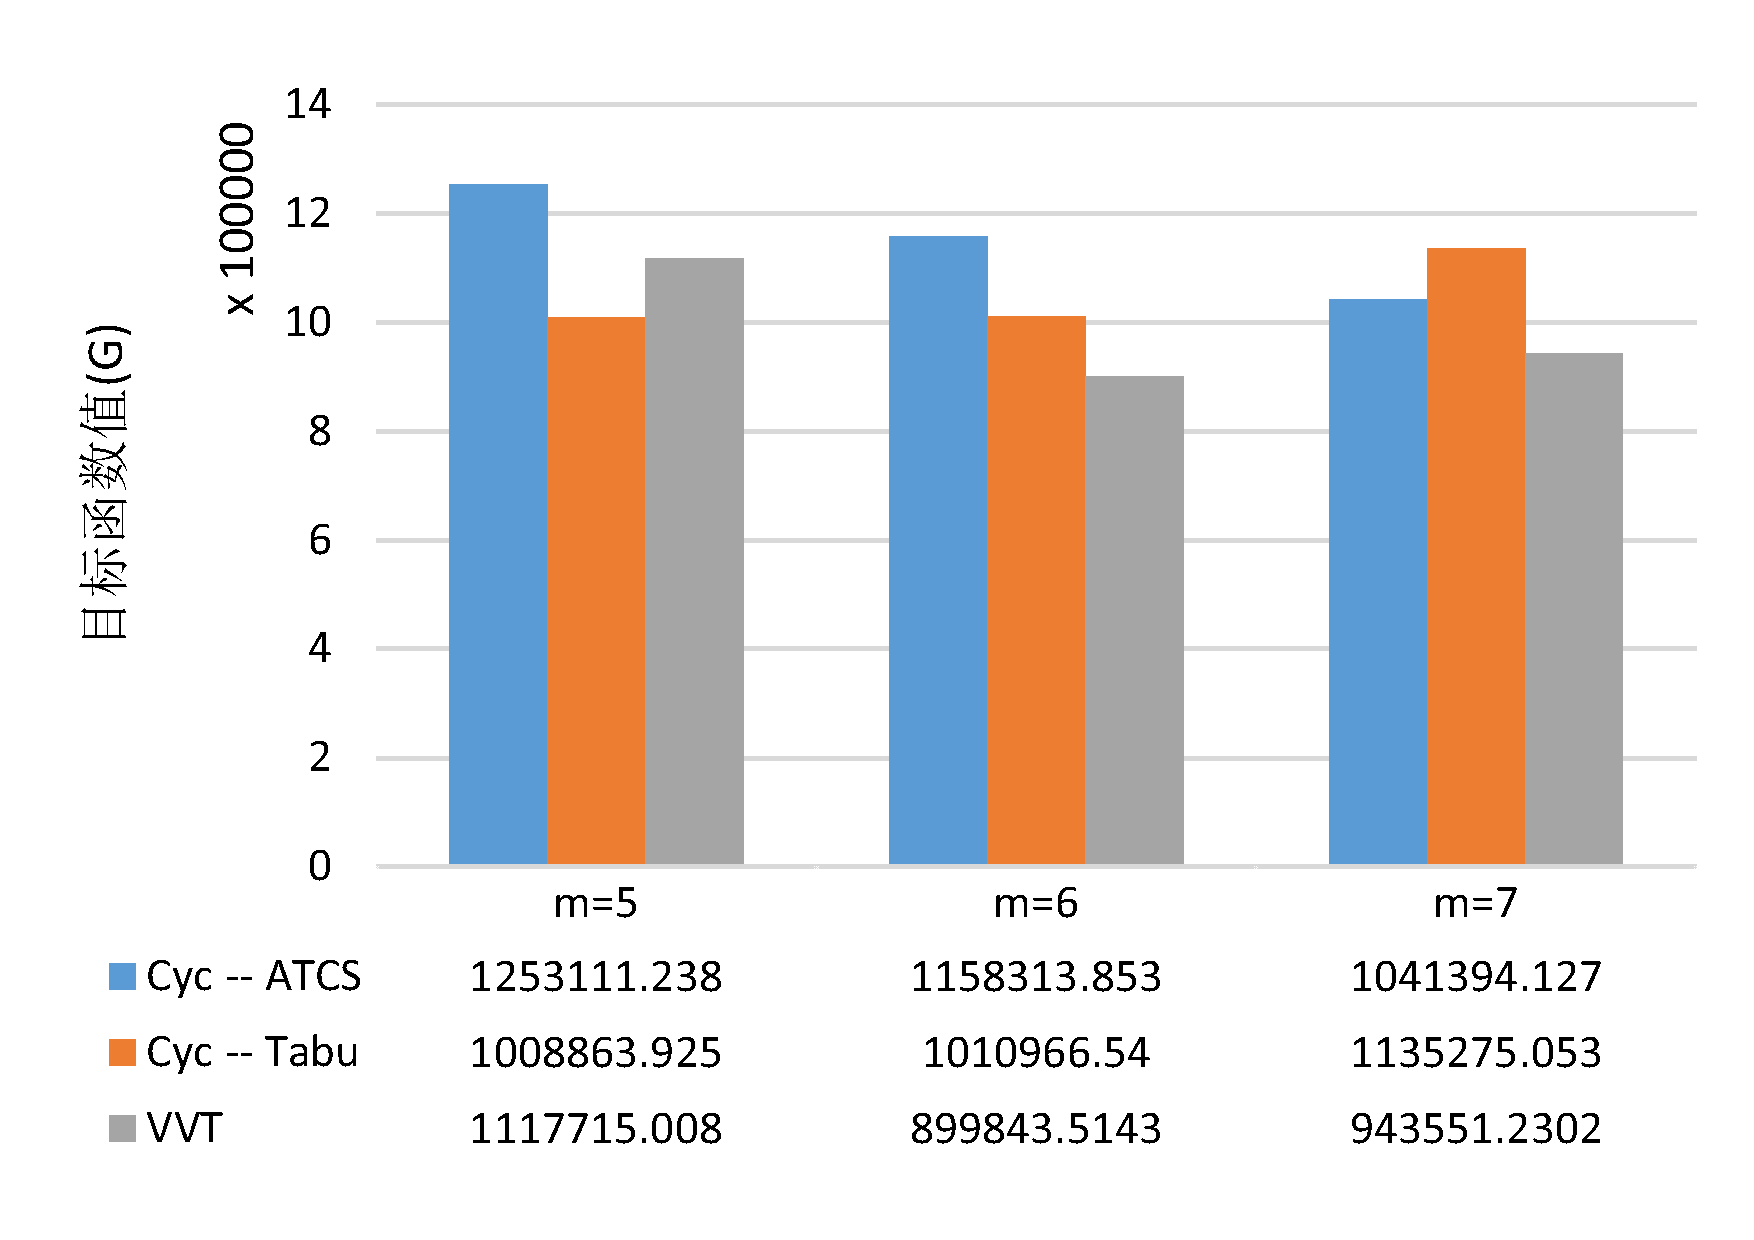
\includegraphics[height = 6cm, angle = -90]{continue_04_300}}\\
\subfloat[$n = 500$]{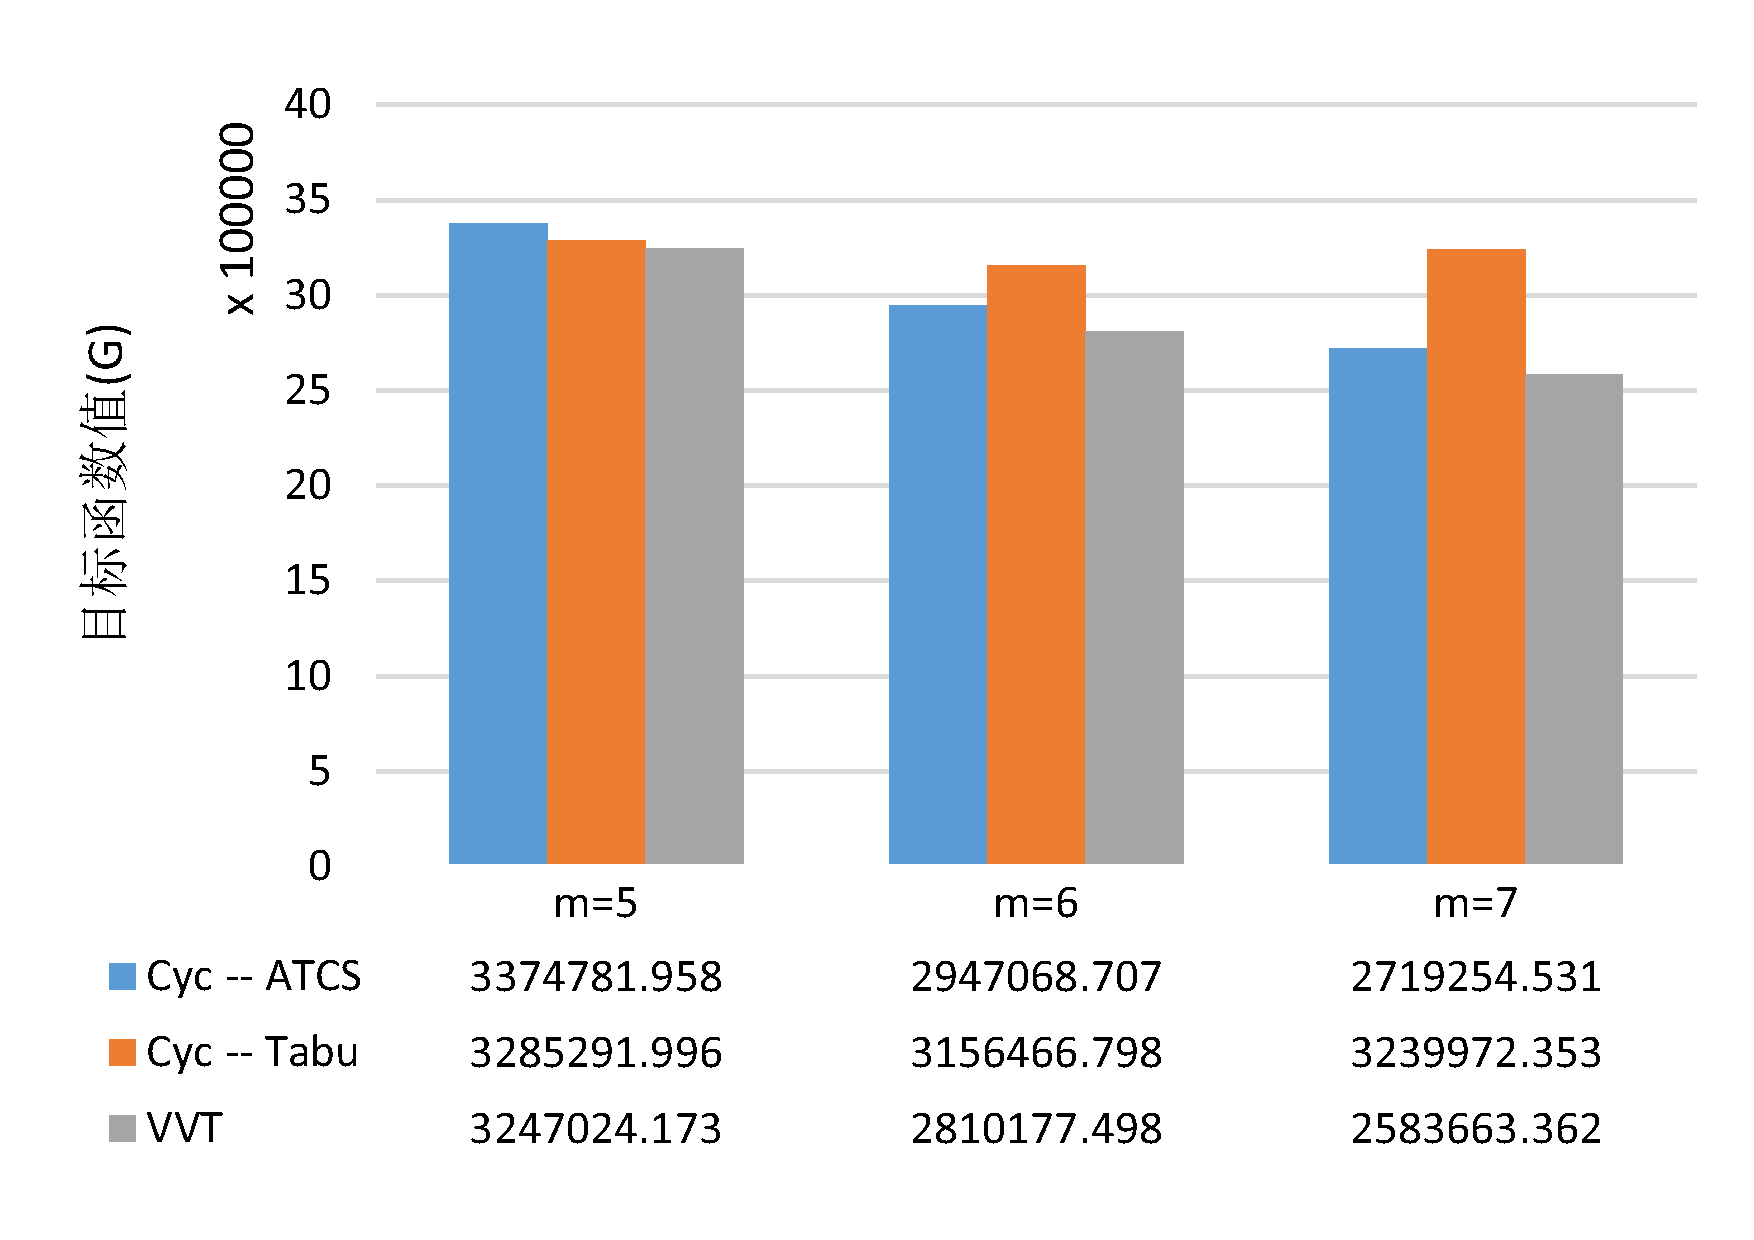
\includegraphics[height = 6cm, angle = -90]{continue_04_500}}
\subfloat[$n = 750$]{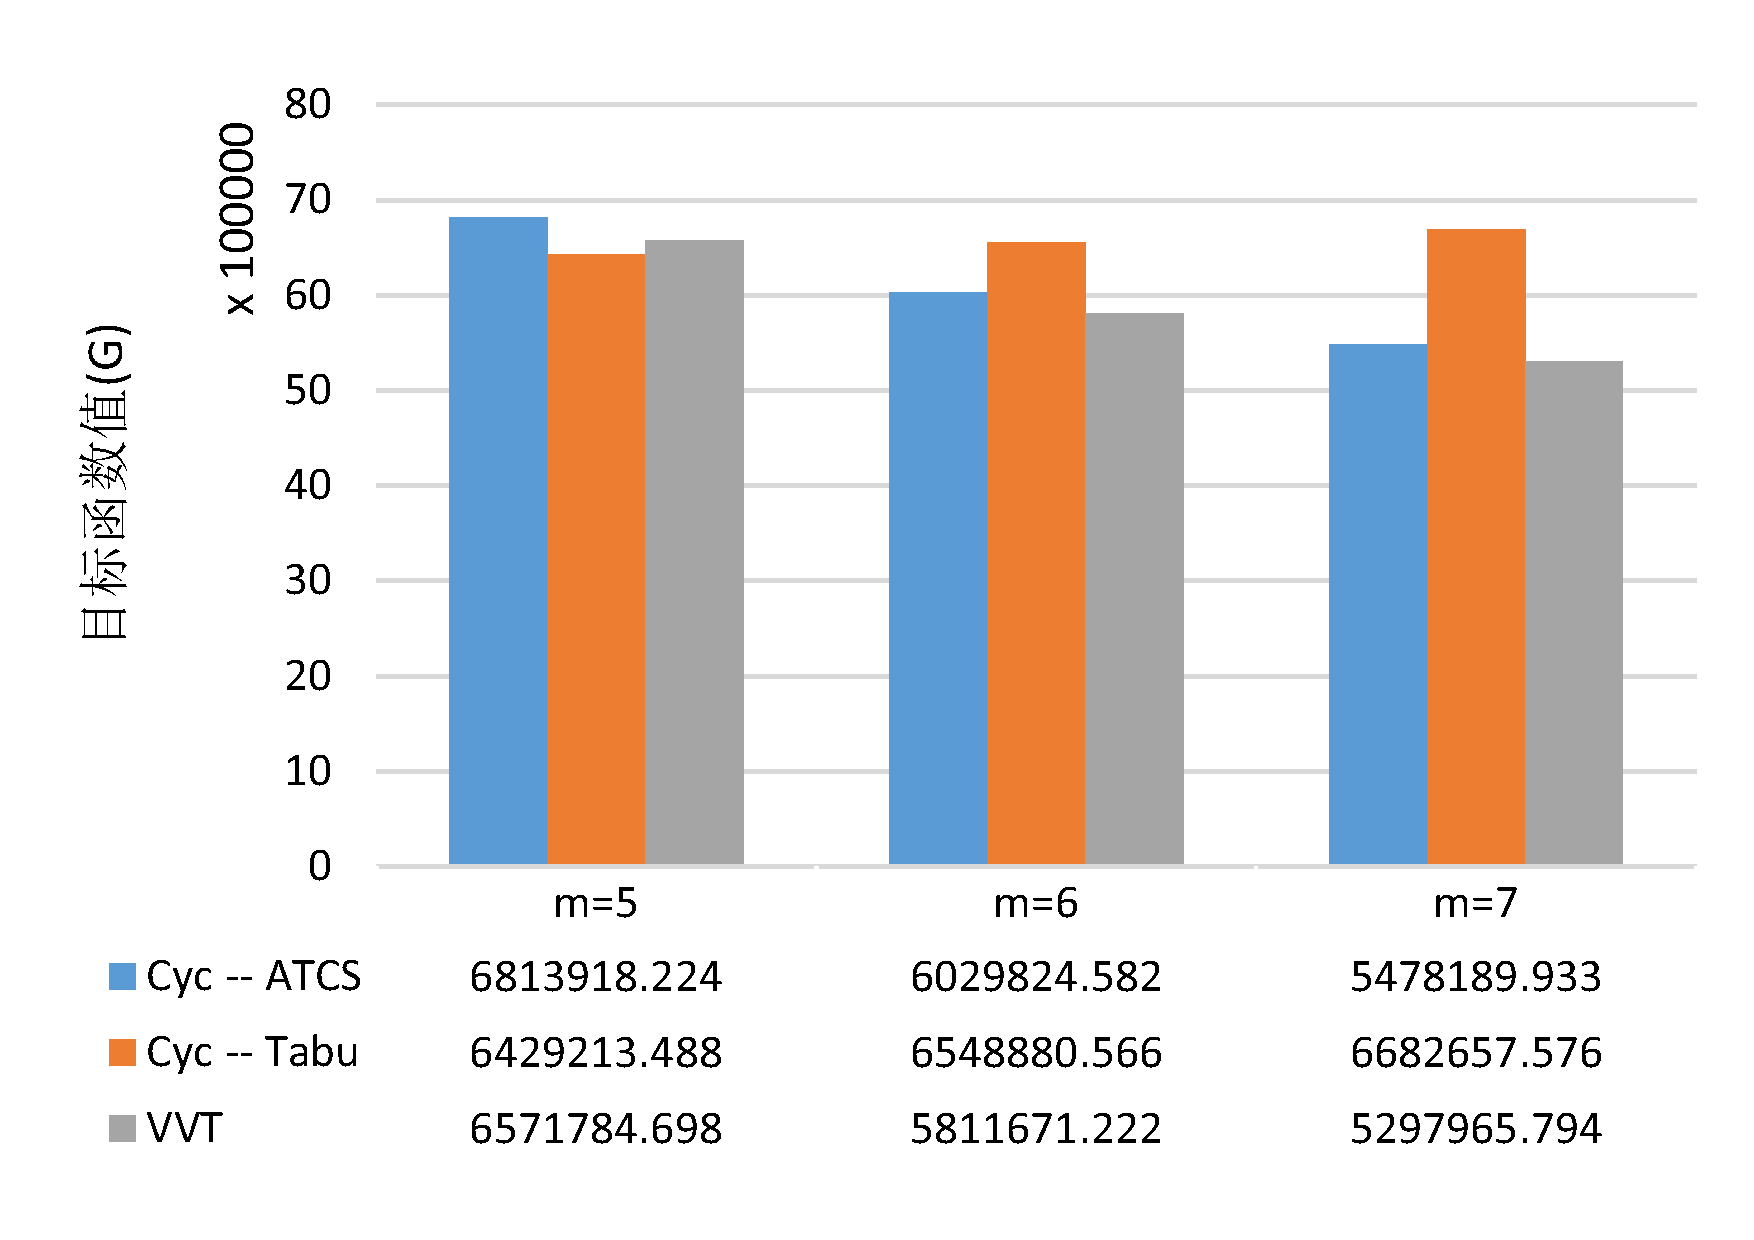
\includegraphics[height = 6cm, angle = -90]{continue_04_750}}
\subfloat[$n = 1000$]{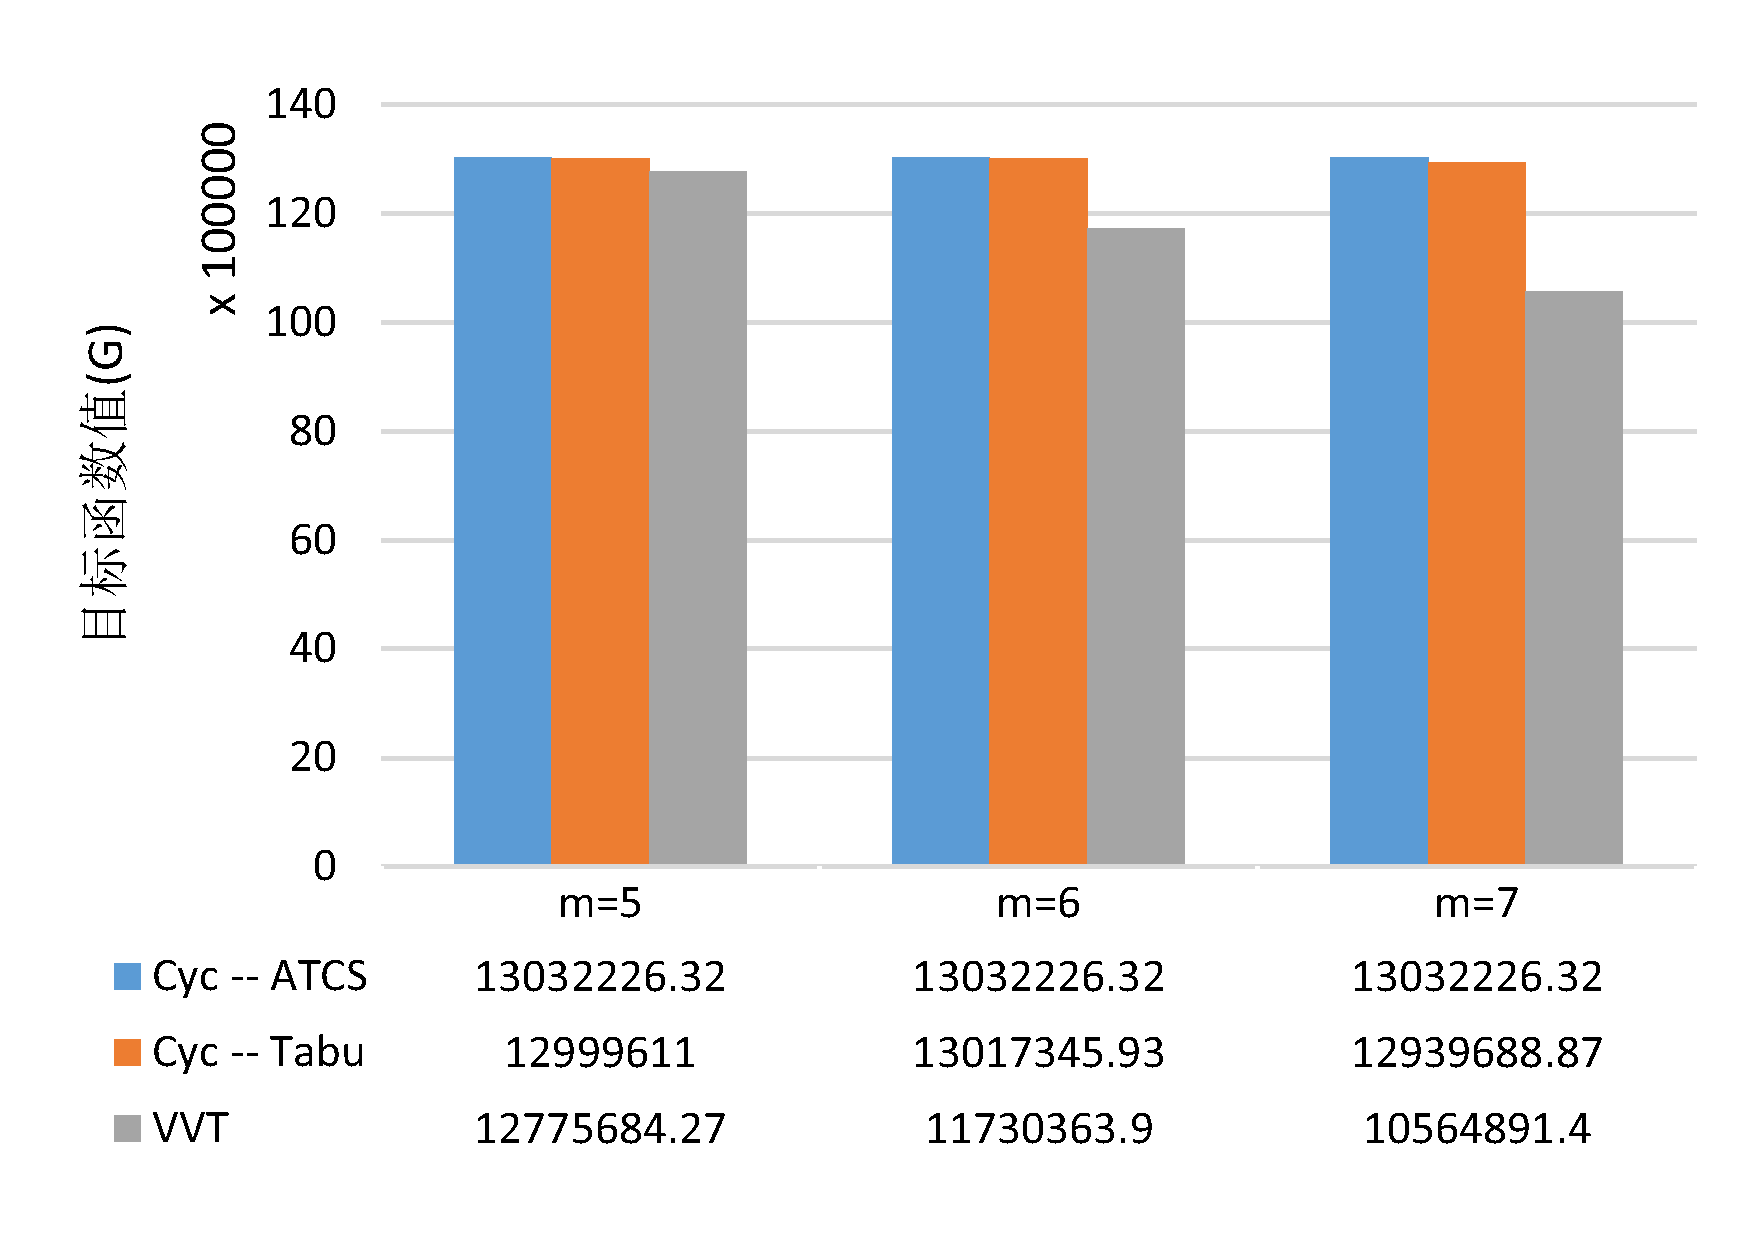
\includegraphics[height = 6cm, angle = -90]{continue_04_1000}}
\caption{\label{fig:result4}模型$2$的Cyc -- ATCS、Cyc -- Tabu、VVT 算法求解目标函数值比较$(\lambda_1 = 0.4)$}
\end{sidewaysfigure}

\begin{sidewaysfigure}
\centering
\subfloat[$n = 20$]{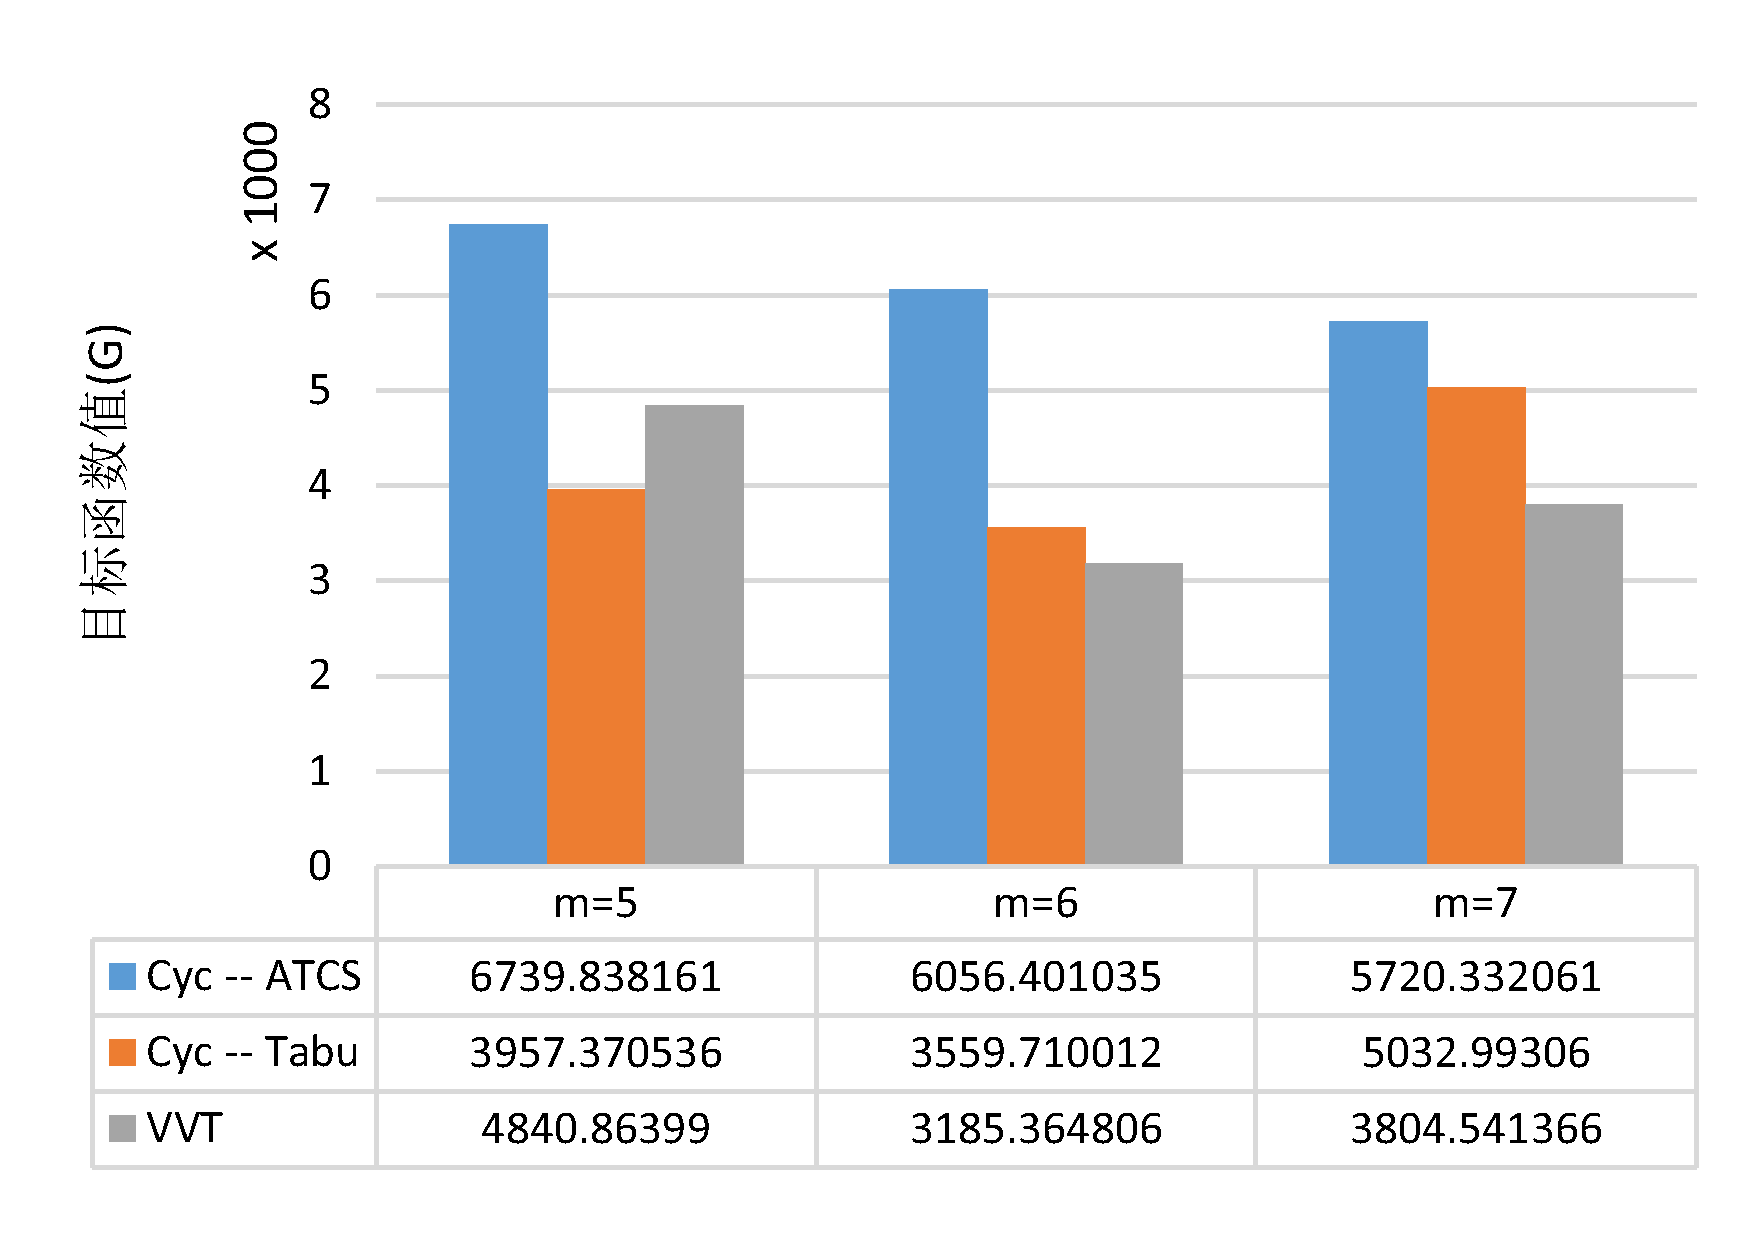
\includegraphics[height = 6cm, angle = -90]{continue_05_20}}
\subfloat[$n = 30$]{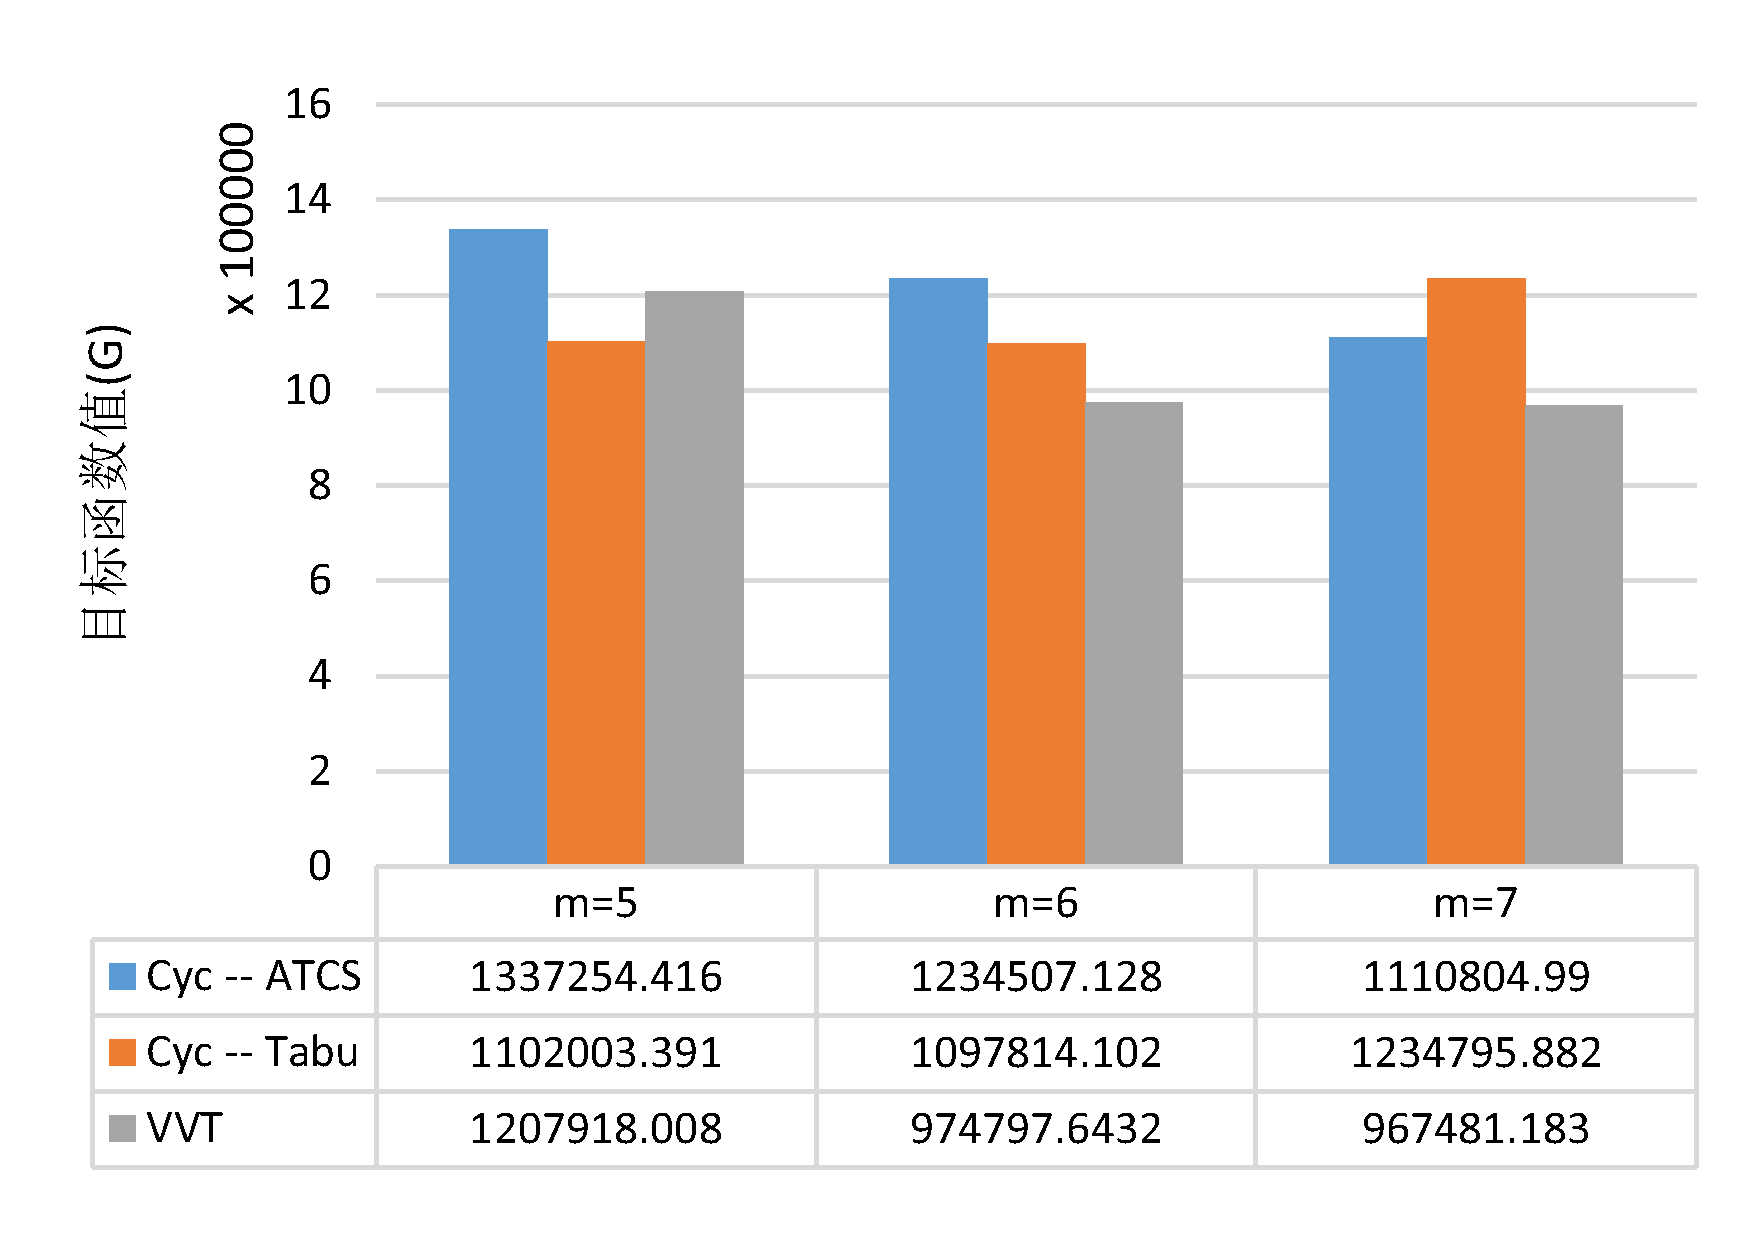
\includegraphics[height = 6cm, angle = -90]{continue_05_300}}
\subfloat[$n = 50$]{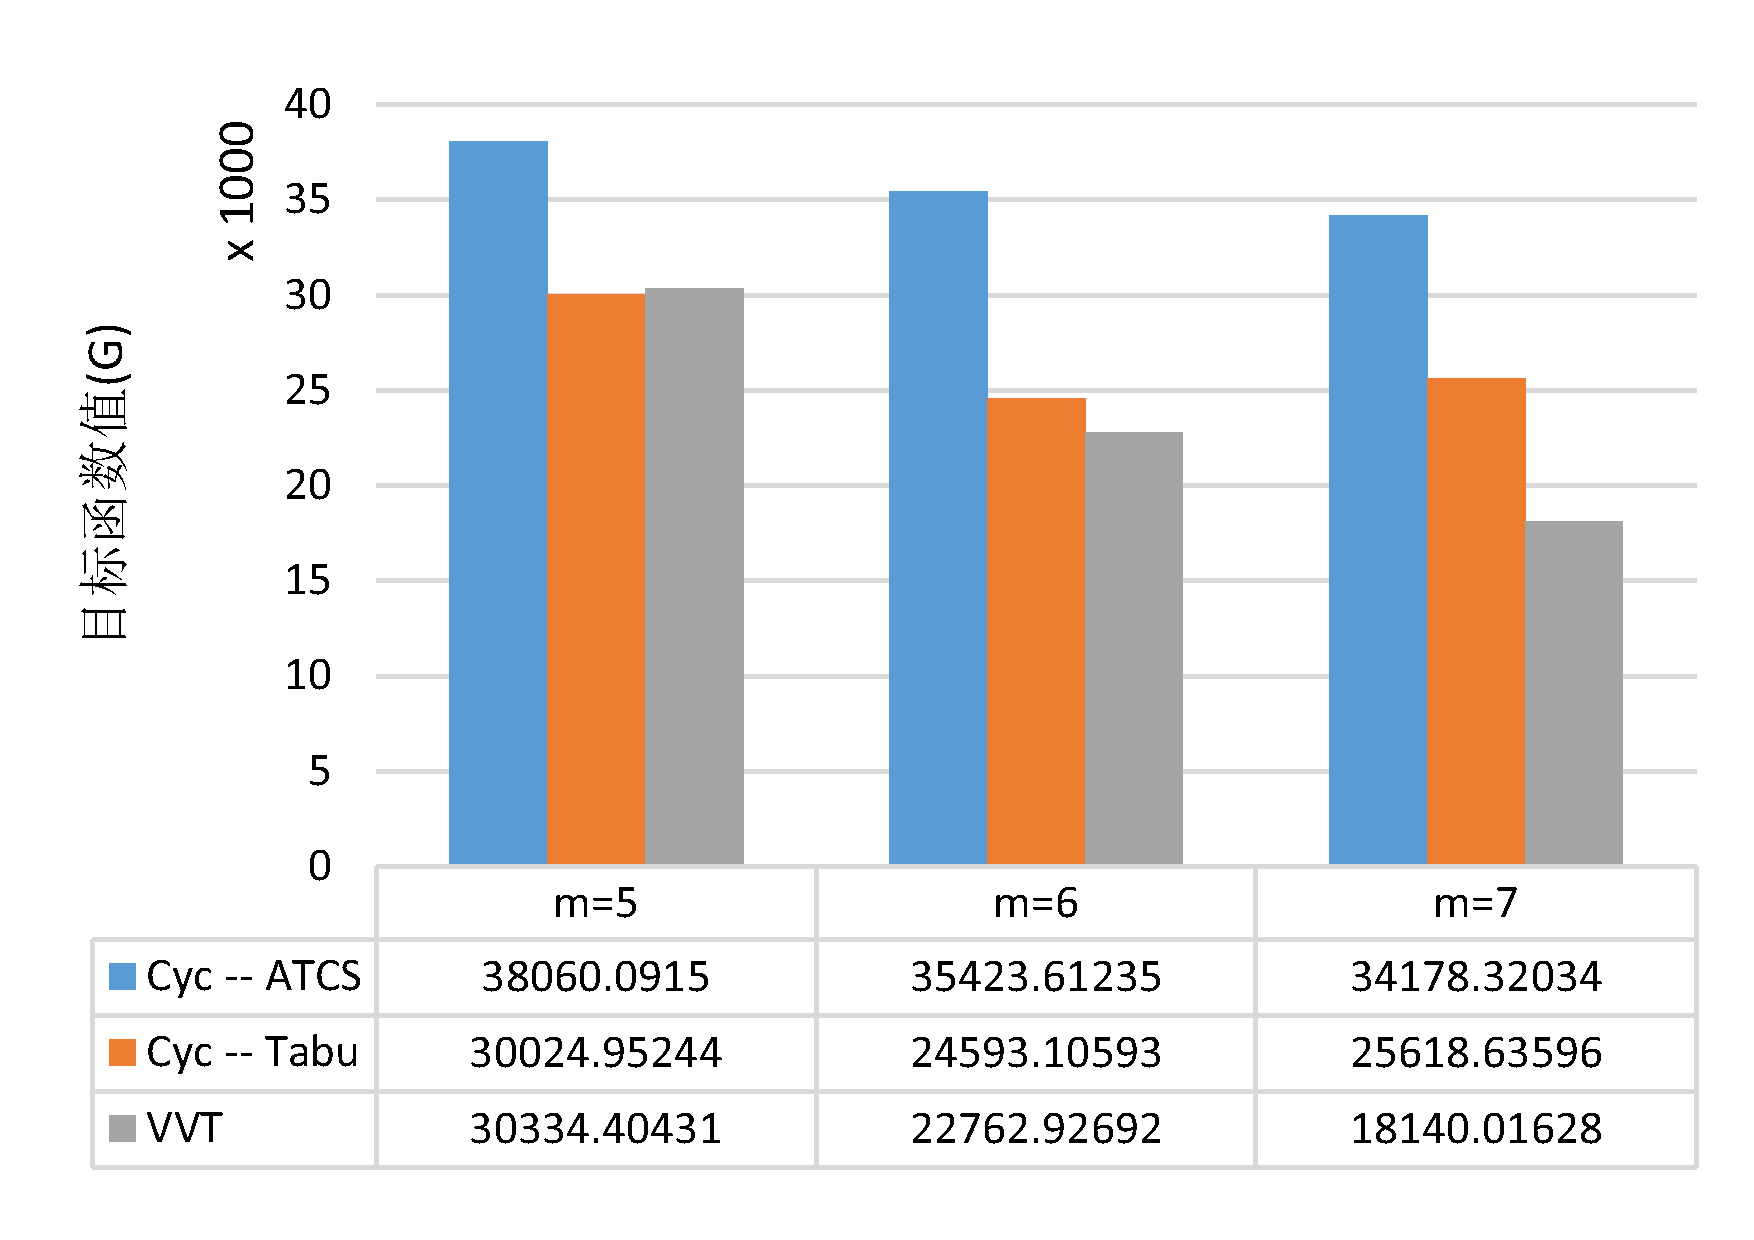
\includegraphics[height = 6cm, angle = -90]{continue_05_50}}
\subfloat[$n = 70$]{\includegraphics[height = 6cm, angle = -90]{continue_05_70}}\\
\subfloat[$n = 100$]{\includegraphics[height = 6cm, angle = -90]{continue_05_100}}
\subfloat[$n = 150$]{\includegraphics[height = 6cm, angle = -90]{continue_05_150}}
\subfloat[$n = 200$]{\includegraphics[height = 6cm, angle = -90]{continue_05_200}}
\subfloat[$n = 300$]{\includegraphics[height = 6cm, angle = -90]{continue_05_300}}\\
\subfloat[$n = 500$]{\includegraphics[height = 6cm, angle = -90]{continue_05_500}}
\subfloat[$n = 750$]{\includegraphics[height = 6cm, angle = -90]{continue_05_750}}
\subfloat[$n = 1000$]{\includegraphics[height = 6cm, angle = -90]{continue_05_1000}}
\caption{\label{fig:result5}模型$2$的Cyc -- ATCS、Cyc -- Tabu、VVT 算法求解目标函数值比较$(\lambda_1 = 0.5)$}
\end{sidewaysfigure}

\begin{sidewaysfigure}
\centering
\subfloat[$n = 20$]{\includegraphics[height = 6cm, angle = -90]{continue_06_20}}
\subfloat[$n = 30$]{\includegraphics[height = 6cm, angle = -90]{continue_06_300}}
\subfloat[$n = 50$]{\includegraphics[height = 6cm, angle = -90]{continue_06_50}}
\subfloat[$n = 70$]{\includegraphics[height = 6cm, angle = -90]{continue_06_70}}\\
\subfloat[$n = 100$]{\includegraphics[height = 6cm, angle = -90]{continue_06_100}}
\subfloat[$n = 150$]{\includegraphics[height = 6cm, angle = -90]{continue_06_150}}
\subfloat[$n = 200$]{\includegraphics[height = 6cm, angle = -90]{continue_06_200}}
\subfloat[$n = 300$]{\includegraphics[height = 6cm, angle = -90]{continue_06_300}}\\
\subfloat[$n = 500$]{\includegraphics[height = 6cm, angle = -90]{continue_06_500}}
\subfloat[$n = 750$]{\includegraphics[height = 6cm, angle = -90]{continue_06_750}}
\subfloat[$n = 1000$]{\includegraphics[height = 6cm, angle = -90]{continue_06_1000}}
\caption{\label{fig:result6}模型$2$的Cyc -- ATCS、Cyc -- Tabu、VVT 算法求解目标函数值比较$(\lambda_1 = 0.6)$}
\end{sidewaysfigure}

\begin{sidewaysfigure}
\centering
\subfloat[$n = 20$]{\includegraphics[height = 6cm, angle = -90]{Rb_04_20}}
\subfloat[$n = 30$]{\includegraphics[height = 6cm, angle = -90]{Rb_04_300}}
\subfloat[$n = 50$]{\includegraphics[height = 6cm, angle = -90]{Rb_04_50}}
\subfloat[$n = 70$]{\includegraphics[height = 6cm, angle = -90]{Rb_04_70}}\\
\subfloat[$n = 100$]{\includegraphics[height = 6cm, angle = -90]{Rb_04_100}}
\subfloat[$n = 150$]{\includegraphics[height = 6cm, angle = -90]{Rb_04_150}}
\subfloat[$n = 200$]{\includegraphics[height = 6cm, angle = -90]{Rb_04_200}}
\subfloat[$n = 300$]{\includegraphics[height = 6cm, angle = -90]{Rb_04_300}}\\
\subfloat[$n = 500$]{\includegraphics[height = 6cm, angle = -90]{Rb_04_500}}
\subfloat[$n = 750$]{\includegraphics[height = 6cm, angle = -90]{Rb_04_750}}
\subfloat[$n = 1000$]{\includegraphics[height = 6cm, angle = -90]{Rb_04_1000}}
\caption{\label{fig:result7}模型$2$的Cyc -- ATCS、Cyc -- Tabu、VVT 算法求解流水线均衡率比较$(\lambda_1 = 0.4)$}
\end{sidewaysfigure}

\begin{sidewaysfigure}
\centering
\subfloat[$n = 20$]{\includegraphics[height = 6cm, angle = -90]{Rb_05_20}}
\subfloat[$n = 30$]{\includegraphics[height = 6cm, angle = -90]{Rb_05_300}}
\subfloat[$n = 50$]{\includegraphics[height = 6cm, angle = -90]{Rb_05_50}}
\subfloat[$n = 70$]{\includegraphics[height = 6cm, angle = -90]{Rb_05_70}}\\
\subfloat[$n = 100$]{\includegraphics[height = 6cm, angle = -90]{Rb_05_100}}
\subfloat[$n = 150$]{\includegraphics[height = 6cm, angle = -90]{Rb_05_150}}
\subfloat[$n = 200$]{\includegraphics[height = 6cm, angle = -90]{Rb_05_200}}
\subfloat[$n = 300$]{\includegraphics[height = 6cm, angle = -90]{Rb_05_300}}\\
\subfloat[$n = 500$]{\includegraphics[height = 6cm, angle = -90]{Rb_05_500}}
\subfloat[$n = 750$]{\includegraphics[height = 6cm, angle = -90]{Rb_05_750}}
\subfloat[$n = 1000$]{\includegraphics[height = 6cm, angle = -90]{Rb_05_1000}}
\caption{\label{fig:result8}模型$2$的Cyc -- ATCS、Cyc -- Tabu、VVT 算法求解流水线均衡率比较$(\lambda_1 = 0.5)$}
\end{sidewaysfigure}

\begin{sidewaysfigure}
\centering
\subfloat[$n = 20$]{\includegraphics[height = 6cm, angle = -90]{Rb_06_20}}
\subfloat[$n = 30$]{\includegraphics[height = 6cm, angle = -90]{Rb_06_300}}
\subfloat[$n = 50$]{\includegraphics[height = 6cm, angle = -90]{Rb_06_50}}
\subfloat[$n = 70$]{\includegraphics[height = 6cm, angle = -90]{Rb_06_70}}\\
\subfloat[$n = 100$]{\includegraphics[height = 6cm, angle = -90]{Rb_06_100}}
\subfloat[$n = 150$]{\includegraphics[height = 6cm, angle = -90]{Rb_06_150}}
\subfloat[$n = 200$]{\includegraphics[height = 6cm, angle = -90]{Rb_06_200}}
\subfloat[$n = 300$]{\includegraphics[height = 6cm, angle = -90]{Rb_06_300}}\\
\subfloat[$n = 500$]{\includegraphics[height = 6cm, angle = -90]{Rb_06_500}}
\subfloat[$n = 750$]{\includegraphics[height = 6cm, angle = -90]{Rb_06_750}}
\subfloat[$n = 1000$]{\includegraphics[height = 6cm, angle = -90]{Rb_06_1000}}
\caption{\label{fig:result9}模型$2$的Cyc -- ATCS、Cyc -- Tabu、VVT 算法求解流水线均衡率比较$(\lambda_1 = 0.6)$}
\end{sidewaysfigure}
\chapter{算法代码}
\begin{asparaenum}
\item experiment\_data.py
\end{asparaenum}
\lstset{	basicstyle = \tiny\ttfamily,
	keywordstyle = \color{blue}\bfseries,
	stringstyle = \color{red},
	emph = {solve},
	emphstyle = \color{Green}\bfseries,
	commentstyle = \color{CadetBlue}
	}
\begin{lstlisting}[language = Python]
import sys
sys.path.append(".\\functions")
import generate
from collections import namedtuple
Item = namedtuple("Item", ['process','due','wt','wc'])

def  h(lambda1,lambda2,tardiness,completion,wt,wc):			# define the contribution of one item for the obj function
	value = lambda1*wt*tardiness + lambda2*wc*completion
	return value

def solve(input_data):
	Data = input_data.split('\n')					# load data
	n = len(Data) -1						# get the amount of items
	print n
	items = []
	for j in xrange(n):
		data = Data[j]
		parts = data.split()
		p = int(parts[0])					# get the process time
		s = int(parts[2])						# get the setup time
		d = int(parts[3])					# get the due date
		wt = int(parts[4])					# get the tardiness weights
		wc = int(parts[5])					# get the completion weights
		items.append(Item(p+s,d,wt,wc))			# combine those item data
	print 'Data loaded!'
	J = range(n)
	m = 5
	S = []
	a = []
	tl = []
	L = []
	c = [None]*n
	for l in xrange(m):
		S.append([])
		a.append(0)
		tl.append(0)
	t = 0
	f = open(".\\result\\sky",'w')
	while J:
		if 0 in a:
			l_star = a.index(0)
			p,d,wt = [],[],[]
			for j in J:				
				item = items[j]
				p.append(item.process)
				d.append(item.due)
				wt.append(item.wt)
			orderidx = generate.Idx(t,p,d,wt)
			j_star = J[orderidx.index(max(orderidx))]
			S[l_star].append(j_star)
			J.remove(j_star)
			L.append(j_star)
			tl[l_star] = t + items[j_star].process
			c[j_star] = tl[l_star]
			a[l_star] = 1
		else:
			t_star = min(tl)
			for l in xrange(m):
				if tl[l] == t_star:
					a[l] = 0
			t = t_star
	print 'initial sloution done!'
	f.write(str(S) + '\n' + str(L) + '\n' + str(c))
	f.close()


import sys
if __name__ == '__main__':
	if len(sys.argv) > 1:
		file_location = sys.argv[1].strip()
#		output = sys.argv[2].strip()
		input_data_file = open(file_location, 'r')
		input_data = ''.join(input_data_file.readlines())
		input_data_file.close()
		solve(input_data)
\end{lstlisting}
\section{456456}
\addcontentsline{toc}{section}{附录1 毕业设计文献综述}
\addcontentsline{toc}{section}{附录2 毕业设计开题报告}
\addcontentsline{toc}{section}{附录3 毕业设计外文翻译(中文译文与外文原文)}
\hspace*{7.0mm}
\hspace*{4.0mm}
\begin{minipage}[t]{95mm}
    \songti\bfseries{
    \sectionmark{附录1 毕业设计文献综述}
    附录1 毕业设计文献综述

    \vspace*{7.0mm}

    \sectionmark{附录2 毕业设计开题报告}
    附录2 毕业设计开题报告

    \vspace*{7.0mm}

    \sectionmark{附录3 毕业设计外文翻译(中文译文与外文原文)}
    附录3 毕业设计外文翻译(中文译文与外文原文)}
\end{minipage}
            % 附录

\end{document}                                  % 结束全文
